\documentclass[11pt]{article}

    \usepackage[utf8]{inputenc}
    \usepackage[english,ukrainian]{babel}

    \usepackage[breakable]{tcolorbox}
    \usepackage{parskip} % Stop auto-indenting (to mimic markdown behaviour)
    

    % Basic figure setup, for now with no caption control since it's done
    % automatically by Pandoc (which extracts ![](path) syntax from Markdown).
    \usepackage{graphicx}
    % Maintain compatibility with old templates. Remove in nbconvert 6.0
    \let\Oldincludegraphics\includegraphics
    % Ensure that by default, figures have no caption (until we provide a
    % proper Figure object with a Caption API and a way to capture that
    % in the conversion process - todo).
    \usepackage{caption}
    \DeclareCaptionFormat{nocaption}{}
    \captionsetup{format=nocaption,aboveskip=0pt,belowskip=0pt}

    \usepackage{float}
    \floatplacement{figure}{H} % forces figures to be placed at the correct location
    \usepackage{xcolor} % Allow colors to be defined
    \usepackage{enumerate} % Needed for markdown enumerations to work
    \usepackage{geometry} % Used to adjust the document margins
    \usepackage{amsmath} % Equations
    \usepackage{amssymb} % Equations
    \usepackage{textcomp} % defines textquotesingle
    % Hack from http://tex.stackexchange.com/a/47451/13684:
    \AtBeginDocument{%
        \def\PYZsq{\textquotesingle}% Upright quotes in Pygmentized code
    }
    \usepackage{upquote} % Upright quotes for verbatim code
    \usepackage{eurosym} % defines \euro

    \usepackage{iftex}
    \ifPDFTeX
        \usepackage[T1]{fontenc}
        \IfFileExists{alphabeta.sty}{
              \usepackage{alphabeta}
          }{
              \usepackage[mathletters]{ucs}
              \usepackage[utf8x]{inputenc}
          }
    \else
        \usepackage{fontspec}
        \usepackage{unicode-math}
    \fi

    \usepackage{fancyvrb} % verbatim replacement that allows latex
    \usepackage{grffile} % extends the file name processing of package graphics
                         % to support a larger range
    \makeatletter % fix for old versions of grffile with XeLaTeX
    \@ifpackagelater{grffile}{2019/11/01}
    {
      % Do nothing on new versions
    }
    {
      \def\Gread@@xetex#1{%
        \IfFileExists{"\Gin@base".bb}%
        {\Gread@eps{\Gin@base.bb}}%
        {\Gread@@xetex@aux#1}%
      }
    }
    \makeatother
    \usepackage[Export]{adjustbox} % Used to constrain images to a maximum size
    \adjustboxset{max size={0.9\linewidth}{0.9\paperheight}}

    % The hyperref package gives us a pdf with properly built
    % internal navigation ('pdf bookmarks' for the table of contents,
    % internal cross-reference links, web links for URLs, etc.)
    \usepackage{hyperref}
    % The default LaTeX title has an obnoxious amount of whitespace. By default,
    % titling removes some of it. It also provides customization options.
    \usepackage{titling}
    \usepackage{longtable} % longtable support required by pandoc >1.10
    \usepackage{booktabs}  % table support for pandoc > 1.12.2
    \usepackage{array}     % table support for pandoc >= 2.11.3
    \usepackage{calc}      % table minipage width calculation for pandoc >= 2.11.1
    \usepackage[inline]{enumitem} % IRkernel/repr support (it uses the enumerate* environment)
    \usepackage[normalem]{ulem} % ulem is needed to support strikethroughs (\sout)
                                % normalem makes italics be italics, not underlines
    \usepackage{soul}      % strikethrough (\st) support for pandoc >= 3.0.0
    \usepackage{mathrsfs}
    

    
    % Colors for the hyperref package
    \definecolor{urlcolor}{rgb}{0,.145,.698}
    \definecolor{linkcolor}{rgb}{.71,0.21,0.01}
    \definecolor{citecolor}{rgb}{.12,.54,.11}

    % ANSI colors
    \definecolor{ansi-black}{HTML}{3E424D}
    \definecolor{ansi-black-intense}{HTML}{282C36}
    \definecolor{ansi-red}{HTML}{E75C58}
    \definecolor{ansi-red-intense}{HTML}{B22B31}
    \definecolor{ansi-green}{HTML}{00A250}
    \definecolor{ansi-green-intense}{HTML}{007427}
    \definecolor{ansi-yellow}{HTML}{DDB62B}
    \definecolor{ansi-yellow-intense}{HTML}{B27D12}
    \definecolor{ansi-blue}{HTML}{208FFB}
    \definecolor{ansi-blue-intense}{HTML}{0065CA}
    \definecolor{ansi-magenta}{HTML}{D160C4}
    \definecolor{ansi-magenta-intense}{HTML}{A03196}
    \definecolor{ansi-cyan}{HTML}{60C6C8}
    \definecolor{ansi-cyan-intense}{HTML}{258F8F}
    \definecolor{ansi-white}{HTML}{C5C1B4}
    \definecolor{ansi-white-intense}{HTML}{A1A6B2}
    \definecolor{ansi-default-inverse-fg}{HTML}{FFFFFF}
    \definecolor{ansi-default-inverse-bg}{HTML}{000000}

    % common color for the border for error outputs.
    \definecolor{outerrorbackground}{HTML}{FFDFDF}

    % commands and environments needed by pandoc snippets
    % extracted from the output of `pandoc -s`
    \providecommand{\tightlist}{%
      \setlength{\itemsep}{0pt}\setlength{\parskip}{0pt}}
    \DefineVerbatimEnvironment{Highlighting}{Verbatim}{commandchars=\\\{\}}
    % Add ',fontsize=\small' for more characters per line
    \newenvironment{Shaded}{}{}
    \newcommand{\KeywordTok}[1]{\textcolor[rgb]{0.00,0.44,0.13}{\textbf{{#1}}}}
    \newcommand{\DataTypeTok}[1]{\textcolor[rgb]{0.56,0.13,0.00}{{#1}}}
    \newcommand{\DecValTok}[1]{\textcolor[rgb]{0.25,0.63,0.44}{{#1}}}
    \newcommand{\BaseNTok}[1]{\textcolor[rgb]{0.25,0.63,0.44}{{#1}}}
    \newcommand{\FloatTok}[1]{\textcolor[rgb]{0.25,0.63,0.44}{{#1}}}
    \newcommand{\CharTok}[1]{\textcolor[rgb]{0.25,0.44,0.63}{{#1}}}
    \newcommand{\StringTok}[1]{\textcolor[rgb]{0.25,0.44,0.63}{{#1}}}
    \newcommand{\CommentTok}[1]{\textcolor[rgb]{0.38,0.63,0.69}{\textit{{#1}}}}
    \newcommand{\OtherTok}[1]{\textcolor[rgb]{0.00,0.44,0.13}{{#1}}}
    \newcommand{\AlertTok}[1]{\textcolor[rgb]{1.00,0.00,0.00}{\textbf{{#1}}}}
    \newcommand{\FunctionTok}[1]{\textcolor[rgb]{0.02,0.16,0.49}{{#1}}}
    \newcommand{\RegionMarkerTok}[1]{{#1}}
    \newcommand{\ErrorTok}[1]{\textcolor[rgb]{1.00,0.00,0.00}{\textbf{{#1}}}}
    \newcommand{\NormalTok}[1]{{#1}}

    % Additional commands for more recent versions of Pandoc
    \newcommand{\ConstantTok}[1]{\textcolor[rgb]{0.53,0.00,0.00}{{#1}}}
    \newcommand{\SpecialCharTok}[1]{\textcolor[rgb]{0.25,0.44,0.63}{{#1}}}
    \newcommand{\VerbatimStringTok}[1]{\textcolor[rgb]{0.25,0.44,0.63}{{#1}}}
    \newcommand{\SpecialStringTok}[1]{\textcolor[rgb]{0.73,0.40,0.53}{{#1}}}
    \newcommand{\ImportTok}[1]{{#1}}
    \newcommand{\DocumentationTok}[1]{\textcolor[rgb]{0.73,0.13,0.13}{\textit{{#1}}}}
    \newcommand{\AnnotationTok}[1]{\textcolor[rgb]{0.38,0.63,0.69}{\textbf{\textit{{#1}}}}}
    \newcommand{\CommentVarTok}[1]{\textcolor[rgb]{0.38,0.63,0.69}{\textbf{\textit{{#1}}}}}
    \newcommand{\VariableTok}[1]{\textcolor[rgb]{0.10,0.09,0.49}{{#1}}}
    \newcommand{\ControlFlowTok}[1]{\textcolor[rgb]{0.00,0.44,0.13}{\textbf{{#1}}}}
    \newcommand{\OperatorTok}[1]{\textcolor[rgb]{0.40,0.40,0.40}{{#1}}}
    \newcommand{\BuiltInTok}[1]{{#1}}
    \newcommand{\ExtensionTok}[1]{{#1}}
    \newcommand{\PreprocessorTok}[1]{\textcolor[rgb]{0.74,0.48,0.00}{{#1}}}
    \newcommand{\AttributeTok}[1]{\textcolor[rgb]{0.49,0.56,0.16}{{#1}}}
    \newcommand{\InformationTok}[1]{\textcolor[rgb]{0.38,0.63,0.69}{\textbf{\textit{{#1}}}}}
    \newcommand{\WarningTok}[1]{\textcolor[rgb]{0.38,0.63,0.69}{\textbf{\textit{{#1}}}}}


    % Define a nice break command that doesn't care if a line doesn't already
    % exist.
    \def\br{\hspace*{\fill} \\* }
    % Math Jax compatibility definitions
    \def\gt{>}
    \def\lt{<}
    \let\Oldtex\TeX
    \let\Oldlatex\LaTeX
    \renewcommand{\TeX}{\textrm{\Oldtex}}
    \renewcommand{\LaTeX}{\textrm{\Oldlatex}}
    % Document parameters
    % Document title
    \title{laguerre}
    
    
    
    
    
    
    
% Pygments definitions
\makeatletter
\def\PY@reset{\let\PY@it=\relax \let\PY@bf=\relax%
    \let\PY@ul=\relax \let\PY@tc=\relax%
    \let\PY@bc=\relax \let\PY@ff=\relax}
\def\PY@tok#1{\csname PY@tok@#1\endcsname}
\def\PY@toks#1+{\ifx\relax#1\empty\else%
    \PY@tok{#1}\expandafter\PY@toks\fi}
\def\PY@do#1{\PY@bc{\PY@tc{\PY@ul{%
    \PY@it{\PY@bf{\PY@ff{#1}}}}}}}
\def\PY#1#2{\PY@reset\PY@toks#1+\relax+\PY@do{#2}}

\@namedef{PY@tok@w}{\def\PY@tc##1{\textcolor[rgb]{0.73,0.73,0.73}{##1}}}
\@namedef{PY@tok@c}{\let\PY@it=\textit\def\PY@tc##1{\textcolor[rgb]{0.24,0.48,0.48}{##1}}}
\@namedef{PY@tok@cp}{\def\PY@tc##1{\textcolor[rgb]{0.61,0.40,0.00}{##1}}}
\@namedef{PY@tok@k}{\let\PY@bf=\textbf\def\PY@tc##1{\textcolor[rgb]{0.00,0.50,0.00}{##1}}}
\@namedef{PY@tok@kp}{\def\PY@tc##1{\textcolor[rgb]{0.00,0.50,0.00}{##1}}}
\@namedef{PY@tok@kt}{\def\PY@tc##1{\textcolor[rgb]{0.69,0.00,0.25}{##1}}}
\@namedef{PY@tok@o}{\def\PY@tc##1{\textcolor[rgb]{0.40,0.40,0.40}{##1}}}
\@namedef{PY@tok@ow}{\let\PY@bf=\textbf\def\PY@tc##1{\textcolor[rgb]{0.67,0.13,1.00}{##1}}}
\@namedef{PY@tok@nb}{\def\PY@tc##1{\textcolor[rgb]{0.00,0.50,0.00}{##1}}}
\@namedef{PY@tok@nf}{\def\PY@tc##1{\textcolor[rgb]{0.00,0.00,1.00}{##1}}}
\@namedef{PY@tok@nc}{\let\PY@bf=\textbf\def\PY@tc##1{\textcolor[rgb]{0.00,0.00,1.00}{##1}}}
\@namedef{PY@tok@nn}{\let\PY@bf=\textbf\def\PY@tc##1{\textcolor[rgb]{0.00,0.00,1.00}{##1}}}
\@namedef{PY@tok@ne}{\let\PY@bf=\textbf\def\PY@tc##1{\textcolor[rgb]{0.80,0.25,0.22}{##1}}}
\@namedef{PY@tok@nv}{\def\PY@tc##1{\textcolor[rgb]{0.10,0.09,0.49}{##1}}}
\@namedef{PY@tok@no}{\def\PY@tc##1{\textcolor[rgb]{0.53,0.00,0.00}{##1}}}
\@namedef{PY@tok@nl}{\def\PY@tc##1{\textcolor[rgb]{0.46,0.46,0.00}{##1}}}
\@namedef{PY@tok@ni}{\let\PY@bf=\textbf\def\PY@tc##1{\textcolor[rgb]{0.44,0.44,0.44}{##1}}}
\@namedef{PY@tok@na}{\def\PY@tc##1{\textcolor[rgb]{0.41,0.47,0.13}{##1}}}
\@namedef{PY@tok@nt}{\let\PY@bf=\textbf\def\PY@tc##1{\textcolor[rgb]{0.00,0.50,0.00}{##1}}}
\@namedef{PY@tok@nd}{\def\PY@tc##1{\textcolor[rgb]{0.67,0.13,1.00}{##1}}}
\@namedef{PY@tok@s}{\def\PY@tc##1{\textcolor[rgb]{0.73,0.13,0.13}{##1}}}
\@namedef{PY@tok@sd}{\let\PY@it=\textit\def\PY@tc##1{\textcolor[rgb]{0.73,0.13,0.13}{##1}}}
\@namedef{PY@tok@si}{\let\PY@bf=\textbf\def\PY@tc##1{\textcolor[rgb]{0.64,0.35,0.47}{##1}}}
\@namedef{PY@tok@se}{\let\PY@bf=\textbf\def\PY@tc##1{\textcolor[rgb]{0.67,0.36,0.12}{##1}}}
\@namedef{PY@tok@sr}{\def\PY@tc##1{\textcolor[rgb]{0.64,0.35,0.47}{##1}}}
\@namedef{PY@tok@ss}{\def\PY@tc##1{\textcolor[rgb]{0.10,0.09,0.49}{##1}}}
\@namedef{PY@tok@sx}{\def\PY@tc##1{\textcolor[rgb]{0.00,0.50,0.00}{##1}}}
\@namedef{PY@tok@m}{\def\PY@tc##1{\textcolor[rgb]{0.40,0.40,0.40}{##1}}}
\@namedef{PY@tok@gh}{\let\PY@bf=\textbf\def\PY@tc##1{\textcolor[rgb]{0.00,0.00,0.50}{##1}}}
\@namedef{PY@tok@gu}{\let\PY@bf=\textbf\def\PY@tc##1{\textcolor[rgb]{0.50,0.00,0.50}{##1}}}
\@namedef{PY@tok@gd}{\def\PY@tc##1{\textcolor[rgb]{0.63,0.00,0.00}{##1}}}
\@namedef{PY@tok@gi}{\def\PY@tc##1{\textcolor[rgb]{0.00,0.52,0.00}{##1}}}
\@namedef{PY@tok@gr}{\def\PY@tc##1{\textcolor[rgb]{0.89,0.00,0.00}{##1}}}
\@namedef{PY@tok@ge}{\let\PY@it=\textit}
\@namedef{PY@tok@gs}{\let\PY@bf=\textbf}
\@namedef{PY@tok@ges}{\let\PY@bf=\textbf\let\PY@it=\textit}
\@namedef{PY@tok@gp}{\let\PY@bf=\textbf\def\PY@tc##1{\textcolor[rgb]{0.00,0.00,0.50}{##1}}}
\@namedef{PY@tok@go}{\def\PY@tc##1{\textcolor[rgb]{0.44,0.44,0.44}{##1}}}
\@namedef{PY@tok@gt}{\def\PY@tc##1{\textcolor[rgb]{0.00,0.27,0.87}{##1}}}
\@namedef{PY@tok@err}{\def\PY@bc##1{{\setlength{\fboxsep}{\string -\fboxrule}\fcolorbox[rgb]{1.00,0.00,0.00}{1,1,1}{\strut ##1}}}}
\@namedef{PY@tok@kc}{\let\PY@bf=\textbf\def\PY@tc##1{\textcolor[rgb]{0.00,0.50,0.00}{##1}}}
\@namedef{PY@tok@kd}{\let\PY@bf=\textbf\def\PY@tc##1{\textcolor[rgb]{0.00,0.50,0.00}{##1}}}
\@namedef{PY@tok@kn}{\let\PY@bf=\textbf\def\PY@tc##1{\textcolor[rgb]{0.00,0.50,0.00}{##1}}}
\@namedef{PY@tok@kr}{\let\PY@bf=\textbf\def\PY@tc##1{\textcolor[rgb]{0.00,0.50,0.00}{##1}}}
\@namedef{PY@tok@bp}{\def\PY@tc##1{\textcolor[rgb]{0.00,0.50,0.00}{##1}}}
\@namedef{PY@tok@fm}{\def\PY@tc##1{\textcolor[rgb]{0.00,0.00,1.00}{##1}}}
\@namedef{PY@tok@vc}{\def\PY@tc##1{\textcolor[rgb]{0.10,0.09,0.49}{##1}}}
\@namedef{PY@tok@vg}{\def\PY@tc##1{\textcolor[rgb]{0.10,0.09,0.49}{##1}}}
\@namedef{PY@tok@vi}{\def\PY@tc##1{\textcolor[rgb]{0.10,0.09,0.49}{##1}}}
\@namedef{PY@tok@vm}{\def\PY@tc##1{\textcolor[rgb]{0.10,0.09,0.49}{##1}}}
\@namedef{PY@tok@sa}{\def\PY@tc##1{\textcolor[rgb]{0.73,0.13,0.13}{##1}}}
\@namedef{PY@tok@sb}{\def\PY@tc##1{\textcolor[rgb]{0.73,0.13,0.13}{##1}}}
\@namedef{PY@tok@sc}{\def\PY@tc##1{\textcolor[rgb]{0.73,0.13,0.13}{##1}}}
\@namedef{PY@tok@dl}{\def\PY@tc##1{\textcolor[rgb]{0.73,0.13,0.13}{##1}}}
\@namedef{PY@tok@s2}{\def\PY@tc##1{\textcolor[rgb]{0.73,0.13,0.13}{##1}}}
\@namedef{PY@tok@sh}{\def\PY@tc##1{\textcolor[rgb]{0.73,0.13,0.13}{##1}}}
\@namedef{PY@tok@s1}{\def\PY@tc##1{\textcolor[rgb]{0.73,0.13,0.13}{##1}}}
\@namedef{PY@tok@mb}{\def\PY@tc##1{\textcolor[rgb]{0.40,0.40,0.40}{##1}}}
\@namedef{PY@tok@mf}{\def\PY@tc##1{\textcolor[rgb]{0.40,0.40,0.40}{##1}}}
\@namedef{PY@tok@mh}{\def\PY@tc##1{\textcolor[rgb]{0.40,0.40,0.40}{##1}}}
\@namedef{PY@tok@mi}{\def\PY@tc##1{\textcolor[rgb]{0.40,0.40,0.40}{##1}}}
\@namedef{PY@tok@il}{\def\PY@tc##1{\textcolor[rgb]{0.40,0.40,0.40}{##1}}}
\@namedef{PY@tok@mo}{\def\PY@tc##1{\textcolor[rgb]{0.40,0.40,0.40}{##1}}}
\@namedef{PY@tok@ch}{\let\PY@it=\textit\def\PY@tc##1{\textcolor[rgb]{0.24,0.48,0.48}{##1}}}
\@namedef{PY@tok@cm}{\let\PY@it=\textit\def\PY@tc##1{\textcolor[rgb]{0.24,0.48,0.48}{##1}}}
\@namedef{PY@tok@cpf}{\let\PY@it=\textit\def\PY@tc##1{\textcolor[rgb]{0.24,0.48,0.48}{##1}}}
\@namedef{PY@tok@c1}{\let\PY@it=\textit\def\PY@tc##1{\textcolor[rgb]{0.24,0.48,0.48}{##1}}}
\@namedef{PY@tok@cs}{\let\PY@it=\textit\def\PY@tc##1{\textcolor[rgb]{0.24,0.48,0.48}{##1}}}

\def\PYZbs{\char`\\}
\def\PYZus{\char`\_}
\def\PYZob{\char`\{}
\def\PYZcb{\char`\}}
\def\PYZca{\char`\^}
\def\PYZam{\char`\&}
\def\PYZlt{\char`\<}
\def\PYZgt{\char`\>}
\def\PYZsh{\char`\#}
\def\PYZpc{\char`\%}
\def\PYZdl{\char`\$}
\def\PYZhy{\char`\-}
\def\PYZsq{\char`\'}
\def\PYZdq{\char`\"}
\def\PYZti{\char`\~}
% for compatibility with earlier versions
\def\PYZat{@}
\def\PYZlb{[}
\def\PYZrb{]}
\makeatother


    % For linebreaks inside Verbatim environment from package fancyvrb.
    \makeatletter
        \newbox\Wrappedcontinuationbox
        \newbox\Wrappedvisiblespacebox
        \newcommand*\Wrappedvisiblespace {\textcolor{red}{\textvisiblespace}}
        \newcommand*\Wrappedcontinuationsymbol {\textcolor{red}{\llap{\tiny$\m@th\hookrightarrow$}}}
        \newcommand*\Wrappedcontinuationindent {3ex }
        \newcommand*\Wrappedafterbreak {\kern\Wrappedcontinuationindent\copy\Wrappedcontinuationbox}
        % Take advantage of the already applied Pygments mark-up to insert
        % potential linebreaks for TeX processing.
        %        {, <, #, %, $, ' and ": go to next line.
        %        _, }, ^, &, >, - and ~: stay at end of broken line.
        % Use of \textquotesingle for straight quote.
        \newcommand*\Wrappedbreaksatspecials {%
            \def\PYGZus{\discretionary{\char`\_}{\Wrappedafterbreak}{\char`\_}}%
            \def\PYGZob{\discretionary{}{\Wrappedafterbreak\char`\{}{\char`\{}}%
            \def\PYGZcb{\discretionary{\char`\}}{\Wrappedafterbreak}{\char`\}}}%
            \def\PYGZca{\discretionary{\char`\^}{\Wrappedafterbreak}{\char`\^}}%
            \def\PYGZam{\discretionary{\char`\&}{\Wrappedafterbreak}{\char`\&}}%
            \def\PYGZlt{\discretionary{}{\Wrappedafterbreak\char`\<}{\char`\<}}%
            \def\PYGZgt{\discretionary{\char`\>}{\Wrappedafterbreak}{\char`\>}}%
            \def\PYGZsh{\discretionary{}{\Wrappedafterbreak\char`\#}{\char`\#}}%
            \def\PYGZpc{\discretionary{}{\Wrappedafterbreak\char`\%}{\char`\%}}%
            \def\PYGZdl{\discretionary{}{\Wrappedafterbreak\char`\$}{\char`\$}}%
            \def\PYGZhy{\discretionary{\char`\-}{\Wrappedafterbreak}{\char`\-}}%
            \def\PYGZsq{\discretionary{}{\Wrappedafterbreak\textquotesingle}{\textquotesingle}}%
            \def\PYGZdq{\discretionary{}{\Wrappedafterbreak\char`\"}{\char`\"}}%
            \def\PYGZti{\discretionary{\char`\~}{\Wrappedafterbreak}{\char`\~}}%
        }
        % Some characters . , ; ? ! / are not pygmentized.
        % This macro makes them "active" and they will insert potential linebreaks
        \newcommand*\Wrappedbreaksatpunct {%
            \lccode`\~`\.\lowercase{\def~}{\discretionary{\hbox{\char`\.}}{\Wrappedafterbreak}{\hbox{\char`\.}}}%
            \lccode`\~`\,\lowercase{\def~}{\discretionary{\hbox{\char`\,}}{\Wrappedafterbreak}{\hbox{\char`\,}}}%
            \lccode`\~`\;\lowercase{\def~}{\discretionary{\hbox{\char`\;}}{\Wrappedafterbreak}{\hbox{\char`\;}}}%
            \lccode`\~`\:\lowercase{\def~}{\discretionary{\hbox{\char`\:}}{\Wrappedafterbreak}{\hbox{\char`\:}}}%
            \lccode`\~`\?\lowercase{\def~}{\discretionary{\hbox{\char`\?}}{\Wrappedafterbreak}{\hbox{\char`\?}}}%
            \lccode`\~`\!\lowercase{\def~}{\discretionary{\hbox{\char`\!}}{\Wrappedafterbreak}{\hbox{\char`\!}}}%
            \lccode`\~`\/\lowercase{\def~}{\discretionary{\hbox{\char`\/}}{\Wrappedafterbreak}{\hbox{\char`\/}}}%
            \catcode`\.\active
            \catcode`\,\active
            \catcode`\;\active
            \catcode`\:\active
            \catcode`\?\active
            \catcode`\!\active
            \catcode`\/\active
            \lccode`\~`\~
        }
    \makeatother

    \let\OriginalVerbatim=\Verbatim
    \makeatletter
    \renewcommand{\Verbatim}[1][1]{%
        %\parskip\z@skip
        \sbox\Wrappedcontinuationbox {\Wrappedcontinuationsymbol}%
        \sbox\Wrappedvisiblespacebox {\FV@SetupFont\Wrappedvisiblespace}%
        \def\FancyVerbFormatLine ##1{\hsize\linewidth
            \vtop{\raggedright\hyphenpenalty\z@\exhyphenpenalty\z@
                \doublehyphendemerits\z@\finalhyphendemerits\z@
                \strut ##1\strut}%
        }%
        % If the linebreak is at a space, the latter will be displayed as visible
        % space at end of first line, and a continuation symbol starts next line.
        % Stretch/shrink are however usually zero for typewriter font.
        \def\FV@Space {%
            \nobreak\hskip\z@ plus\fontdimen3\font minus\fontdimen4\font
            \discretionary{\copy\Wrappedvisiblespacebox}{\Wrappedafterbreak}
            {\kern\fontdimen2\font}%
        }%

        % Allow breaks at special characters using \PYG... macros.
        \Wrappedbreaksatspecials
        % Breaks at punctuation characters . , ; ? ! and / need catcode=\active
        \OriginalVerbatim[#1,codes*=\Wrappedbreaksatpunct]%
    }
    \makeatother

    % Exact colors from NB
    \definecolor{incolor}{HTML}{303F9F}
    \definecolor{outcolor}{HTML}{D84315}
    \definecolor{cellborder}{HTML}{CFCFCF}
    \definecolor{cellbackground}{HTML}{F7F7F7}

    % prompt
    \makeatletter
    \newcommand{\boxspacing}{\kern\kvtcb@left@rule\kern\kvtcb@boxsep}
    \makeatother
    \newcommand{\prompt}[4]{
        {\ttfamily\llap{{\color{#2}[#3]:\hspace{3pt}#4}}\vspace{-\baselineskip}}
    }
    

    
    % Prevent overflowing lines due to hard-to-break entities
    \sloppy
    % Setup hyperref package
    \hypersetup{
      breaklinks=true,  % so long urls are correctly broken across lines
      colorlinks=true,
      urlcolor=urlcolor,
      linkcolor=linkcolor,
      citecolor=citecolor,
      }
    % Slightly bigger margins than the latex defaults
    
    \geometry{verbose,tmargin=1in,bmargin=1in,lmargin=1in,rmargin=1in}
    
    

\begin{document}

\thispagestyle{empty}
  
\begin{center}
	Міністерство освіти і науки України \\
	Львівський національний університет імені Івана Франка \\
	Факультет прикладної математики та інформатики \\
	Кафедра програмування
\end{center}
\vfill
\vfill
\begin{center}
	\textbf{Лабораторна робота} \\
	Функцiї Лаґерра \\
	з курсу “Виробнича практика”
\end{center}
\vfill
\vfill
\begin{flushright}
	\textbf{Виконав:} \\
	студент групи ПМІ-21 \\
	Дудинець Олександр Іванович
\end{flushright}
\vfill
\begin{center}
	Львів – 2023 \\
\end{center}

\newpage  
\textbf{Мета роботи:} здобути практичні навички використання многочленів Лаґерра, їхніх прямих та обернених перетворень.

\textbf{GitHub репозиторій:} \url{https://github.com/dudynets/Laguerre-Polymonials}
    
    \section*{Перетворення
Лагера}\label{ux43fux435ux440ux435ux442ux432ux43eux440ux435ux43dux43dux44f-ux43bux430ux433ux435ux440ux430}

    \begin{tcolorbox}[breakable, size=fbox, boxrule=1pt, pad at break*=1mm,colback=cellbackground, colframe=cellborder]
\prompt{In}{incolor}{1}{\boxspacing}
\begin{Verbatim}[commandchars=\\\{\}]
\PY{k+kn}{import} \PY{n+nn}{numpy} \PY{k}{as} \PY{n+nn}{np}
\PY{k+kn}{import} \PY{n+nn}{pandas} \PY{k}{as} \PY{n+nn}{pd}
\PY{k+kn}{import} \PY{n+nn}{matplotlib}\PY{n+nn}{.}\PY{n+nn}{pyplot} \PY{k}{as} \PY{n+nn}{plt}
\PY{k+kn}{import} \PY{n+nn}{ipywidgets} \PY{k}{as} \PY{n+nn}{widgets}
\PY{k+kn}{from} \PY{n+nn}{typing} \PY{k+kn}{import} \PY{n}{Callable}
\PY{k+kn}{import} \PY{n+nn}{unittest}
\end{Verbatim}
\end{tcolorbox}

    \section*{Визначення власних функцій для перетворення Лагера та
оберненого перетворення
Лагера.}\label{ux432ux438ux437ux43dux430ux447ux435ux43dux43dux44f-ux432ux43bux430ux441ux43dux438ux445-ux444ux443ux43dux43aux446ux456ux439-ux434ux43bux44f-ux43fux435ux440ux435ux442ux432ux43eux440ux435ux43dux43dux44f-ux43bux430ux433ux435ux440ux430-ux442ux430-ux43eux431ux435ux440ux43dux435ux43dux43eux433ux43e-ux43fux435ux440ux435ux442ux432ux43eux440ux435ux43dux43dux44f-ux43bux430ux433ux435ux440ux430.}

    \begin{tcolorbox}[breakable, size=fbox, boxrule=1pt, pad at break*=1mm,colback=cellbackground, colframe=cellborder]
\prompt{In}{incolor}{2}{\boxspacing}
\begin{Verbatim}[commandchars=\\\{\}]
\PY{k}{def} \PY{n+nf}{f\PYZus{}1}\PY{p}{(}\PY{n}{t}\PY{p}{)}\PY{p}{:}
    \PY{k}{if} \PY{n}{t} \PY{o}{\PYZgt{}}\PY{o}{=} \PY{l+m+mi}{2} \PY{o}{*} \PY{n}{np}\PY{o}{.}\PY{n}{pi}\PY{p}{:}
        \PY{k}{return} \PY{l+m+mi}{0}
    \PY{k}{return} \PY{n}{np}\PY{o}{.}\PY{n}{sin}\PY{p}{(}\PY{n}{t} \PY{o}{\PYZhy{}} \PY{n}{np}\PY{o}{.}\PY{n}{pi} \PY{o}{/} \PY{l+m+mi}{2}\PY{p}{)} \PY{o}{+} \PY{l+m+mi}{1}


\PY{k}{def} \PY{n+nf}{f\PYZus{}2}\PY{p}{(}\PY{n}{t}\PY{p}{)}\PY{p}{:}
    \PY{k}{return} \PY{n}{np}\PY{o}{.}\PY{n}{sin}\PY{p}{(}\PY{n}{t}\PY{p}{)} \PY{o}{*} \PY{n}{np}\PY{o}{.}\PY{n}{cos}\PY{p}{(}\PY{n}{t}\PY{p}{)}


\PY{k}{def} \PY{n+nf}{f\PYZus{}3}\PY{p}{(}\PY{n}{t}\PY{p}{)}\PY{p}{:}
    \PY{k}{return} \PY{n}{np}\PY{o}{.}\PY{n}{cos}\PY{p}{(}\PY{n}{np}\PY{o}{.}\PY{n}{pi} \PY{o}{\PYZhy{}} \PY{n}{t}\PY{p}{)} \PY{o}{*} \PY{n}{t} \PY{o}{/} \PY{l+m+mi}{2}


\PY{k}{def} \PY{n+nf}{f\PYZus{}4}\PY{p}{(}\PY{n}{t}\PY{p}{)}\PY{p}{:}
    \PY{k}{if} \PY{n}{t} \PY{o}{!=} \PY{l+m+mi}{0}\PY{p}{:}
        \PY{k}{return} \PY{n}{np}\PY{o}{.}\PY{n}{cos}\PY{p}{(}\PY{l+m+mi}{2} \PY{o}{*} \PY{n}{t} \PY{o}{+} \PY{n}{np}\PY{o}{.}\PY{n}{pi}\PY{p}{)} \PY{o}{*} \PY{n}{t}
    \PY{k}{else}\PY{p}{:}
        \PY{k}{return} \PY{l+m+mi}{0}
\end{Verbatim}
\end{tcolorbox}

    \section*{Реалізація класу, що обраховує значення інтегралу від функції
на проміжку {[}a,
b{]}}\label{ux440ux435ux430ux43bux456ux437ux430ux446ux456ux44f-ux43aux43bux430ux441ux443-ux449ux43e-ux43eux431ux440ux430ux445ux43eux432ux443ux454-ux437ux43dux430ux447ux435ux43dux43dux44f-ux456ux43dux442ux435ux433ux440ux430ux43bux443-ux432ux456ux434-ux444ux443ux43dux43aux446ux456ux457-ux43dux430-ux43fux440ux43eux43cux456ux436ux43aux443-a-b}

    \begin{tcolorbox}[breakable, size=fbox, boxrule=1pt, pad at break*=1mm,colback=cellbackground, colframe=cellborder]
\prompt{In}{incolor}{3}{\boxspacing}
\begin{Verbatim}[commandchars=\\\{\}]
\PY{k}{class} \PY{n+nc}{IntegralSolver}\PY{p}{:}
\PY{+w}{    }\PY{l+s+sd}{\PYZdq{}\PYZdq{}\PYZdq{}}
\PY{l+s+sd}{    Клас для обчислення наближеного значення інтегралу методом прямокутників}
\PY{l+s+sd}{    \PYZdq{}\PYZdq{}\PYZdq{}}

    \PY{k}{def} \PY{n+nf+fm}{\PYZus{}\PYZus{}init\PYZus{}\PYZus{}}\PY{p}{(}\PY{n+nb+bp}{self}\PY{p}{,} \PY{n}{f}\PY{p}{:} \PY{n}{Callable}\PY{p}{[}\PY{p}{[}\PY{n+nb}{float}\PY{p}{]}\PY{p}{,} \PY{n+nb}{float}\PY{p}{]}\PY{p}{)}\PY{p}{:}
\PY{+w}{        }\PY{l+s+sd}{\PYZdq{}\PYZdq{}\PYZdq{}}
\PY{l+s+sd}{        Конструктор класу IntegralSolver}

\PY{l+s+sd}{        :param f: Функція, яку потрібно інтегрувати}
\PY{l+s+sd}{        \PYZdq{}\PYZdq{}\PYZdq{}}

        \PY{n+nb+bp}{self}\PY{o}{.}\PY{n}{\PYZus{}f} \PY{o}{=} \PY{n}{f}


    \PY{n+nd}{@property}
    \PY{k}{def} \PY{n+nf}{f}\PY{p}{(}\PY{n+nb+bp}{self}\PY{p}{)} \PY{o}{\PYZhy{}}\PY{o}{\PYZgt{}} \PY{n}{Callable}\PY{p}{[}\PY{p}{[}\PY{n+nb}{float}\PY{p}{]}\PY{p}{,} \PY{n+nb}{float}\PY{p}{]}\PY{p}{:}
        \PY{k}{return} \PY{n+nb+bp}{self}\PY{o}{.}\PY{n}{\PYZus{}f}
    

    \PY{k}{def} \PY{n+nf}{solve}\PY{p}{(}\PY{n+nb+bp}{self}\PY{p}{,} \PY{n}{a}\PY{p}{:} \PY{n+nb}{float}\PY{p}{,} \PY{n}{b}\PY{p}{:} \PY{n+nb}{float}\PY{p}{,} \PY{n}{int\PYZus{}points}\PY{p}{:} \PY{n+nb}{int} \PY{o}{=} \PY{l+m+mi}{10000}\PY{p}{)} \PY{o}{\PYZhy{}}\PY{o}{\PYZgt{}} \PY{n+nb}{float}\PY{p}{:}
\PY{+w}{        }\PY{l+s+sd}{\PYZdq{}\PYZdq{}\PYZdq{}}
\PY{l+s+sd}{        Метод для обчислення наближеного значення інтегралу методом прямокутників}

\PY{l+s+sd}{        :param a:           Початок інтервалу}
\PY{l+s+sd}{        :param b:           Кінець інтервалу}
\PY{l+s+sd}{        :param int\PYZus{}points:  Кількість точок для інтегрування}

\PY{l+s+sd}{        :return: Значення інтегралу}
\PY{l+s+sd}{        \PYZdq{}\PYZdq{}\PYZdq{}}

        \PY{n}{x} \PY{o}{=} \PY{n}{np}\PY{o}{.}\PY{n}{linspace}\PY{p}{(}\PY{n}{a}\PY{p}{,} \PY{n}{b}\PY{p}{,} \PY{n}{int\PYZus{}points}\PY{p}{)}
        \PY{n}{s} \PY{o}{=} \PY{n+nb}{sum}\PY{p}{(}\PY{p}{[}\PY{n+nb+bp}{self}\PY{o}{.}\PY{n}{f}\PY{p}{(}\PY{n}{i}\PY{p}{)} \PY{k}{for} \PY{n}{i} \PY{o+ow}{in} \PY{n}{x}\PY{p}{]}\PY{p}{)}
        \PY{n}{result} \PY{o}{=} \PY{n}{s} \PY{o}{*} \PY{n+nb}{abs}\PY{p}{(}\PY{n}{b} \PY{o}{\PYZhy{}} \PY{n}{a}\PY{p}{)} \PY{o}{/} \PY{n}{int\PYZus{}points}

        \PY{k}{return} \PY{n}{result}
\end{Verbatim}
\end{tcolorbox}

    \begin{tcolorbox}[breakable, size=fbox, boxrule=1pt, pad at break*=1mm,colback=cellbackground, colframe=cellborder]
\prompt{In}{incolor}{4}{\boxspacing}
\begin{Verbatim}[commandchars=\\\{\}]
\PY{k}{class} \PY{n+nc}{TestIntegralSolver}\PY{p}{(}\PY{n}{unittest}\PY{o}{.}\PY{n}{TestCase}\PY{p}{)}\PY{p}{:}
    \PY{k}{def} \PY{n+nf}{setUp}\PY{p}{(}\PY{n+nb+bp}{self}\PY{p}{)} \PY{o}{\PYZhy{}}\PY{o}{\PYZgt{}} \PY{k+kc}{None}\PY{p}{:}
        \PY{n+nb+bp}{self}\PY{o}{.}\PY{n}{solver} \PY{o}{=} \PY{n}{IntegralSolver}\PY{p}{(}\PY{k}{lambda} \PY{n}{x}\PY{p}{:} \PY{n}{x}\PY{o}{*}\PY{o}{*}\PY{l+m+mi}{2}\PY{p}{)}


    \PY{k}{def} \PY{n+nf}{test\PYZus{}solve}\PY{p}{(}\PY{n+nb+bp}{self}\PY{p}{)}\PY{p}{:}
        \PY{c+c1}{\PYZsh{} Test solve method}
        \PY{n}{result} \PY{o}{=} \PY{n+nb+bp}{self}\PY{o}{.}\PY{n}{solver}\PY{o}{.}\PY{n}{solve}\PY{p}{(}\PY{l+m+mi}{0}\PY{p}{,} \PY{l+m+mi}{1}\PY{p}{,} \PY{l+m+mi}{10000}\PY{p}{)}
        \PY{n+nb+bp}{self}\PY{o}{.}\PY{n}{assertAlmostEqual}\PY{p}{(}\PY{n}{result}\PY{p}{,} \PY{l+m+mi}{1}\PY{o}{/}\PY{l+m+mi}{3}\PY{p}{,} \PY{n}{places}\PY{o}{=}\PY{l+m+mi}{4}\PY{p}{)}


    \PY{k}{def} \PY{n+nf}{tearDown}\PY{p}{(}\PY{n+nb+bp}{self}\PY{p}{)} \PY{o}{\PYZhy{}}\PY{o}{\PYZgt{}} \PY{k+kc}{None}\PY{p}{:}
        \PY{k}{del} \PY{n+nb+bp}{self}\PY{o}{.}\PY{n}{solver}
\end{Verbatim}
\end{tcolorbox}

    \section*{Реалізація класу калькулятора многочленів
Лагера}\label{ux440ux435ux430ux43bux456ux437ux430ux446ux456ux44f-ux43aux43bux430ux441ux443-ux43aux430ux43bux44cux43aux443ux43bux44fux442ux43eux440ux430-ux43cux43dux43eux433ux43eux447ux43bux435ux43dux456ux432-ux43bux430ux433ux435ux440ux430}

    \begin{tcolorbox}[breakable, size=fbox, boxrule=1pt, pad at break*=1mm,colback=cellbackground, colframe=cellborder]
\prompt{In}{incolor}{5}{\boxspacing}
\begin{Verbatim}[commandchars=\\\{\}]
\PY{k}{class} \PY{n+nc}{LaguerreSolver}\PY{p}{:}
\PY{+w}{    }\PY{l+s+sd}{\PYZdq{}\PYZdq{}\PYZdq{}}
\PY{l+s+sd}{    Клас для роботи з многочленами Лаґерра}
\PY{l+s+sd}{    \PYZdq{}\PYZdq{}\PYZdq{}}
    
    \PY{k}{def} \PY{n+nf+fm}{\PYZus{}\PYZus{}init\PYZus{}\PYZus{}}\PY{p}{(}\PY{n+nb+bp}{self}\PY{p}{,} \PY{n}{beta}\PY{p}{:} \PY{n+nb}{float} \PY{o}{=} \PY{l+m+mf}{2.0}\PY{p}{,} \PY{n}{sigma}\PY{p}{:} \PY{n+nb}{float} \PY{o}{=} \PY{l+m+mf}{4.0}\PY{p}{)}\PY{p}{:}
        \PY{k}{if} \PY{n}{beta} \PY{o}{\PYZlt{}} \PY{l+m+mi}{0}\PY{p}{:}
            \PY{k}{raise} \PY{n+ne}{ValueError}\PY{p}{(}\PY{l+s+s1}{\PYZsq{}}\PY{l+s+s1}{Value }\PY{l+s+s1}{\PYZdq{}}\PY{l+s+s1}{beta}\PY{l+s+s1}{\PYZdq{}}\PY{l+s+s1}{ must be positive}\PY{l+s+s1}{\PYZsq{}}\PY{p}{)}

        \PY{k}{if} \PY{n}{sigma} \PY{o}{\PYZlt{}} \PY{n}{beta}\PY{p}{:}
            \PY{k}{raise} \PY{n+ne}{ValueError}\PY{p}{(}\PY{l+s+s1}{\PYZsq{}}\PY{l+s+s1}{Value }\PY{l+s+s1}{\PYZdq{}}\PY{l+s+s1}{sigma}\PY{l+s+s1}{\PYZdq{}}\PY{l+s+s1}{ must be greater than beta}\PY{l+s+s1}{\PYZsq{}}\PY{p}{)}

        \PY{n+nb+bp}{self}\PY{o}{.}\PY{n}{\PYZus{}beta} \PY{o}{=} \PY{n}{beta}
        \PY{n+nb+bp}{self}\PY{o}{.}\PY{n}{\PYZus{}sigma} \PY{o}{=} \PY{n}{sigma}


    \PY{n+nd}{@property}
    \PY{k}{def} \PY{n+nf}{beta}\PY{p}{(}\PY{n+nb+bp}{self}\PY{p}{)} \PY{o}{\PYZhy{}}\PY{o}{\PYZgt{}} \PY{n+nb}{float}\PY{p}{:}
        \PY{k}{return} \PY{n+nb+bp}{self}\PY{o}{.}\PY{n}{\PYZus{}beta}


    \PY{n+nd}{@property}
    \PY{k}{def} \PY{n+nf}{sigma}\PY{p}{(}\PY{n+nb+bp}{self}\PY{p}{)} \PY{o}{\PYZhy{}}\PY{o}{\PYZgt{}} \PY{n+nb}{float}\PY{p}{:}
        \PY{k}{return} \PY{n+nb+bp}{self}\PY{o}{.}\PY{n}{\PYZus{}sigma}


    \PY{k}{def} \PY{n+nf}{solve\PYZus{}polynomial}\PY{p}{(}
        \PY{n+nb+bp}{self}\PY{p}{,}
        \PY{n}{t}\PY{p}{:} \PY{n+nb}{float}\PY{p}{,}
        \PY{n}{n}\PY{p}{:} \PY{n+nb}{int}\PY{p}{,}
    \PY{p}{)} \PY{o}{\PYZhy{}}\PY{o}{\PYZgt{}} \PY{n+nb}{float}\PY{p}{:}
\PY{+w}{        }\PY{l+s+sd}{\PYZdq{}\PYZdq{}\PYZdq{}}
\PY{l+s+sd}{        Метод для обчислення многочлену Лаґерра}
\PY{l+s+sd}{        }
\PY{l+s+sd}{        :param t:       Значення аргументу}
\PY{l+s+sd}{        :param n:       Степінь многочлена Лаґерра}
\PY{l+s+sd}{        }
\PY{l+s+sd}{        :return:        Значення многочлена Лаґерра}
\PY{l+s+sd}{        \PYZdq{}\PYZdq{}\PYZdq{}}

        \PY{c+c1}{\PYZsh{} Валідація вхідних даних}
        \PY{k}{if} \PY{n}{n} \PY{o}{\PYZlt{}} \PY{l+m+mi}{0}\PY{p}{:}
            \PY{k}{raise} \PY{n+ne}{ValueError}\PY{p}{(}\PY{l+s+s1}{\PYZsq{}}\PY{l+s+s1}{Value }\PY{l+s+s1}{\PYZdq{}}\PY{l+s+s1}{n}\PY{l+s+s1}{\PYZdq{}}\PY{l+s+s1}{ must be positive}\PY{l+s+s1}{\PYZsq{}}\PY{p}{)}

        \PY{c+c1}{\PYZsh{} Найкращі випадки}
        \PY{n}{l\PYZus{}prev\PYZus{}prev} \PY{o}{=} \PY{n}{np}\PY{o}{.}\PY{n}{sqrt}\PY{p}{(}\PY{n+nb+bp}{self}\PY{o}{.}\PY{n}{sigma}\PY{p}{)} \PY{o}{*} \PY{n}{np}\PY{o}{.}\PY{n}{exp}\PY{p}{(}\PY{o}{\PYZhy{}}\PY{n+nb+bp}{self}\PY{o}{.}\PY{n}{beta} \PY{o}{*} \PY{n}{t} \PY{o}{/} \PY{l+m+mi}{2}\PY{p}{)}
        \PY{n}{l\PYZus{}prev} \PY{o}{=} \PY{n}{np}\PY{o}{.}\PY{n}{sqrt}\PY{p}{(}\PY{n+nb+bp}{self}\PY{o}{.}\PY{n}{sigma}\PY{p}{)} \PY{o}{*} \PY{p}{(}\PY{l+m+mi}{1} \PY{o}{\PYZhy{}} \PY{n+nb+bp}{self}\PY{o}{.}\PY{n}{sigma} \PY{o}{*} \PY{n}{t}\PY{p}{)} \PY{o}{*} \PY{n}{np}\PY{o}{.}\PY{n}{exp}\PY{p}{(}\PY{o}{\PYZhy{}}\PY{n+nb+bp}{self}\PY{o}{.}\PY{n}{beta} \PY{o}{*} \PY{n}{t} \PY{o}{/} \PY{l+m+mi}{2}\PY{p}{)}
        \PY{k}{if} \PY{n}{n} \PY{o}{==} \PY{l+m+mi}{0}\PY{p}{:}
            \PY{k}{return} \PY{n}{l\PYZus{}prev\PYZus{}prev}
        \PY{k}{if} \PY{n}{n} \PY{o}{==} \PY{l+m+mi}{1}\PY{p}{:}
            \PY{k}{return} \PY{n}{l\PYZus{}prev}

        \PY{c+c1}{\PYZsh{} Обчислення}
        \PY{k}{for} \PY{n}{i} \PY{o+ow}{in} \PY{n+nb}{range}\PY{p}{(}\PY{l+m+mi}{2}\PY{p}{,} \PY{n}{n} \PY{o}{+} \PY{l+m+mi}{1}\PY{p}{)}\PY{p}{:}
            \PY{n}{temp} \PY{o}{=} \PY{n}{l\PYZus{}prev}
            \PY{n}{l\PYZus{}prev} \PY{o}{=} \PY{p}{(}\PY{l+m+mi}{2} \PY{o}{*} \PY{n}{i} \PY{o}{\PYZhy{}} \PY{l+m+mi}{1} \PY{o}{\PYZhy{}} \PY{n+nb+bp}{self}\PY{o}{.}\PY{n}{sigma} \PY{o}{*} \PY{n}{t}\PY{p}{)} \PY{o}{*} \PY{n}{l\PYZus{}prev} \PY{o}{/} \PY{n}{i} \PY{o}{\PYZhy{}} \PY{p}{(}\PY{n}{i} \PY{o}{\PYZhy{}} \PY{l+m+mi}{1}\PY{p}{)} \PY{o}{*} \PY{n}{l\PYZus{}prev\PYZus{}prev} \PY{o}{/} \PY{n}{i}
            \PY{n}{l\PYZus{}prev\PYZus{}prev} \PY{o}{=} \PY{n}{temp}

        \PY{k}{return} \PY{n}{l\PYZus{}prev}
    

    \PY{k}{def} \PY{n+nf}{tabulate\PYZus{}polynomial}\PY{p}{(}
            \PY{n+nb+bp}{self}\PY{p}{,}
            \PY{n}{n}\PY{p}{:} \PY{n+nb}{int}\PY{p}{,}
            \PY{n}{t\PYZus{}max}\PY{p}{:} \PY{n+nb}{float}\PY{p}{,}
            \PY{n}{t\PYZus{}step}\PY{p}{:} \PY{n+nb}{float} \PY{o}{=} \PY{l+m+mf}{0.1}\PY{p}{,}
    \PY{p}{)} \PY{o}{\PYZhy{}}\PY{o}{\PYZgt{}} \PY{n}{pd}\PY{o}{.}\PY{n}{DataFrame}\PY{p}{:}
\PY{+w}{        }\PY{l+s+sd}{\PYZdq{}\PYZdq{}\PYZdq{}}
\PY{l+s+sd}{        Функція для табуляції многочленів Лаґерра}
\PY{l+s+sd}{        }
\PY{l+s+sd}{        :param n:       Степінь многочлена Лаґерра}
\PY{l+s+sd}{        :param t\PYZus{}max:   Максимальне значення аргументу}
\PY{l+s+sd}{        :param t\PYZus{}step:  Крок аргументу}
\PY{l+s+sd}{        }
\PY{l+s+sd}{        :return:        DataFrame з табульованими значеннями}
\PY{l+s+sd}{        \PYZdq{}\PYZdq{}\PYZdq{}}

        \PY{c+c1}{\PYZsh{} Валідація вхідних даних}
        \PY{k}{if} \PY{n}{n} \PY{o}{\PYZlt{}} \PY{l+m+mi}{0}\PY{p}{:}
            \PY{k}{raise} \PY{n+ne}{ValueError}\PY{p}{(}\PY{l+s+s1}{\PYZsq{}}\PY{l+s+s1}{Value }\PY{l+s+s1}{\PYZdq{}}\PY{l+s+s1}{n}\PY{l+s+s1}{\PYZdq{}}\PY{l+s+s1}{ must be positive}\PY{l+s+s1}{\PYZsq{}}\PY{p}{)}

        \PY{k}{if} \PY{n}{t\PYZus{}max} \PY{o}{\PYZlt{}} \PY{l+m+mi}{0}\PY{p}{:}
            \PY{k}{raise} \PY{n+ne}{ValueError}\PY{p}{(}\PY{l+s+s1}{\PYZsq{}}\PY{l+s+s1}{Value }\PY{l+s+s1}{\PYZdq{}}\PY{l+s+s1}{t\PYZus{}max}\PY{l+s+s1}{\PYZdq{}}\PY{l+s+s1}{ must be positive}\PY{l+s+s1}{\PYZsq{}}\PY{p}{)}

        \PY{k}{if} \PY{n}{t\PYZus{}step} \PY{o}{\PYZlt{}} \PY{l+m+mi}{0}\PY{p}{:}
            \PY{k}{raise} \PY{n+ne}{ValueError}\PY{p}{(}\PY{l+s+s1}{\PYZsq{}}\PY{l+s+s1}{Value }\PY{l+s+s1}{\PYZdq{}}\PY{l+s+s1}{t\PYZus{}step}\PY{l+s+s1}{\PYZdq{}}\PY{l+s+s1}{ must be positive}\PY{l+s+s1}{\PYZsq{}}\PY{p}{)}

        \PY{c+c1}{\PYZsh{} Табуляція}
        \PY{n}{t} \PY{o}{=} \PY{n}{np}\PY{o}{.}\PY{n}{arange}\PY{p}{(}\PY{l+m+mi}{0}\PY{p}{,} \PY{n}{t\PYZus{}max}\PY{p}{,} \PY{n}{t\PYZus{}step}\PY{p}{)}
        \PY{k}{return} \PY{n}{pd}\PY{o}{.}\PY{n}{DataFrame}\PY{p}{(}
            \PY{n}{data}\PY{o}{=}\PY{p}{\PYZob{}}
                \PY{l+s+s1}{\PYZsq{}}\PY{l+s+s1}{t}\PY{l+s+s1}{\PYZsq{}}\PY{p}{:} \PY{n}{t}\PY{p}{,}
                \PY{l+s+sa}{f}\PY{l+s+s1}{\PYZsq{}}\PY{l+s+s1}{L\PYZus{}}\PY{l+s+si}{\PYZob{}}\PY{n}{n}\PY{l+s+si}{\PYZcb{}}\PY{l+s+s1}{\PYZsq{}}\PY{p}{:} \PY{p}{[}\PY{n+nb+bp}{self}\PY{o}{.}\PY{n}{solve\PYZus{}polynomial}\PY{p}{(}\PY{n}{t}\PY{o}{=}\PY{n}{i}\PY{p}{,} \PY{n}{n}\PY{o}{=}\PY{n}{n}\PY{p}{)} \PY{k}{for} \PY{n}{i} \PY{o+ow}{in} \PY{n}{t}\PY{p}{]}
            \PY{p}{\PYZcb{}}
        \PY{p}{)}\PY{o}{.}\PY{n}{set\PYZus{}index}\PY{p}{(}\PY{l+s+s1}{\PYZsq{}}\PY{l+s+s1}{t}\PY{l+s+s1}{\PYZsq{}}\PY{p}{)}
    

    \PY{k}{def} \PY{n+nf}{find\PYZus{}optimal\PYZus{}t}\PY{p}{(}
            \PY{n+nb+bp}{self}\PY{p}{,}
            \PY{n}{n\PYZus{}max}\PY{p}{:} \PY{n+nb}{int} \PY{o}{=} \PY{l+m+mi}{20}\PY{p}{,}
            \PY{n}{epsilon}\PY{p}{:} \PY{n+nb}{float} \PY{o}{=} \PY{l+m+mf}{1e\PYZhy{}3}\PY{p}{,}
            \PY{n}{t\PYZus{}max}\PY{p}{:} \PY{n+nb}{float} \PY{o}{=} \PY{l+m+mi}{100}\PY{p}{,}
            \PY{n}{t\PYZus{}points}\PY{p}{:} \PY{n+nb}{int} \PY{o}{=} \PY{l+m+mi}{1000}\PY{p}{,}
    \PY{p}{)} \PY{o}{\PYZhy{}}\PY{o}{\PYZgt{}} \PY{n+nb}{tuple}\PY{p}{[}\PY{n+nb}{float}\PY{p}{,} \PY{n}{pd}\PY{o}{.}\PY{n}{DataFrame}\PY{p}{]}\PY{p}{:}
\PY{+w}{        }\PY{l+s+sd}{\PYZdq{}\PYZdq{}\PYZdq{}}
\PY{l+s+sd}{        Функція для проведення обчислювального експерименту. Пошук такого t, що |laguerre\PYZus{}polymonials(n, t)| \PYZlt{} epsilon для усiх n Є [0, N]}
\PY{l+s+sd}{        }
\PY{l+s+sd}{        :param n\PYZus{}max:       Верхня межа степеня многочлена Лаґерра}
\PY{l+s+sd}{        :param epsilon:     Точність}
\PY{l+s+sd}{        :param t\PYZus{}max:       Максимальне значення аргументу}
\PY{l+s+sd}{        :param t\PYZus{}points:    Кількість точок для від 0 до t\PYZus{}max}
\PY{l+s+sd}{        }
\PY{l+s+sd}{        :return:            Кортеж з t та DataFrame з табульованими значеннями}
\PY{l+s+sd}{        \PYZdq{}\PYZdq{}\PYZdq{}}

        \PY{c+c1}{\PYZsh{} Валідація вхідних даних}
        \PY{k}{if} \PY{n}{n\PYZus{}max} \PY{o}{\PYZlt{}} \PY{l+m+mi}{0}\PY{p}{:}
            \PY{k}{raise} \PY{n+ne}{ValueError}\PY{p}{(}\PY{l+s+s1}{\PYZsq{}}\PY{l+s+s1}{Value }\PY{l+s+s1}{\PYZdq{}}\PY{l+s+s1}{N}\PY{l+s+s1}{\PYZdq{}}\PY{l+s+s1}{ must be positive}\PY{l+s+s1}{\PYZsq{}}\PY{p}{)}

        \PY{k}{if} \PY{n}{epsilon} \PY{o}{\PYZlt{}} \PY{l+m+mi}{0}\PY{p}{:}
            \PY{k}{raise} \PY{n+ne}{ValueError}\PY{p}{(}\PY{l+s+s1}{\PYZsq{}}\PY{l+s+s1}{Value }\PY{l+s+s1}{\PYZdq{}}\PY{l+s+s1}{epsilon}\PY{l+s+s1}{\PYZdq{}}\PY{l+s+s1}{ must be positive}\PY{l+s+s1}{\PYZsq{}}\PY{p}{)}

        \PY{k}{if} \PY{n}{t\PYZus{}max} \PY{o}{\PYZlt{}} \PY{l+m+mi}{0}\PY{p}{:}
            \PY{k}{raise} \PY{n+ne}{ValueError}\PY{p}{(}\PY{l+s+s1}{\PYZsq{}}\PY{l+s+s1}{Value }\PY{l+s+s1}{\PYZdq{}}\PY{l+s+s1}{t\PYZus{}max}\PY{l+s+s1}{\PYZdq{}}\PY{l+s+s1}{ must be positive}\PY{l+s+s1}{\PYZsq{}}\PY{p}{)}

        \PY{k}{if} \PY{n}{t\PYZus{}points} \PY{o}{\PYZlt{}} \PY{l+m+mi}{0}\PY{p}{:}
            \PY{k}{raise} \PY{n+ne}{ValueError}\PY{p}{(}\PY{l+s+s1}{\PYZsq{}}\PY{l+s+s1}{Value }\PY{l+s+s1}{\PYZdq{}}\PY{l+s+s1}{t\PYZus{}points}\PY{l+s+s1}{\PYZdq{}}\PY{l+s+s1}{ must be positive}\PY{l+s+s1}{\PYZsq{}}\PY{p}{)}

        \PY{c+c1}{\PYZsh{} Пошук t}
        \PY{n}{T} \PY{o}{=} \PY{n}{np}\PY{o}{.}\PY{n}{linspace}\PY{p}{(}\PY{l+m+mi}{0}\PY{p}{,} \PY{n}{t\PYZus{}max}\PY{p}{,} \PY{n}{t\PYZus{}points}\PY{p}{)}
        \PY{n}{N} \PY{o}{=} \PY{n+nb}{range}\PY{p}{(}\PY{l+m+mi}{0}\PY{p}{,} \PY{n}{n\PYZus{}max} \PY{o}{+} \PY{l+m+mi}{1}\PY{p}{)}
        \PY{n}{suitable\PYZus{}t} \PY{o}{=} \PY{k+kc}{None}
        \PY{k}{for} \PY{n}{t} \PY{o+ow}{in} \PY{n}{T}\PY{p}{:}
            \PY{n}{is\PYZus{}t\PYZus{}suitable} \PY{o}{=} \PY{k+kc}{True}
            \PY{k}{for} \PY{n}{n} \PY{o+ow}{in} \PY{n}{N}\PY{p}{:}
                \PY{k}{if} \PY{n+nb}{abs}\PY{p}{(}\PY{n+nb+bp}{self}\PY{o}{.}\PY{n}{solve\PYZus{}polynomial}\PY{p}{(}\PY{n}{t}\PY{o}{=}\PY{n}{t}\PY{p}{,} \PY{n}{n}\PY{o}{=}\PY{n}{n}\PY{p}{)}\PY{p}{)} \PY{o}{\PYZgt{}} \PY{n}{epsilon}\PY{p}{:}
                    \PY{n}{is\PYZus{}t\PYZus{}suitable} \PY{o}{=} \PY{k+kc}{False}
                    \PY{k}{break}
            \PY{k}{if} \PY{n}{is\PYZus{}t\PYZus{}suitable} \PY{o+ow}{and} \PY{n}{suitable\PYZus{}t} \PY{o+ow}{is} \PY{k+kc}{None}\PY{p}{:}
                \PY{n}{suitable\PYZus{}t} \PY{o}{=} \PY{n}{t}
                \PY{k}{break}

        \PY{c+c1}{\PYZsh{} Табуляція}
        \PY{k}{return} \PY{n}{suitable\PYZus{}t}\PY{p}{,} \PY{n}{pd}\PY{o}{.}\PY{n}{DataFrame}\PY{p}{(}
            \PY{n}{data}\PY{o}{=}\PY{p}{\PYZob{}}
                \PY{l+s+s1}{\PYZsq{}}\PY{l+s+s1}{n}\PY{l+s+s1}{\PYZsq{}}\PY{p}{:} \PY{n}{N}\PY{p}{,}
                \PY{l+s+s1}{\PYZsq{}}\PY{l+s+s1}{L\PYZus{}n}\PY{l+s+s1}{\PYZsq{}}\PY{p}{:} \PY{p}{[}\PY{n+nb+bp}{self}\PY{o}{.}\PY{n}{solve\PYZus{}polynomial}\PY{p}{(}\PY{n}{t}\PY{o}{=}\PY{n}{suitable\PYZus{}t}\PY{p}{,} \PY{n}{n}\PY{o}{=}\PY{n}{n}\PY{p}{)} \PY{k}{for} \PY{n}{n} \PY{o+ow}{in} \PY{n}{N}\PY{p}{]}
            \PY{p}{\PYZcb{}}
        \PY{p}{)}\PY{o}{.}\PY{n}{set\PYZus{}index}\PY{p}{(}\PY{l+s+s1}{\PYZsq{}}\PY{l+s+s1}{n}\PY{l+s+s1}{\PYZsq{}}\PY{p}{)}
    

    \PY{k}{def} \PY{n+nf}{solve\PYZus{}laguerre\PYZus{}transform}\PY{p}{(}
            \PY{n+nb+bp}{self}\PY{p}{,}
            \PY{n}{f}\PY{p}{:} \PY{n}{Callable}\PY{p}{[}\PY{p}{[}\PY{n+nb}{float}\PY{p}{]}\PY{p}{,} \PY{n+nb}{float}\PY{p}{]}\PY{p}{,}
            \PY{n}{n\PYZus{}max}\PY{p}{:} \PY{n+nb}{int}\PY{p}{,}
            \PY{n}{int\PYZus{}points}\PY{p}{:} \PY{n+nb}{int} \PY{o}{=} \PY{l+m+mi}{10000}
    \PY{p}{)} \PY{o}{\PYZhy{}}\PY{o}{\PYZgt{}} \PY{n+nb}{float}\PY{p}{:}
\PY{+w}{        }\PY{l+s+sd}{\PYZdq{}\PYZdq{}\PYZdq{}}
\PY{l+s+sd}{        Функція для обчислення перетворення Лаґерра}
\PY{l+s+sd}{        }
\PY{l+s+sd}{        :param f:           Функція, яку перетворюємо}
\PY{l+s+sd}{        :param n\PYZus{}max:       Верхня межа степеня многочлена Лаґерра (N)}
\PY{l+s+sd}{        :param int\PYZus{}points:  Кількість точок для інтегрування}
\PY{l+s+sd}{        }
\PY{l+s+sd}{        :return:            Значення перетворення Лаґерра}
\PY{l+s+sd}{        \PYZdq{}\PYZdq{}\PYZdq{}}

        \PY{k}{if} \PY{n}{n\PYZus{}max} \PY{o}{\PYZlt{}} \PY{l+m+mi}{0}\PY{p}{:}
            \PY{k}{raise} \PY{n+ne}{ValueError}\PY{p}{(}\PY{l+s+s1}{\PYZsq{}}\PY{l+s+s1}{Value }\PY{l+s+s1}{\PYZdq{}}\PY{l+s+s1}{n\PYZus{}max}\PY{l+s+s1}{\PYZdq{}}\PY{l+s+s1}{ must be positive}\PY{l+s+s1}{\PYZsq{}}\PY{p}{)}

        \PY{k}{if} \PY{n}{int\PYZus{}points} \PY{o}{\PYZlt{}} \PY{l+m+mi}{0}\PY{p}{:}
            \PY{k}{raise} \PY{n+ne}{ValueError}\PY{p}{(}\PY{l+s+s1}{\PYZsq{}}\PY{l+s+s1}{Value }\PY{l+s+s1}{\PYZdq{}}\PY{l+s+s1}{int\PYZus{}points}\PY{l+s+s1}{\PYZdq{}}\PY{l+s+s1}{ must be positive}\PY{l+s+s1}{\PYZsq{}}\PY{p}{)}

        \PY{c+c1}{\PYZsh{} Функція для інтегрування}
        \PY{k}{def} \PY{n+nf}{integrand}\PY{p}{(}\PY{n}{t}\PY{p}{)}\PY{p}{:}
            \PY{n}{alpha} \PY{o}{=} \PY{n+nb+bp}{self}\PY{o}{.}\PY{n}{sigma} \PY{o}{\PYZhy{}} \PY{n+nb+bp}{self}\PY{o}{.}\PY{n}{beta}
            \PY{k}{return} \PY{n}{f}\PY{p}{(}\PY{n}{t}\PY{p}{)} \PY{o}{*} \PY{n+nb+bp}{self}\PY{o}{.}\PY{n}{solve\PYZus{}polynomial}\PY{p}{(}\PY{n}{t}\PY{o}{=}\PY{n}{t}\PY{p}{,} \PY{n}{n}\PY{o}{=}\PY{n}{n\PYZus{}max}\PY{p}{)} \PY{o}{*} \PY{n}{np}\PY{o}{.}\PY{n}{exp}\PY{p}{(}\PY{o}{\PYZhy{}}\PY{n}{alpha} \PY{o}{*} \PY{n}{t}\PY{p}{)}

        \PY{c+c1}{\PYZsh{} Верхня межа інтегрування}
        \PY{n}{t\PYZus{}max}\PY{p}{,} \PY{n}{\PYZus{}} \PY{o}{=} \PY{n+nb+bp}{self}\PY{o}{.}\PY{n}{find\PYZus{}optimal\PYZus{}t}\PY{p}{(}\PY{n}{n\PYZus{}max}\PY{o}{=}\PY{n}{n\PYZus{}max}\PY{p}{)}

        \PY{n}{integral\PYZus{}solver} \PY{o}{=} \PY{n}{IntegralSolver}\PY{p}{(}\PY{n}{integrand}\PY{p}{)}
        \PY{n}{result} \PY{o}{=} \PY{n}{integral\PYZus{}solver}\PY{o}{.}\PY{n}{solve}\PY{p}{(}\PY{l+m+mi}{0}\PY{p}{,} \PY{n}{t\PYZus{}max}\PY{p}{,} \PY{n}{int\PYZus{}points}\PY{p}{)}
        \PY{k}{return} \PY{n}{result}
    

    \PY{k}{def} \PY{n+nf}{tabulate\PYZus{}laguerre\PYZus{}transform}\PY{p}{(}
            \PY{n+nb+bp}{self}\PY{p}{,}
            \PY{n}{f}\PY{p}{:} \PY{n}{Callable}\PY{p}{[}\PY{p}{[}\PY{n+nb}{float}\PY{p}{]}\PY{p}{,} \PY{n+nb}{float}\PY{p}{]}\PY{p}{,}
            \PY{n}{n\PYZus{}max}\PY{p}{:} \PY{n+nb}{int}\PY{p}{,}
            \PY{n}{int\PYZus{}points}\PY{p}{:} \PY{n+nb}{int} \PY{o}{=} \PY{l+m+mi}{10000}\PY{p}{,}
    \PY{p}{)} \PY{o}{\PYZhy{}}\PY{o}{\PYZgt{}} \PY{n}{pd}\PY{o}{.}\PY{n}{DataFrame}\PY{p}{:}
\PY{+w}{        }\PY{l+s+sd}{\PYZdq{}\PYZdq{}\PYZdq{}}
\PY{l+s+sd}{        Функція для табулювання перетворення Лаґерра}
\PY{l+s+sd}{        }
\PY{l+s+sd}{        :param f:           Функція, яку перетворюємо}
\PY{l+s+sd}{        :param n\PYZus{}max:       Верхня межа степеня многочлена Лаґерра (N)}
\PY{l+s+sd}{        :param int\PYZus{}points:  Кількість точок для інтегрування}
\PY{l+s+sd}{        }
\PY{l+s+sd}{        :return:            DataFrame з табульованими значеннями}
\PY{l+s+sd}{        \PYZdq{}\PYZdq{}\PYZdq{}}

        \PY{c+c1}{\PYZsh{} Валідація вхідних даних}
        \PY{k}{if} \PY{n}{n\PYZus{}max} \PY{o}{\PYZlt{}} \PY{l+m+mi}{0}\PY{p}{:}
            \PY{k}{raise} \PY{n+ne}{ValueError}\PY{p}{(}\PY{l+s+s1}{\PYZsq{}}\PY{l+s+s1}{Value }\PY{l+s+s1}{\PYZdq{}}\PY{l+s+s1}{n\PYZus{}max}\PY{l+s+s1}{\PYZdq{}}\PY{l+s+s1}{ must be positive}\PY{l+s+s1}{\PYZsq{}}\PY{p}{)}

        \PY{k}{if} \PY{n}{int\PYZus{}points} \PY{o}{\PYZlt{}} \PY{l+m+mi}{0}\PY{p}{:}
            \PY{k}{raise} \PY{n+ne}{ValueError}\PY{p}{(}\PY{l+s+s1}{\PYZsq{}}\PY{l+s+s1}{Value }\PY{l+s+s1}{\PYZdq{}}\PY{l+s+s1}{t\PYZus{}step}\PY{l+s+s1}{\PYZdq{}}\PY{l+s+s1}{ must be positive}\PY{l+s+s1}{\PYZsq{}}\PY{p}{)}

        \PY{c+c1}{\PYZsh{} Табулювання}
        \PY{n}{N} \PY{o}{=} \PY{n+nb}{range}\PY{p}{(}\PY{l+m+mi}{0}\PY{p}{,} \PY{n}{n\PYZus{}max}\PY{p}{)}
        \PY{k}{return} \PY{n}{pd}\PY{o}{.}\PY{n}{DataFrame}\PY{p}{(}
            \PY{n}{data}\PY{o}{=}\PY{p}{\PYZob{}}
                \PY{l+s+s1}{\PYZsq{}}\PY{l+s+s1}{n}\PY{l+s+s1}{\PYZsq{}}\PY{p}{:} \PY{n}{N}\PY{p}{,}
                \PY{l+s+sa}{f}\PY{l+s+s1}{\PYZsq{}}\PY{l+s+s1}{L\PYZus{}n}\PY{l+s+s1}{\PYZsq{}}\PY{p}{:} \PY{p}{[}\PY{n+nb+bp}{self}\PY{o}{.}\PY{n}{solve\PYZus{}laguerre\PYZus{}transform}\PY{p}{(}\PY{n}{f}\PY{o}{=}\PY{n}{f}\PY{p}{,} \PY{n}{n\PYZus{}max}\PY{o}{=}\PY{n}{n}\PY{p}{,} \PY{n}{int\PYZus{}points}\PY{o}{=}\PY{n}{int\PYZus{}points}\PY{p}{)} \PY{k}{for} \PY{n}{n} \PY{o+ow}{in} \PY{n}{N}\PY{p}{]}
            \PY{p}{\PYZcb{}}
        \PY{p}{)}\PY{o}{.}\PY{n}{set\PYZus{}index}\PY{p}{(}\PY{l+s+s1}{\PYZsq{}}\PY{l+s+s1}{n}\PY{l+s+s1}{\PYZsq{}}\PY{p}{)}


    \PY{k}{def} \PY{n+nf}{solve\PYZus{}inverse\PYZus{}laguerre\PYZus{}transform}\PY{p}{(}
            \PY{n+nb+bp}{self}\PY{p}{,}
            \PY{n}{h}\PY{p}{:} \PY{n+nb}{list}\PY{p}{[}\PY{n+nb}{float}\PY{p}{]}\PY{p}{,}
            \PY{n}{t}\PY{p}{:} \PY{n+nb}{float}\PY{p}{,}
    \PY{p}{)} \PY{o}{\PYZhy{}}\PY{o}{\PYZgt{}} \PY{n+nb}{float}\PY{p}{:}
\PY{+w}{        }\PY{l+s+sd}{\PYZdq{}\PYZdq{}\PYZdq{}}
\PY{l+s+sd}{        Функція для обчислення оберненого перетворення Лаґерра}
\PY{l+s+sd}{        }
\PY{l+s+sd}{        :param h:       Довільна послідовність дійсних чисел}
\PY{l+s+sd}{        :param t:       Значення аргументу}
\PY{l+s+sd}{        }
\PY{l+s+sd}{        :return:        Значення оберненого перетворення Лаґерра}
\PY{l+s+sd}{        \PYZdq{}\PYZdq{}\PYZdq{}}

        \PY{c+c1}{\PYZsh{} Обчислення}
        \PY{k}{return} \PY{n+nb}{sum}\PY{p}{(}\PY{p}{[}\PY{n}{h}\PY{p}{[}\PY{n}{k}\PY{p}{]} \PY{o}{*} \PY{n+nb+bp}{self}\PY{o}{.}\PY{n}{solve\PYZus{}polynomial}\PY{p}{(}\PY{n}{t}\PY{o}{=}\PY{n}{t}\PY{p}{,} \PY{n}{n}\PY{o}{=}\PY{n}{k}\PY{p}{)} \PY{k}{for} \PY{n}{k} \PY{o+ow}{in} \PY{n+nb}{range}\PY{p}{(}\PY{l+m+mi}{0}\PY{p}{,} \PY{n+nb}{len}\PY{p}{(}\PY{n}{h}\PY{p}{)}\PY{p}{)}\PY{p}{]}\PY{p}{)}
\end{Verbatim}
\end{tcolorbox}

    \begin{tcolorbox}[breakable, size=fbox, boxrule=1pt, pad at break*=1mm,colback=cellbackground, colframe=cellborder]
\prompt{In}{incolor}{6}{\boxspacing}
\begin{Verbatim}[commandchars=\\\{\}]
\PY{k}{class} \PY{n+nc}{TestLaguerreSolver}\PY{p}{(}\PY{n}{unittest}\PY{o}{.}\PY{n}{TestCase}\PY{p}{)}\PY{p}{:}
    \PY{k}{def} \PY{n+nf}{setUp}\PY{p}{(}\PY{n+nb+bp}{self}\PY{p}{)} \PY{o}{\PYZhy{}}\PY{o}{\PYZgt{}} \PY{k+kc}{None}\PY{p}{:}
        \PY{n+nb+bp}{self}\PY{o}{.}\PY{n}{solver} \PY{o}{=} \PY{n}{LaguerreSolver}\PY{p}{(}\PY{p}{)}


    \PY{k}{def} \PY{n+nf}{test\PYZus{}constructor}\PY{p}{(}\PY{n+nb+bp}{self}\PY{p}{)}\PY{p}{:}
        \PY{c+c1}{\PYZsh{} Test beta validator}
        \PY{k}{with} \PY{n+nb+bp}{self}\PY{o}{.}\PY{n}{assertRaises}\PY{p}{(}\PY{n+ne}{ValueError}\PY{p}{)}\PY{p}{:}
            \PY{n}{LaguerreSolver}\PY{p}{(}\PY{n}{beta}\PY{o}{=}\PY{o}{\PYZhy{}}\PY{l+m+mi}{1}\PY{p}{)}

        \PY{c+c1}{\PYZsh{} Test sigma validator}
        \PY{k}{with} \PY{n+nb+bp}{self}\PY{o}{.}\PY{n}{assertRaises}\PY{p}{(}\PY{n+ne}{ValueError}\PY{p}{)}\PY{p}{:}
            \PY{n}{LaguerreSolver}\PY{p}{(}\PY{n}{sigma}\PY{o}{=}\PY{l+m+mi}{1}\PY{p}{,} \PY{n}{beta}\PY{o}{=}\PY{l+m+mi}{2}\PY{p}{)}


    \PY{k}{def} \PY{n+nf}{test\PYZus{}solve\PYZus{}polynomial}\PY{p}{(}\PY{n+nb+bp}{self}\PY{p}{)}\PY{p}{:}
        \PY{c+c1}{\PYZsh{} Test solve\PYZus{}polynomial method}
        \PY{n}{result} \PY{o}{=} \PY{n+nb+bp}{self}\PY{o}{.}\PY{n}{solver}\PY{o}{.}\PY{n}{solve\PYZus{}polynomial}\PY{p}{(}\PY{l+m+mi}{2}\PY{p}{,} \PY{l+m+mi}{2}\PY{p}{)}
        \PY{n+nb+bp}{self}\PY{o}{.}\PY{n}{assertAlmostEqual}\PY{p}{(}\PY{n}{result}\PY{p}{,} \PY{l+m+mf}{4.601399630044832}\PY{p}{,} \PY{n}{places}\PY{o}{=}\PY{l+m+mi}{4}\PY{p}{)}

        \PY{c+c1}{\PYZsh{} Test n \PYZlt{} 0}
        \PY{k}{with} \PY{n+nb+bp}{self}\PY{o}{.}\PY{n}{assertRaises}\PY{p}{(}\PY{n+ne}{ValueError}\PY{p}{)}\PY{p}{:}
            \PY{n+nb+bp}{self}\PY{o}{.}\PY{n}{solver}\PY{o}{.}\PY{n}{solve\PYZus{}polynomial}\PY{p}{(}\PY{l+m+mi}{2}\PY{p}{,} \PY{o}{\PYZhy{}}\PY{l+m+mi}{1}\PY{p}{)}


    \PY{k}{def} \PY{n+nf}{test\PYZus{}tabulate\PYZus{}polynomial}\PY{p}{(}\PY{n+nb+bp}{self}\PY{p}{)}\PY{p}{:}
        \PY{c+c1}{\PYZsh{} Test tabulate\PYZus{}polynomial method}
        \PY{n}{result} \PY{o}{=} \PY{n+nb+bp}{self}\PY{o}{.}\PY{n}{solver}\PY{o}{.}\PY{n}{tabulate\PYZus{}polynomial}\PY{p}{(}\PY{l+m+mi}{2}\PY{p}{,} \PY{l+m+mi}{10}\PY{p}{,} \PY{l+m+mi}{1}\PY{p}{)}
        \PY{n+nb+bp}{self}\PY{o}{.}\PY{n}{assertEqual}\PY{p}{(}\PY{n}{result}\PY{o}{.}\PY{n}{shape}\PY{p}{,} \PY{p}{(}\PY{l+m+mi}{10}\PY{p}{,} \PY{l+m+mi}{1}\PY{p}{)}\PY{p}{)}
        \PY{n+nb+bp}{self}\PY{o}{.}\PY{n}{assertAlmostEqual}\PY{p}{(}\PY{n}{result}\PY{o}{.}\PY{n}{iloc}\PY{p}{[}\PY{l+m+mi}{0}\PY{p}{,} \PY{l+m+mi}{0}\PY{p}{]}\PY{p}{,} \PY{l+m+mf}{2.0}\PY{p}{,} \PY{n}{places}\PY{o}{=}\PY{l+m+mi}{4}\PY{p}{)}
        \PY{n+nb+bp}{self}\PY{o}{.}\PY{n}{assertAlmostEqual}\PY{p}{(}\PY{n}{result}\PY{o}{.}\PY{n}{iloc}\PY{p}{[}\PY{l+m+mi}{9}\PY{p}{,} \PY{l+m+mi}{0}\PY{p}{]}\PY{p}{,} \PY{l+m+mf}{0.1424149139160282}\PY{p}{,} \PY{n}{places}\PY{o}{=}\PY{l+m+mi}{4}\PY{p}{)}

        \PY{c+c1}{\PYZsh{} Test n \PYZlt{} 0}
        \PY{k}{with} \PY{n+nb+bp}{self}\PY{o}{.}\PY{n}{assertRaises}\PY{p}{(}\PY{n+ne}{ValueError}\PY{p}{)}\PY{p}{:}
            \PY{n+nb+bp}{self}\PY{o}{.}\PY{n}{solver}\PY{o}{.}\PY{n}{tabulate\PYZus{}polynomial}\PY{p}{(}\PY{o}{\PYZhy{}}\PY{l+m+mi}{1}\PY{p}{,} \PY{l+m+mi}{10}\PY{p}{,} \PY{l+m+mi}{1}\PY{p}{)}

        \PY{c+c1}{\PYZsh{} Test t\PYZus{}max \PYZlt{} 0}
        \PY{k}{with} \PY{n+nb+bp}{self}\PY{o}{.}\PY{n}{assertRaises}\PY{p}{(}\PY{n+ne}{ValueError}\PY{p}{)}\PY{p}{:}
            \PY{n+nb+bp}{self}\PY{o}{.}\PY{n}{solver}\PY{o}{.}\PY{n}{tabulate\PYZus{}polynomial}\PY{p}{(}\PY{l+m+mi}{2}\PY{p}{,} \PY{o}{\PYZhy{}}\PY{l+m+mi}{1}\PY{p}{,} \PY{l+m+mi}{1}\PY{p}{)}

        \PY{c+c1}{\PYZsh{} Test t\PYZus{}step \PYZlt{} 0}
        \PY{k}{with} \PY{n+nb+bp}{self}\PY{o}{.}\PY{n}{assertRaises}\PY{p}{(}\PY{n+ne}{ValueError}\PY{p}{)}\PY{p}{:}
            \PY{n+nb+bp}{self}\PY{o}{.}\PY{n}{solver}\PY{o}{.}\PY{n}{tabulate\PYZus{}polynomial}\PY{p}{(}\PY{l+m+mi}{2}\PY{p}{,} \PY{l+m+mi}{10}\PY{p}{,} \PY{o}{\PYZhy{}}\PY{l+m+mi}{1}\PY{p}{)}

        
    \PY{k}{def} \PY{n+nf}{test\PYZus{}find\PYZus{}optimal\PYZus{}t}\PY{p}{(}\PY{n+nb+bp}{self}\PY{p}{)}\PY{p}{:}
        \PY{c+c1}{\PYZsh{} Test find\PYZus{}optimal\PYZus{}t method}
        \PY{n}{result}\PY{p}{,} \PY{n}{df} \PY{o}{=} \PY{n+nb+bp}{self}\PY{o}{.}\PY{n}{solver}\PY{o}{.}\PY{n}{find\PYZus{}optimal\PYZus{}t}\PY{p}{(}\PY{l+m+mi}{20}\PY{p}{,} \PY{l+m+mf}{1e\PYZhy{}3}\PY{p}{,} \PY{l+m+mi}{100}\PY{p}{,} \PY{l+m+mi}{1000}\PY{p}{)}
        \PY{n+nb+bp}{self}\PY{o}{.}\PY{n}{assertAlmostEqual}\PY{p}{(}\PY{n}{result}\PY{p}{,} \PY{l+m+mf}{79.07907907907908}\PY{p}{,} \PY{n}{places}\PY{o}{=}\PY{l+m+mi}{4}\PY{p}{)}
        \PY{n+nb+bp}{self}\PY{o}{.}\PY{n}{assertEqual}\PY{p}{(}\PY{n}{df}\PY{o}{.}\PY{n}{shape}\PY{p}{,} \PY{p}{(}\PY{l+m+mi}{21}\PY{p}{,} \PY{l+m+mi}{1}\PY{p}{)}\PY{p}{)}
        \PY{n+nb+bp}{self}\PY{o}{.}\PY{n}{assertAlmostEqual}\PY{p}{(}\PY{n}{df}\PY{o}{.}\PY{n}{iloc}\PY{p}{[}\PY{l+m+mi}{0}\PY{p}{,} \PY{l+m+mi}{0}\PY{p}{]}\PY{p}{,} \PY{l+m+mf}{9.066137838279844e\PYZhy{}35}\PY{p}{,} \PY{n}{places}\PY{o}{=}\PY{l+m+mi}{4}\PY{p}{)}
        \PY{n+nb+bp}{self}\PY{o}{.}\PY{n}{assertAlmostEqual}\PY{p}{(}\PY{n}{df}\PY{o}{.}\PY{n}{iloc}\PY{p}{[}\PY{l+m+mi}{20}\PY{p}{,} \PY{l+m+mi}{0}\PY{p}{]}\PY{p}{,} \PY{l+m+mf}{0.0009699020960047245}\PY{p}{,} \PY{n}{places}\PY{o}{=}\PY{l+m+mi}{4}\PY{p}{)}

        \PY{c+c1}{\PYZsh{} Test n\PYZus{}max \PYZlt{} 0}
        \PY{k}{with} \PY{n+nb+bp}{self}\PY{o}{.}\PY{n}{assertRaises}\PY{p}{(}\PY{n+ne}{ValueError}\PY{p}{)}\PY{p}{:}
            \PY{n+nb+bp}{self}\PY{o}{.}\PY{n}{solver}\PY{o}{.}\PY{n}{find\PYZus{}optimal\PYZus{}t}\PY{p}{(}\PY{o}{\PYZhy{}}\PY{l+m+mi}{1}\PY{p}{,} \PY{l+m+mf}{1e\PYZhy{}3}\PY{p}{,} \PY{l+m+mi}{100}\PY{p}{,} \PY{l+m+mi}{1000}\PY{p}{)}

        \PY{c+c1}{\PYZsh{} Test epsilon \PYZlt{} 0}
        \PY{k}{with} \PY{n+nb+bp}{self}\PY{o}{.}\PY{n}{assertRaises}\PY{p}{(}\PY{n+ne}{ValueError}\PY{p}{)}\PY{p}{:}
            \PY{n+nb+bp}{self}\PY{o}{.}\PY{n}{solver}\PY{o}{.}\PY{n}{find\PYZus{}optimal\PYZus{}t}\PY{p}{(}\PY{l+m+mi}{20}\PY{p}{,} \PY{o}{\PYZhy{}}\PY{l+m+mf}{1e\PYZhy{}3}\PY{p}{,} \PY{l+m+mi}{100}\PY{p}{,} \PY{l+m+mi}{1000}\PY{p}{)}

        \PY{c+c1}{\PYZsh{} Test t\PYZus{}max \PYZlt{} 0}
        \PY{k}{with} \PY{n+nb+bp}{self}\PY{o}{.}\PY{n}{assertRaises}\PY{p}{(}\PY{n+ne}{ValueError}\PY{p}{)}\PY{p}{:}
            \PY{n+nb+bp}{self}\PY{o}{.}\PY{n}{solver}\PY{o}{.}\PY{n}{find\PYZus{}optimal\PYZus{}t}\PY{p}{(}\PY{l+m+mi}{20}\PY{p}{,} \PY{l+m+mf}{1e\PYZhy{}3}\PY{p}{,} \PY{o}{\PYZhy{}}\PY{l+m+mi}{100}\PY{p}{,} \PY{l+m+mi}{1000}\PY{p}{)}

        \PY{c+c1}{\PYZsh{} Test t\PYZus{}points \PYZlt{} 0}
        \PY{k}{with} \PY{n+nb+bp}{self}\PY{o}{.}\PY{n}{assertRaises}\PY{p}{(}\PY{n+ne}{ValueError}\PY{p}{)}\PY{p}{:}
            \PY{n+nb+bp}{self}\PY{o}{.}\PY{n}{solver}\PY{o}{.}\PY{n}{find\PYZus{}optimal\PYZus{}t}\PY{p}{(}\PY{l+m+mi}{20}\PY{p}{,} \PY{l+m+mf}{1e\PYZhy{}3}\PY{p}{,} \PY{l+m+mi}{100}\PY{p}{,} \PY{o}{\PYZhy{}}\PY{l+m+mi}{1000}\PY{p}{)}

    
    \PY{k}{def} \PY{n+nf}{test\PYZus{}solve\PYZus{}laguerre\PYZus{}transform}\PY{p}{(}\PY{n+nb+bp}{self}\PY{p}{)}\PY{p}{:}
        \PY{c+c1}{\PYZsh{} Test solve\PYZus{}laguerre\PYZus{}transform method}
        \PY{n}{result} \PY{o}{=} \PY{n+nb+bp}{self}\PY{o}{.}\PY{n}{solver}\PY{o}{.}\PY{n}{solve\PYZus{}laguerre\PYZus{}transform}\PY{p}{(}\PY{k}{lambda} \PY{n}{x}\PY{p}{:} \PY{n}{x}\PY{o}{*}\PY{o}{*}\PY{l+m+mi}{2}\PY{p}{,} \PY{l+m+mi}{2}\PY{p}{)}
        \PY{n+nb+bp}{self}\PY{o}{.}\PY{n}{assertAlmostEqual}\PY{p}{(}\PY{n}{result}\PY{p}{,} \PY{l+m+mf}{0.5431555555545893}\PY{p}{,} \PY{n}{places}\PY{o}{=}\PY{l+m+mi}{4}\PY{p}{)}

        \PY{c+c1}{\PYZsh{} Test n\PYZus{}max \PYZlt{} 0}
        \PY{k}{with} \PY{n+nb+bp}{self}\PY{o}{.}\PY{n}{assertRaises}\PY{p}{(}\PY{n+ne}{ValueError}\PY{p}{)}\PY{p}{:}
            \PY{n+nb+bp}{self}\PY{o}{.}\PY{n}{solver}\PY{o}{.}\PY{n}{solve\PYZus{}laguerre\PYZus{}transform}\PY{p}{(}\PY{k}{lambda} \PY{n}{x}\PY{p}{:} \PY{n}{x}\PY{o}{*}\PY{o}{*}\PY{l+m+mi}{2}\PY{p}{,} \PY{o}{\PYZhy{}}\PY{l+m+mi}{1}\PY{p}{)}

        \PY{c+c1}{\PYZsh{} Test int\PYZus{}points \PYZlt{} 0}
        \PY{k}{with} \PY{n+nb+bp}{self}\PY{o}{.}\PY{n}{assertRaises}\PY{p}{(}\PY{n+ne}{ValueError}\PY{p}{)}\PY{p}{:}
            \PY{n+nb+bp}{self}\PY{o}{.}\PY{n}{solver}\PY{o}{.}\PY{n}{solve\PYZus{}laguerre\PYZus{}transform}\PY{p}{(}\PY{k}{lambda} \PY{n}{x}\PY{p}{:} \PY{n}{x}\PY{o}{*}\PY{o}{*}\PY{l+m+mi}{2}\PY{p}{,} \PY{l+m+mi}{2}\PY{p}{,} \PY{o}{\PYZhy{}}\PY{l+m+mi}{10000}\PY{p}{)}

    
    \PY{k}{def} \PY{n+nf}{test\PYZus{}tabulate\PYZus{}laguerre\PYZus{}transform}\PY{p}{(}\PY{n+nb+bp}{self}\PY{p}{)}\PY{p}{:}
        \PY{c+c1}{\PYZsh{} Test tabulate\PYZus{}laguerre\PYZus{}transform method}
        \PY{n}{result} \PY{o}{=} \PY{n+nb+bp}{self}\PY{o}{.}\PY{n}{solver}\PY{o}{.}\PY{n}{tabulate\PYZus{}laguerre\PYZus{}transform}\PY{p}{(}\PY{k}{lambda} \PY{n}{x}\PY{p}{:} \PY{n}{x}\PY{o}{*}\PY{o}{*}\PY{l+m+mi}{2}\PY{p}{,} \PY{l+m+mi}{2}\PY{p}{,} \PY{l+m+mi}{10000}\PY{p}{)}
        \PY{n+nb+bp}{self}\PY{o}{.}\PY{n}{assertEqual}\PY{p}{(}\PY{n}{result}\PY{o}{.}\PY{n}{shape}\PY{p}{,} \PY{p}{(}\PY{l+m+mi}{2}\PY{p}{,} \PY{l+m+mi}{1}\PY{p}{)}\PY{p}{)}
        \PY{n+nb+bp}{self}\PY{o}{.}\PY{n}{assertAlmostEqual}\PY{p}{(}\PY{n}{result}\PY{o}{.}\PY{n}{iloc}\PY{p}{[}\PY{l+m+mi}{0}\PY{p}{,} \PY{l+m+mi}{0}\PY{p}{]}\PY{p}{,} \PY{l+m+mf}{0.14813332817992056}\PY{p}{,} \PY{n}{places}\PY{o}{=}\PY{l+m+mi}{4}\PY{p}{)}
        \PY{n+nb+bp}{self}\PY{o}{.}\PY{n}{assertAlmostEqual}\PY{p}{(}\PY{n}{result}\PY{o}{.}\PY{n}{iloc}\PY{p}{[}\PY{l+m+mi}{1}\PY{p}{,} \PY{l+m+mi}{0}\PY{p}{]}\PY{p}{,} \PY{o}{\PYZhy{}}\PY{l+m+mf}{0.44439999999445956}\PY{p}{,} \PY{n}{places}\PY{o}{=}\PY{l+m+mi}{4}\PY{p}{)}

        \PY{c+c1}{\PYZsh{} Test n\PYZus{}max \PYZlt{} 0}
        \PY{k}{with} \PY{n+nb+bp}{self}\PY{o}{.}\PY{n}{assertRaises}\PY{p}{(}\PY{n+ne}{ValueError}\PY{p}{)}\PY{p}{:}
            \PY{n+nb+bp}{self}\PY{o}{.}\PY{n}{solver}\PY{o}{.}\PY{n}{tabulate\PYZus{}laguerre\PYZus{}transform}\PY{p}{(}\PY{k}{lambda} \PY{n}{x}\PY{p}{:} \PY{n}{x}\PY{o}{*}\PY{o}{*}\PY{l+m+mi}{2}\PY{p}{,} \PY{o}{\PYZhy{}}\PY{l+m+mi}{1}\PY{p}{,} \PY{l+m+mi}{10000}\PY{p}{)}

        \PY{c+c1}{\PYZsh{} Test int\PYZus{}points \PYZlt{} 0}
        \PY{k}{with} \PY{n+nb+bp}{self}\PY{o}{.}\PY{n}{assertRaises}\PY{p}{(}\PY{n+ne}{ValueError}\PY{p}{)}\PY{p}{:}
            \PY{n+nb+bp}{self}\PY{o}{.}\PY{n}{solver}\PY{o}{.}\PY{n}{tabulate\PYZus{}laguerre\PYZus{}transform}\PY{p}{(}\PY{k}{lambda} \PY{n}{x}\PY{p}{:} \PY{n}{x}\PY{o}{*}\PY{o}{*}\PY{l+m+mi}{2}\PY{p}{,} \PY{l+m+mi}{2}\PY{p}{,} \PY{o}{\PYZhy{}}\PY{l+m+mi}{10000}\PY{p}{)}


    \PY{k}{def} \PY{n+nf}{test\PYZus{}solve\PYZus{}inverse\PYZus{}laguerre\PYZus{}transform}\PY{p}{(}\PY{n+nb+bp}{self}\PY{p}{)}\PY{p}{:}
        \PY{c+c1}{\PYZsh{} Test solve\PYZus{}inverse\PYZus{}laguerre\PYZus{}transform method}
        \PY{n}{result} \PY{o}{=} \PY{n+nb+bp}{self}\PY{o}{.}\PY{n}{solver}\PY{o}{.}\PY{n}{solve\PYZus{}inverse\PYZus{}laguerre\PYZus{}transform}\PY{p}{(}\PY{p}{[}\PY{l+m+mi}{1}\PY{p}{,} \PY{l+m+mi}{2}\PY{p}{,} \PY{l+m+mi}{3}\PY{p}{]}\PY{p}{,} \PY{l+m+mi}{2}\PY{p}{)}
        \PY{n+nb+bp}{self}\PY{o}{.}\PY{n}{assertAlmostEqual}\PY{p}{(}\PY{n}{result}\PY{p}{,} \PY{l+m+mf}{10.285481525982567}\PY{p}{,} \PY{n}{places}\PY{o}{=}\PY{l+m+mi}{4}\PY{p}{)}


    \PY{k}{def} \PY{n+nf}{tearDown}\PY{p}{(}\PY{n+nb+bp}{self}\PY{p}{)} \PY{o}{\PYZhy{}}\PY{o}{\PYZgt{}} \PY{k+kc}{None}\PY{p}{:}
        \PY{k}{del} \PY{n+nb+bp}{self}\PY{o}{.}\PY{n}{solver}
\end{Verbatim}
\end{tcolorbox}

    \section*{Реалізація класу, що створює графіки до многочленів
Лагера}\label{ux440ux435ux430ux43bux456ux437ux430ux446ux456ux44f-ux43aux43bux430ux441ux443-ux449ux43e-ux441ux442ux432ux43eux440ux44eux454-ux433ux440ux430ux444ux456ux43aux438-ux434ux43e-ux43cux43dux43eux433ux43eux447ux43bux435ux43dux456ux432-ux43bux430ux433ux435ux440ux430}

    \begin{tcolorbox}[breakable, size=fbox, boxrule=1pt, pad at break*=1mm,colback=cellbackground, colframe=cellborder]
\prompt{In}{incolor}{7}{\boxspacing}
\begin{Verbatim}[commandchars=\\\{\}]
\PY{k}{class} \PY{n+nc}{LaguerrePlotter}\PY{p}{(}\PY{n}{LaguerreSolver}\PY{p}{)}\PY{p}{:}
\PY{+w}{    }\PY{l+s+sd}{\PYZdq{}\PYZdq{}\PYZdq{}}
\PY{l+s+sd}{    Клас для побудови графіків многочленів Лаґерра та їх перетворень}
\PY{l+s+sd}{    \PYZdq{}\PYZdq{}\PYZdq{}}

    \PY{k}{def} \PY{n+nf}{plot\PYZus{}laguerre\PYZus{}polynomials}\PY{p}{(}
            \PY{n+nb+bp}{self}\PY{p}{,}
            \PY{n}{t\PYZus{}max}\PY{p}{:} \PY{n+nb}{float}\PY{p}{,}
            \PY{n}{n\PYZus{}max}\PY{p}{:} \PY{n+nb}{int}\PY{p}{,}
            \PY{n}{t\PYZus{}step}\PY{p}{:} \PY{n+nb}{float} \PY{o}{=} \PY{l+m+mf}{0.01}\PY{p}{,}
    \PY{p}{)} \PY{o}{\PYZhy{}}\PY{o}{\PYZgt{}} \PY{k+kc}{None}\PY{p}{:}
\PY{+w}{        }\PY{l+s+sd}{\PYZdq{}\PYZdq{}\PYZdq{}}
\PY{l+s+sd}{        Функція для побудови графіку многочленів Лаґерра}
\PY{l+s+sd}{        }
\PY{l+s+sd}{        :param t\PYZus{}max:   Максимальне значення аргументу}
\PY{l+s+sd}{        :param n\PYZus{}max:   Верхня межа степеня многочлена Лаґерра}
\PY{l+s+sd}{        :param t\PYZus{}step:  Крок аргументу}
\PY{l+s+sd}{        }
\PY{l+s+sd}{        :return:        None}
\PY{l+s+sd}{        \PYZdq{}\PYZdq{}\PYZdq{}}

        \PY{n}{plt}\PY{o}{.}\PY{n}{figure}\PY{p}{(}\PY{n}{figsize}\PY{o}{=}\PY{p}{(}\PY{l+m+mi}{12}\PY{p}{,} \PY{l+m+mi}{8}\PY{p}{)}\PY{p}{)}

        \PY{k}{for} \PY{n}{n} \PY{o+ow}{in} \PY{n+nb}{range}\PY{p}{(}\PY{l+m+mi}{0}\PY{p}{,} \PY{n}{n\PYZus{}max} \PY{o}{+} \PY{l+m+mi}{1}\PY{p}{)}\PY{p}{:}
            \PY{n}{l\PYZus{}n\PYZus{}tabulation} \PY{o}{=} \PY{n+nb+bp}{self}\PY{o}{.}\PY{n}{tabulate\PYZus{}polynomial}\PY{p}{(}
                \PY{n}{n}\PY{o}{=}\PY{n}{n}\PY{p}{,}
                \PY{n}{t\PYZus{}max}\PY{o}{=}\PY{n}{t\PYZus{}max}\PY{p}{,}
                \PY{n}{t\PYZus{}step}\PY{o}{=}\PY{n}{t\PYZus{}step}
            \PY{p}{)}
            \PY{n}{plt}\PY{o}{.}\PY{n}{plot}\PY{p}{(}\PY{n}{l\PYZus{}n\PYZus{}tabulation}\PY{o}{.}\PY{n}{index}\PY{p}{,} \PY{n}{l\PYZus{}n\PYZus{}tabulation}\PY{p}{[}\PY{l+s+sa}{f}\PY{l+s+s1}{\PYZsq{}}\PY{l+s+s1}{L\PYZus{}}\PY{l+s+si}{\PYZob{}}\PY{n}{n}\PY{l+s+si}{\PYZcb{}}\PY{l+s+s1}{\PYZsq{}}\PY{p}{]}\PY{p}{,} \PY{n}{label}\PY{o}{=}\PY{l+s+s1}{\PYZsq{}}\PY{l+s+s1}{\PYZdl{}L\PYZus{}}\PY{l+s+s1}{\PYZob{}}\PY{l+s+s1}{\PYZsq{}} \PY{o}{+} \PY{n+nb}{str}\PY{p}{(}\PY{n}{n}\PY{p}{)} \PY{o}{+} \PY{l+s+s1}{\PYZsq{}}\PY{l+s+s1}{\PYZcb{}\PYZdl{}}\PY{l+s+s1}{\PYZsq{}}\PY{p}{)}

        \PY{n}{plt}\PY{o}{.}\PY{n}{title}\PY{p}{(}\PY{l+s+s1}{\PYZsq{}}\PY{l+s+s1}{Многочлени Лаґерра}\PY{l+s+s1}{\PYZsq{}}\PY{p}{)}
        \PY{n}{plt}\PY{o}{.}\PY{n}{xlabel}\PY{p}{(}\PY{l+s+s1}{\PYZsq{}}\PY{l+s+s1}{t}\PY{l+s+s1}{\PYZsq{}}\PY{p}{)}
        \PY{n}{plt}\PY{o}{.}\PY{n}{ylabel}\PY{p}{(}\PY{l+s+s1}{\PYZsq{}}\PY{l+s+s1}{\PYZdl{}L\PYZus{}n(t)\PYZdl{}}\PY{l+s+s1}{\PYZsq{}}\PY{p}{)}
        \PY{n}{plt}\PY{o}{.}\PY{n}{grid}\PY{p}{(}\PY{p}{)}
        \PY{n}{plt}\PY{o}{.}\PY{n}{legend}\PY{p}{(}
            \PY{n}{loc}\PY{o}{=}\PY{l+s+s1}{\PYZsq{}}\PY{l+s+s1}{upper left}\PY{l+s+s1}{\PYZsq{}}\PY{p}{,}
            \PY{n}{bbox\PYZus{}to\PYZus{}anchor}\PY{o}{=}\PY{p}{(}\PY{o}{\PYZhy{}}\PY{l+m+mf}{0.2}\PY{p}{,} \PY{l+m+mi}{1}\PY{p}{)}
        \PY{p}{)}

        \PY{n}{plt}\PY{o}{.}\PY{n}{show}\PY{p}{(}\PY{p}{)}


    \PY{k}{def} \PY{n+nf}{plot\PYZus{}laguerre\PYZus{}transform}\PY{p}{(}
            \PY{n+nb+bp}{self}\PY{p}{,}
            \PY{n}{f}\PY{p}{:} \PY{n}{Callable}\PY{p}{[}\PY{p}{[}\PY{n+nb}{float}\PY{p}{]}\PY{p}{,} \PY{n+nb}{float}\PY{p}{]}\PY{p}{,}
            \PY{n}{n\PYZus{}max}\PY{p}{:} \PY{n+nb}{int}\PY{p}{,}
            \PY{n}{t\PYZus{}max}\PY{p}{:} \PY{n+nb}{float} \PY{o}{=} \PY{n}{np}\PY{o}{.}\PY{n}{pi} \PY{o}{*} \PY{l+m+mi}{2}\PY{p}{,}
            \PY{n}{t\PYZus{}step}\PY{p}{:} \PY{n+nb}{float} \PY{o}{=} \PY{l+m+mf}{0.01}\PY{p}{,}
            \PY{n}{int\PYZus{}points}\PY{p}{:} \PY{n+nb}{int} \PY{o}{=} \PY{l+m+mi}{10000}\PY{p}{,}
    \PY{p}{)} \PY{o}{\PYZhy{}}\PY{o}{\PYZgt{}} \PY{k+kc}{None}\PY{p}{:}
\PY{+w}{        }\PY{l+s+sd}{\PYZdq{}\PYZdq{}\PYZdq{}}
\PY{l+s+sd}{        Функція для побудови графіку перетворення Лаґерра}
\PY{l+s+sd}{        }
\PY{l+s+sd}{        :param f:           Функція, яку перетворюємо}
\PY{l+s+sd}{        :param n\PYZus{}max:       Верхня межа степеня многочлена Лаґерра (N)}
\PY{l+s+sd}{        :param t\PYZus{}max:       Максимальне значення аргументу}
\PY{l+s+sd}{        :param t\PYZus{}step:      Крок аргументу}
\PY{l+s+sd}{        :param int\PYZus{}points:  Кількість точок для інтегрування}
\PY{l+s+sd}{        }
\PY{l+s+sd}{        :return:            None}
\PY{l+s+sd}{        \PYZdq{}\PYZdq{}\PYZdq{}}

        \PY{c+c1}{\PYZsh{} Обчислення послідовності h}
        \PY{n}{laguerre\PYZus{}transform\PYZus{}tabulation\PYZus{}values} \PY{o}{=} \PY{n+nb+bp}{self}\PY{o}{.}\PY{n}{tabulate\PYZus{}laguerre\PYZus{}transform}\PY{p}{(}
            \PY{n}{f}\PY{o}{=}\PY{n}{f}\PY{p}{,}
            \PY{n}{n\PYZus{}max}\PY{o}{=}\PY{n}{n\PYZus{}max}\PY{p}{,}
            \PY{n}{int\PYZus{}points}\PY{o}{=}\PY{n}{int\PYZus{}points}\PY{p}{,}
        \PY{p}{)}
        \PY{n}{h} \PY{o}{=} \PY{n}{laguerre\PYZus{}transform\PYZus{}tabulation\PYZus{}values}\PY{p}{[}\PY{l+s+s1}{\PYZsq{}}\PY{l+s+s1}{L\PYZus{}n}\PY{l+s+s1}{\PYZsq{}}\PY{p}{]}\PY{o}{.}\PY{n}{tolist}\PY{p}{(}\PY{p}{)}

        \PY{c+c1}{\PYZsh{} Табулювання}
        \PY{n}{T} \PY{o}{=} \PY{n}{np}\PY{o}{.}\PY{n}{arange}\PY{p}{(}\PY{l+m+mi}{0}\PY{p}{,} \PY{n}{t\PYZus{}max}\PY{p}{,} \PY{n}{t\PYZus{}step}\PY{p}{)}
        \PY{n}{inverse\PYZus{}laguerre\PYZus{}transform\PYZus{}tabulation} \PY{o}{=} \PY{n}{pd}\PY{o}{.}\PY{n}{DataFrame}\PY{p}{(}
            \PY{n}{data}\PY{o}{=}\PY{p}{\PYZob{}}
                \PY{l+s+s1}{\PYZsq{}}\PY{l+s+s1}{t}\PY{l+s+s1}{\PYZsq{}}\PY{p}{:} \PY{n}{T}\PY{p}{,}
                \PY{l+s+s1}{\PYZsq{}}\PY{l+s+s1}{h}\PY{l+s+s1}{\PYZsq{}}\PY{p}{:} \PY{p}{[}\PY{n+nb+bp}{self}\PY{o}{.}\PY{n}{solve\PYZus{}inverse\PYZus{}laguerre\PYZus{}transform}\PY{p}{(}\PY{n}{h}\PY{o}{=}\PY{n}{h}\PY{p}{,} \PY{n}{t}\PY{o}{=}\PY{n}{t}\PY{p}{)} \PY{k}{for} \PY{n}{t} \PY{o+ow}{in} \PY{n}{T}\PY{p}{]}
            \PY{p}{\PYZcb{}}
        \PY{p}{)}\PY{o}{.}\PY{n}{set\PYZus{}index}\PY{p}{(}\PY{l+s+s1}{\PYZsq{}}\PY{l+s+s1}{t}\PY{l+s+s1}{\PYZsq{}}\PY{p}{)}

        \PY{c+c1}{\PYZsh{} Побудова графіків}
        \PY{n}{plt}\PY{o}{.}\PY{n}{figure}\PY{p}{(}\PY{n}{figsize}\PY{o}{=}\PY{p}{(}\PY{l+m+mi}{12}\PY{p}{,} \PY{l+m+mi}{8}\PY{p}{)}\PY{p}{)}
        \PY{n}{plt}\PY{o}{.}\PY{n}{subplots\PYZus{}adjust}\PY{p}{(}\PY{n}{hspace}\PY{o}{=}\PY{l+m+mf}{0.5}\PY{p}{)}
        \PY{n}{plt}\PY{o}{.}\PY{n}{suptitle}\PY{p}{(}\PY{l+s+sa}{f}\PY{l+s+s1}{\PYZsq{}}\PY{l+s+s1}{Графік \PYZdl{}}\PY{l+s+se}{\PYZbs{}\PYZbs{}}\PY{l+s+s1}{widetilde}\PY{l+s+se}{\PYZob{}\PYZob{}}\PY{l+s+s1}{f}\PY{l+s+se}{\PYZcb{}\PYZcb{}}\PY{l+s+s1}{\PYZca{}N(t), t}\PY{l+s+se}{\PYZbs{}\PYZbs{}}\PY{l+s+s1}{in[0, }\PY{l+s+si}{\PYZob{}}\PY{n}{t\PYZus{}max}\PY{l+s+si}{\PYZcb{}}\PY{l+s+s1}{]\PYZdl{}}\PY{l+s+s1}{\PYZsq{}}\PY{p}{)}

        \PY{c+c1}{\PYZsh{} Перетворення Лаґерра}
        \PY{n}{plt}\PY{o}{.}\PY{n}{subplot}\PY{p}{(}\PY{l+m+mi}{2}\PY{p}{,} \PY{l+m+mi}{1}\PY{p}{,} \PY{l+m+mi}{1}\PY{p}{)}
        \PY{n}{plt}\PY{o}{.}\PY{n}{plot}\PY{p}{(}
            \PY{n}{laguerre\PYZus{}transform\PYZus{}tabulation\PYZus{}values}\PY{o}{.}\PY{n}{index}\PY{p}{,}
            \PY{n}{laguerre\PYZus{}transform\PYZus{}tabulation\PYZus{}values}\PY{p}{[}\PY{l+s+s1}{\PYZsq{}}\PY{l+s+s1}{L\PYZus{}n}\PY{l+s+s1}{\PYZsq{}}\PY{p}{]}\PY{p}{,}
        \PY{p}{)}
        \PY{n}{plt}\PY{o}{.}\PY{n}{title}\PY{p}{(}\PY{l+s+sa}{f}\PY{l+s+s1}{\PYZsq{}}\PY{l+s+s1}{Перетворення Лаґерра, N = }\PY{l+s+si}{\PYZob{}}\PY{n}{n\PYZus{}max}\PY{l+s+si}{\PYZcb{}}\PY{l+s+s1}{\PYZsq{}}\PY{p}{)}
        \PY{n}{plt}\PY{o}{.}\PY{n}{xlabel}\PY{p}{(}\PY{l+s+s1}{\PYZsq{}}\PY{l+s+s1}{n}\PY{l+s+s1}{\PYZsq{}}\PY{p}{)}
        \PY{n}{plt}\PY{o}{.}\PY{n}{ylabel}\PY{p}{(}\PY{l+s+sa}{r}\PY{l+s+s1}{\PYZsq{}}\PY{l+s+s1}{\PYZdl{}L\PYZus{}}\PY{l+s+si}{\PYZob{}N\PYZcb{}}\PY{l+s+s1}{\PYZdl{}}\PY{l+s+s1}{\PYZsq{}}\PY{p}{)}
        \PY{n}{plt}\PY{o}{.}\PY{n}{grid}\PY{p}{(}\PY{p}{)}

        \PY{c+c1}{\PYZsh{} Обернене перетворення Лаґерра}
        \PY{n}{plt}\PY{o}{.}\PY{n}{subplot}\PY{p}{(}\PY{l+m+mi}{2}\PY{p}{,} \PY{l+m+mi}{1}\PY{p}{,} \PY{l+m+mi}{2}\PY{p}{)}
        \PY{n}{initial\PYZus{}function\PYZus{}tabulation} \PY{o}{=} \PY{n}{pd}\PY{o}{.}\PY{n}{DataFrame}\PY{p}{(}
            \PY{n}{data}\PY{o}{=}\PY{p}{\PYZob{}}
                \PY{l+s+s1}{\PYZsq{}}\PY{l+s+s1}{t}\PY{l+s+s1}{\PYZsq{}}\PY{p}{:} \PY{n}{T}\PY{p}{,}
                \PY{l+s+s1}{\PYZsq{}}\PY{l+s+s1}{f}\PY{l+s+s1}{\PYZsq{}}\PY{p}{:} \PY{p}{[}\PY{n}{f}\PY{p}{(}\PY{n}{t}\PY{p}{)} \PY{k}{for} \PY{n}{t} \PY{o+ow}{in} \PY{n}{T}\PY{p}{]}
            \PY{p}{\PYZcb{}}
        \PY{p}{)}\PY{o}{.}\PY{n}{set\PYZus{}index}\PY{p}{(}\PY{l+s+s1}{\PYZsq{}}\PY{l+s+s1}{t}\PY{l+s+s1}{\PYZsq{}}\PY{p}{)}
        \PY{n}{plt}\PY{o}{.}\PY{n}{plot}\PY{p}{(}
            \PY{n}{initial\PYZus{}function\PYZus{}tabulation}\PY{o}{.}\PY{n}{index}\PY{p}{,}
            \PY{n}{initial\PYZus{}function\PYZus{}tabulation}\PY{p}{[}\PY{l+s+s1}{\PYZsq{}}\PY{l+s+s1}{f}\PY{l+s+s1}{\PYZsq{}}\PY{p}{]}\PY{p}{,}
            \PY{n}{label}\PY{o}{=}\PY{l+s+s1}{\PYZsq{}}\PY{l+s+s1}{Початкова функція}\PY{l+s+s1}{\PYZsq{}}\PY{p}{,}
            \PY{n}{linewidth}\PY{o}{=}\PY{l+m+mi}{6}\PY{p}{,}
            \PY{n}{color}\PY{o}{=}\PY{l+s+s1}{\PYZsq{}}\PY{l+s+s1}{black}\PY{l+s+s1}{\PYZsq{}}\PY{p}{,}
            \PY{n}{alpha}\PY{o}{=}\PY{l+m+mf}{0.25}
        \PY{p}{)}

        \PY{n}{plt}\PY{o}{.}\PY{n}{plot}\PY{p}{(}
            \PY{n}{inverse\PYZus{}laguerre\PYZus{}transform\PYZus{}tabulation}\PY{o}{.}\PY{n}{index}\PY{p}{,}
            \PY{n}{inverse\PYZus{}laguerre\PYZus{}transform\PYZus{}tabulation}\PY{p}{[}\PY{l+s+s1}{\PYZsq{}}\PY{l+s+s1}{h}\PY{l+s+s1}{\PYZsq{}}\PY{p}{]}\PY{p}{,}
            \PY{n}{label}\PY{o}{=}\PY{l+s+s1}{\PYZsq{}}\PY{l+s+s1}{Обернене перетворення Лаґерра}\PY{l+s+s1}{\PYZsq{}}\PY{p}{,}
            \PY{n}{linewidth}\PY{o}{=}\PY{l+m+mi}{1}\PY{p}{,}
            \PY{n}{color}\PY{o}{=}\PY{l+s+s1}{\PYZsq{}}\PY{l+s+s1}{green}\PY{l+s+s1}{\PYZsq{}}
        \PY{p}{)}

        \PY{n}{plt}\PY{o}{.}\PY{n}{title}\PY{p}{(}\PY{l+s+s1}{\PYZsq{}}\PY{l+s+s1}{Обернене перетворення Лаґерра}\PY{l+s+s1}{\PYZsq{}}\PY{p}{)}
        \PY{n}{plt}\PY{o}{.}\PY{n}{xlabel}\PY{p}{(}\PY{l+s+s1}{\PYZsq{}}\PY{l+s+s1}{t}\PY{l+s+s1}{\PYZsq{}}\PY{p}{)}
        \PY{n}{plt}\PY{o}{.}\PY{n}{ylabel}\PY{p}{(}\PY{l+s+sa}{r}\PY{l+s+s1}{\PYZsq{}}\PY{l+s+s1}{\PYZdl{}}\PY{l+s+s1}{\PYZbs{}}\PY{l+s+s1}{widetilde}\PY{l+s+si}{\PYZob{}f\PYZcb{}}\PY{l+s+s1}{\PYZca{}N(t)\PYZdl{}}\PY{l+s+s1}{\PYZsq{}}\PY{p}{)}
        \PY{n}{plt}\PY{o}{.}\PY{n}{legend}\PY{p}{(}\PY{p}{)}
        \PY{n}{plt}\PY{o}{.}\PY{n}{grid}\PY{p}{(}\PY{p}{)}

        \PY{n}{plt}\PY{o}{.}\PY{n}{show}\PY{p}{(}\PY{p}{)}
\end{Verbatim}
\end{tcolorbox}

    \section*{Реалізація класу графічного інтерфейсу
користувача}\label{ux440ux435ux430ux43bux456ux437ux430ux446ux456ux44f-ux43aux43bux430ux441ux443-ux433ux440ux430ux444ux456ux447ux43dux43eux433ux43e-ux456ux43dux442ux435ux440ux444ux435ux439ux441ux443-ux43aux43eux440ux438ux441ux442ux443ux432ux430ux447ux430}

    \begin{tcolorbox}[breakable, size=fbox, boxrule=1pt, pad at break*=1mm,colback=cellbackground, colframe=cellborder]
\prompt{In}{incolor}{8}{\boxspacing}
\begin{Verbatim}[commandchars=\\\{\}]
\PY{k}{class} \PY{n+nc}{LaguerreUI}\PY{p}{(}\PY{n}{LaguerrePlotter}\PY{p}{)}\PY{p}{:}
    \PY{k}{def} \PY{n+nf}{interactive\PYZus{}polynomial\PYZus{}solve}\PY{p}{(}\PY{n+nb+bp}{self}\PY{p}{)}\PY{p}{:}
        \PY{k}{return} \PY{n}{widgets}\PY{o}{.}\PY{n}{interact}\PY{p}{(}
            \PY{n+nb+bp}{self}\PY{o}{.}\PY{n}{solve\PYZus{}polynomial}\PY{p}{,}
            \PY{n}{t}\PY{o}{=}\PY{n}{widgets}\PY{o}{.}\PY{n}{FloatSlider}\PY{p}{(}
                \PY{n}{value}\PY{o}{=}\PY{l+m+mi}{2}\PY{p}{,}
                \PY{n+nb}{min}\PY{o}{=}\PY{l+m+mi}{0}\PY{p}{,}
                \PY{n+nb}{max}\PY{o}{=}\PY{l+m+mi}{10}\PY{p}{,}
                \PY{n}{step}\PY{o}{=}\PY{l+m+mf}{0.1}\PY{p}{,}
                \PY{n}{description}\PY{o}{=}\PY{l+s+s1}{\PYZsq{}}\PY{l+s+s1}{t}\PY{l+s+s1}{\PYZsq{}}
            \PY{p}{)}\PY{p}{,}
            \PY{n}{n}\PY{o}{=}\PY{n}{widgets}\PY{o}{.}\PY{n}{IntSlider}\PY{p}{(}
                \PY{n}{value}\PY{o}{=}\PY{l+m+mi}{2}\PY{p}{,}
                \PY{n+nb}{min}\PY{o}{=}\PY{l+m+mi}{0}\PY{p}{,}
                \PY{n+nb}{max}\PY{o}{=}\PY{l+m+mi}{20}\PY{p}{,}
                \PY{n}{step}\PY{o}{=}\PY{l+m+mi}{1}\PY{p}{,}
                \PY{n}{description}\PY{o}{=}\PY{l+s+s1}{\PYZsq{}}\PY{l+s+s1}{n}\PY{l+s+s1}{\PYZsq{}}
            \PY{p}{)}
        \PY{p}{)}
    
    
    \PY{k}{def} \PY{n+nf}{interactive\PYZus{}tabulate\PYZus{}polynomial}\PY{p}{(}\PY{n+nb+bp}{self}\PY{p}{)}\PY{p}{:}
        \PY{k}{return} \PY{n}{widgets}\PY{o}{.}\PY{n}{interact}\PY{p}{(}
            \PY{n+nb+bp}{self}\PY{o}{.}\PY{n}{tabulate\PYZus{}polynomial}\PY{p}{,}
            \PY{n}{n}\PY{o}{=}\PY{n}{widgets}\PY{o}{.}\PY{n}{IntSlider}\PY{p}{(}
                \PY{n}{value}\PY{o}{=}\PY{l+m+mi}{2}\PY{p}{,}
                \PY{n+nb}{min}\PY{o}{=}\PY{l+m+mi}{0}\PY{p}{,}
                \PY{n+nb}{max}\PY{o}{=}\PY{l+m+mi}{20}\PY{p}{,}
                \PY{n}{step}\PY{o}{=}\PY{l+m+mi}{1}\PY{p}{,}
                \PY{n}{description}\PY{o}{=}\PY{l+s+s1}{\PYZsq{}}\PY{l+s+s1}{n}\PY{l+s+s1}{\PYZsq{}}
            \PY{p}{)}\PY{p}{,}
            \PY{n}{t\PYZus{}max}\PY{o}{=}\PY{n}{widgets}\PY{o}{.}\PY{n}{FloatSlider}\PY{p}{(}
                \PY{n}{value}\PY{o}{=}\PY{l+m+mi}{5}\PY{p}{,}
                \PY{n+nb}{min}\PY{o}{=}\PY{l+m+mi}{0}\PY{p}{,}
                \PY{n+nb}{max}\PY{o}{=}\PY{l+m+mi}{10}\PY{p}{,}
                \PY{n}{step}\PY{o}{=}\PY{l+m+mf}{0.1}\PY{p}{,}
                \PY{n}{description}\PY{o}{=}\PY{l+s+s1}{\PYZsq{}}\PY{l+s+s1}{Макс. t}\PY{l+s+s1}{\PYZsq{}}
            \PY{p}{)}\PY{p}{,}
            \PY{n}{t\PYZus{}step}\PY{o}{=}\PY{n}{widgets}\PY{o}{.}\PY{n}{FloatSlider}\PY{p}{(}
                \PY{n}{value}\PY{o}{=}\PY{l+m+mf}{0.1}\PY{p}{,}
                \PY{n+nb}{min}\PY{o}{=}\PY{l+m+mf}{0.1}\PY{p}{,}
                \PY{n+nb}{max}\PY{o}{=}\PY{l+m+mi}{1}\PY{p}{,}
                \PY{n}{step}\PY{o}{=}\PY{l+m+mf}{0.1}\PY{p}{,}
                \PY{n}{description}\PY{o}{=}\PY{l+s+s1}{\PYZsq{}}\PY{l+s+s1}{Крок t}\PY{l+s+s1}{\PYZsq{}}
            \PY{p}{)}
        \PY{p}{)}
    

    \PY{k}{def} \PY{n+nf}{interactive\PYZus{}solve\PYZus{}laguerre\PYZus{}transform}\PY{p}{(}\PY{n+nb+bp}{self}\PY{p}{,} \PY{n}{f}\PY{p}{:} \PY{n}{Callable}\PY{p}{[}\PY{p}{[}\PY{n+nb}{float}\PY{p}{]}\PY{p}{,} \PY{n+nb}{float}\PY{p}{]}\PY{p}{)}\PY{p}{:}
        \PY{k}{return} \PY{n}{widgets}\PY{o}{.}\PY{n}{interact}\PY{p}{(}
            \PY{n+nb+bp}{self}\PY{o}{.}\PY{n}{solve\PYZus{}laguerre\PYZus{}transform}\PY{p}{,}
            \PY{n}{f}\PY{o}{=}\PY{n}{widgets}\PY{o}{.}\PY{n}{fixed}\PY{p}{(}\PY{n}{f}\PY{p}{)}\PY{p}{,}
            \PY{n}{n\PYZus{}max}\PY{o}{=}\PY{n}{widgets}\PY{o}{.}\PY{n}{IntSlider}\PY{p}{(}
                \PY{n}{value}\PY{o}{=}\PY{l+m+mi}{20}\PY{p}{,}
                \PY{n+nb}{min}\PY{o}{=}\PY{l+m+mi}{0}\PY{p}{,}
                \PY{n+nb}{max}\PY{o}{=}\PY{l+m+mi}{20}\PY{p}{,}
                \PY{n}{step}\PY{o}{=}\PY{l+m+mi}{1}\PY{p}{,}
                \PY{n}{description}\PY{o}{=}\PY{l+s+s1}{\PYZsq{}}\PY{l+s+s1}{Макс. n}\PY{l+s+s1}{\PYZsq{}}
            \PY{p}{)}\PY{p}{,}
            \PY{n}{int\PYZus{}points}\PY{o}{=}\PY{n}{widgets}\PY{o}{.}\PY{n}{IntSlider}\PY{p}{(}
                \PY{n}{value}\PY{o}{=}\PY{l+m+mi}{10000}\PY{p}{,}
                \PY{n+nb}{min}\PY{o}{=}\PY{l+m+mi}{1}\PY{p}{,}
                \PY{n+nb}{max}\PY{o}{=}\PY{l+m+mi}{100000}\PY{p}{,}
                \PY{n}{step}\PY{o}{=}\PY{l+m+mi}{1000}\PY{p}{,}
                \PY{n}{description}\PY{o}{=}\PY{l+s+s1}{\PYZsq{}}\PY{l+s+s1}{К\PYZhy{}сть інтервалів розбиття для інтегрування}\PY{l+s+s1}{\PYZsq{}}
            \PY{p}{)}\PY{p}{,}
        \PY{p}{)}
    

    \PY{k}{def} \PY{n+nf}{interactive\PYZus{}tabulate\PYZus{}laguerre\PYZus{}transform}\PY{p}{(}\PY{n+nb+bp}{self}\PY{p}{,} \PY{n}{f}\PY{p}{:} \PY{n}{Callable}\PY{p}{[}\PY{p}{[}\PY{n+nb}{float}\PY{p}{]}\PY{p}{,} \PY{n+nb}{float}\PY{p}{]}\PY{p}{)}\PY{p}{:}
        \PY{k}{return} \PY{n}{widgets}\PY{o}{.}\PY{n}{interact}\PY{p}{(}
            \PY{n+nb+bp}{self}\PY{o}{.}\PY{n}{tabulate\PYZus{}laguerre\PYZus{}transform}\PY{p}{,}
            \PY{n}{f}\PY{o}{=}\PY{n}{widgets}\PY{o}{.}\PY{n}{fixed}\PY{p}{(}\PY{n}{f}\PY{p}{)}\PY{p}{,}
            \PY{n}{n\PYZus{}max}\PY{o}{=}\PY{n}{widgets}\PY{o}{.}\PY{n}{IntSlider}\PY{p}{(}
                \PY{n}{value}\PY{o}{=}\PY{l+m+mi}{20}\PY{p}{,}
                \PY{n+nb}{min}\PY{o}{=}\PY{l+m+mi}{0}\PY{p}{,}
                \PY{n+nb}{max}\PY{o}{=}\PY{l+m+mi}{20}\PY{p}{,}
                \PY{n}{step}\PY{o}{=}\PY{l+m+mi}{1}\PY{p}{,}
                \PY{n}{description}\PY{o}{=}\PY{l+s+s1}{\PYZsq{}}\PY{l+s+s1}{Макс. n}\PY{l+s+s1}{\PYZsq{}}
            \PY{p}{)}\PY{p}{,}
            \PY{n}{int\PYZus{}points}\PY{o}{=}\PY{n}{widgets}\PY{o}{.}\PY{n}{IntSlider}\PY{p}{(}
                \PY{n}{value}\PY{o}{=}\PY{l+m+mi}{10000}\PY{p}{,}
                \PY{n+nb}{min}\PY{o}{=}\PY{l+m+mi}{1}\PY{p}{,}
                \PY{n+nb}{max}\PY{o}{=}\PY{l+m+mi}{100000}\PY{p}{,}
                \PY{n}{step}\PY{o}{=}\PY{l+m+mi}{1000}\PY{p}{,}
                \PY{n}{description}\PY{o}{=}\PY{l+s+s1}{\PYZsq{}}\PY{l+s+s1}{К\PYZhy{}сть інтервалів розбиття для інтегрування}\PY{l+s+s1}{\PYZsq{}}
            \PY{p}{)}\PY{p}{,}
        \PY{p}{)}
    

    \PY{k}{def} \PY{n+nf}{interactive\PYZus{}solve\PYZus{}inverse\PYZus{}laguerre\PYZus{}transform}\PY{p}{(}\PY{n+nb+bp}{self}\PY{p}{,} \PY{n}{h}\PY{p}{:} \PY{n+nb}{list}\PY{p}{[}\PY{n+nb}{float}\PY{p}{]}\PY{p}{)}\PY{p}{:}
        \PY{k}{return} \PY{n}{widgets}\PY{o}{.}\PY{n}{interact}\PY{p}{(}
            \PY{n+nb+bp}{self}\PY{o}{.}\PY{n}{solve\PYZus{}inverse\PYZus{}laguerre\PYZus{}transform}\PY{p}{,}
            \PY{n}{h}\PY{o}{=}\PY{n}{widgets}\PY{o}{.}\PY{n}{fixed}\PY{p}{(}\PY{n}{h}\PY{p}{)}\PY{p}{,}
            \PY{n}{t}\PY{o}{=}\PY{n}{widgets}\PY{o}{.}\PY{n}{FloatSlider}\PY{p}{(}
                \PY{n}{value}\PY{o}{=}\PY{l+m+mi}{2}\PY{p}{,}
                \PY{n+nb}{min}\PY{o}{=}\PY{l+m+mi}{0}\PY{p}{,}
                \PY{n+nb}{max}\PY{o}{=}\PY{l+m+mi}{10}\PY{p}{,}
                \PY{n}{step}\PY{o}{=}\PY{l+m+mf}{0.1}\PY{p}{,}
                \PY{n}{description}\PY{o}{=}\PY{l+s+s1}{\PYZsq{}}\PY{l+s+s1}{t}\PY{l+s+s1}{\PYZsq{}}
            \PY{p}{)}\PY{p}{,}
        \PY{p}{)}
    

    \PY{k}{def} \PY{n+nf}{interactive\PYZus{}plot\PYZus{}laguerre\PYZus{}polynomials}\PY{p}{(}\PY{n+nb+bp}{self}\PY{p}{)}\PY{p}{:}
        \PY{k}{return} \PY{n}{widgets}\PY{o}{.}\PY{n}{interact}\PY{p}{(}
            \PY{n+nb+bp}{self}\PY{o}{.}\PY{n}{plot\PYZus{}laguerre\PYZus{}polynomials}\PY{p}{,}
            \PY{n}{t\PYZus{}max}\PY{o}{=}\PY{n}{widgets}\PY{o}{.}\PY{n}{FloatSlider}\PY{p}{(}
                \PY{n}{value}\PY{o}{=}\PY{l+m+mi}{10}\PY{p}{,}
                \PY{n+nb}{min}\PY{o}{=}\PY{l+m+mi}{0}\PY{p}{,}
                \PY{n+nb}{max}\PY{o}{=}\PY{l+m+mi}{20}\PY{p}{,}
                \PY{n}{step}\PY{o}{=}\PY{l+m+mf}{0.1}\PY{p}{,}
                \PY{n}{description}\PY{o}{=}\PY{l+s+s1}{\PYZsq{}}\PY{l+s+s1}{Макс. t}\PY{l+s+s1}{\PYZsq{}}
            \PY{p}{)}\PY{p}{,}
            \PY{n}{n\PYZus{}max}\PY{o}{=}\PY{n}{widgets}\PY{o}{.}\PY{n}{IntSlider}\PY{p}{(}
                \PY{n}{value}\PY{o}{=}\PY{l+m+mi}{20}\PY{p}{,}
                \PY{n+nb}{min}\PY{o}{=}\PY{l+m+mi}{0}\PY{p}{,}
                \PY{n+nb}{max}\PY{o}{=}\PY{l+m+mi}{20}\PY{p}{,}
                \PY{n}{step}\PY{o}{=}\PY{l+m+mi}{1}\PY{p}{,}
                \PY{n}{description}\PY{o}{=}\PY{l+s+s1}{\PYZsq{}}\PY{l+s+s1}{Макс. n}\PY{l+s+s1}{\PYZsq{}}
            \PY{p}{)}\PY{p}{,}
            \PY{n}{t\PYZus{}step}\PY{o}{=}\PY{n}{widgets}\PY{o}{.}\PY{n}{FloatSlider}\PY{p}{(}
                \PY{n}{value}\PY{o}{=}\PY{l+m+mf}{0.1}\PY{p}{,}
                \PY{n+nb}{min}\PY{o}{=}\PY{l+m+mf}{0.1}\PY{p}{,}
                \PY{n+nb}{max}\PY{o}{=}\PY{l+m+mi}{1}\PY{p}{,}
                \PY{n}{step}\PY{o}{=}\PY{l+m+mf}{0.1}\PY{p}{,}
                \PY{n}{description}\PY{o}{=}\PY{l+s+s1}{\PYZsq{}}\PY{l+s+s1}{Крок t}\PY{l+s+s1}{\PYZsq{}}
            \PY{p}{)}
        \PY{p}{)}
    

    \PY{k}{def} \PY{n+nf}{interactive\PYZus{}plot\PYZus{}laguerre\PYZus{}transform}\PY{p}{(}\PY{n+nb+bp}{self}\PY{p}{,} \PY{n}{f}\PY{p}{:} \PY{n}{Callable}\PY{p}{[}\PY{p}{[}\PY{n+nb}{float}\PY{p}{]}\PY{p}{,} \PY{n+nb}{float}\PY{p}{]}\PY{p}{)}\PY{p}{:}
        \PY{k}{return} \PY{n}{widgets}\PY{o}{.}\PY{n}{interact}\PY{p}{(}
            \PY{n+nb+bp}{self}\PY{o}{.}\PY{n}{plot\PYZus{}laguerre\PYZus{}transform}\PY{p}{,}
            \PY{n}{f}\PY{o}{=}\PY{n}{widgets}\PY{o}{.}\PY{n}{fixed}\PY{p}{(}\PY{n}{f}\PY{p}{)}\PY{p}{,}
            \PY{n}{n\PYZus{}max}\PY{o}{=}\PY{n}{widgets}\PY{o}{.}\PY{n}{IntSlider}\PY{p}{(}
                \PY{n}{value}\PY{o}{=}\PY{l+m+mi}{20}\PY{p}{,}
                \PY{n+nb}{min}\PY{o}{=}\PY{l+m+mi}{0}\PY{p}{,}
                \PY{n+nb}{max}\PY{o}{=}\PY{l+m+mi}{20}\PY{p}{,}
                \PY{n}{step}\PY{o}{=}\PY{l+m+mi}{1}\PY{p}{,}
                \PY{n}{description}\PY{o}{=}\PY{l+s+s1}{\PYZsq{}}\PY{l+s+s1}{Макс. n}\PY{l+s+s1}{\PYZsq{}}
            \PY{p}{)}\PY{p}{,}
            \PY{n}{t\PYZus{}max}\PY{o}{=}\PY{n}{widgets}\PY{o}{.}\PY{n}{FloatSlider}\PY{p}{(}
                \PY{n}{value}\PY{o}{=}\PY{l+m+mi}{10}\PY{p}{,}
                \PY{n+nb}{min}\PY{o}{=}\PY{l+m+mi}{0}\PY{p}{,}
                \PY{n+nb}{max}\PY{o}{=}\PY{l+m+mi}{20}\PY{p}{,}
                \PY{n}{step}\PY{o}{=}\PY{l+m+mf}{0.1}\PY{p}{,}
                \PY{n}{description}\PY{o}{=}\PY{l+s+s1}{\PYZsq{}}\PY{l+s+s1}{Макс. t}\PY{l+s+s1}{\PYZsq{}}
            \PY{p}{)}\PY{p}{,}
            \PY{n}{t\PYZus{}step}\PY{o}{=}\PY{n}{widgets}\PY{o}{.}\PY{n}{FloatSlider}\PY{p}{(}
                \PY{n}{value}\PY{o}{=}\PY{l+m+mf}{0.1}\PY{p}{,}
                \PY{n+nb}{min}\PY{o}{=}\PY{l+m+mf}{0.1}\PY{p}{,}
                \PY{n+nb}{max}\PY{o}{=}\PY{l+m+mi}{1}\PY{p}{,}
                \PY{n}{step}\PY{o}{=}\PY{l+m+mf}{0.1}\PY{p}{,}
                \PY{n}{description}\PY{o}{=}\PY{l+s+s1}{\PYZsq{}}\PY{l+s+s1}{Крок t}\PY{l+s+s1}{\PYZsq{}}
            \PY{p}{)}\PY{p}{,}
            \PY{n}{int\PYZus{}points}\PY{o}{=}\PY{n}{widgets}\PY{o}{.}\PY{n}{IntSlider}\PY{p}{(}
                \PY{n}{value}\PY{o}{=}\PY{l+m+mi}{10000}\PY{p}{,}
                \PY{n+nb}{min}\PY{o}{=}\PY{l+m+mi}{1}\PY{p}{,}
                \PY{n+nb}{max}\PY{o}{=}\PY{l+m+mi}{100000}\PY{p}{,}
                \PY{n}{step}\PY{o}{=}\PY{l+m+mi}{1000}\PY{p}{,}
                \PY{n}{description}\PY{o}{=}\PY{l+s+s1}{\PYZsq{}}\PY{l+s+s1}{К\PYZhy{}сть інтервалів розбиття для інтегрування}\PY{l+s+s1}{\PYZsq{}}
            \PY{p}{)}\PY{p}{,}
        \PY{p}{)}
\end{Verbatim}
\end{tcolorbox}

    \section*{Unit тестування модулів
програми}\label{unit-ux442ux435ux441ux442ux443ux432ux430ux43dux43dux44f-ux43cux43eux434ux443ux43bux456ux432-ux43fux440ux43eux433ux440ux430ux43cux438}

    \begin{tcolorbox}[breakable, size=fbox, boxrule=1pt, pad at break*=1mm,colback=cellbackground, colframe=cellborder]
\prompt{In}{incolor}{9}{\boxspacing}
\begin{Verbatim}[commandchars=\\\{\}]
\PY{n}{unittest}\PY{o}{.}\PY{n}{main}\PY{p}{(}\PY{n}{argv}\PY{o}{=}\PY{p}{[}\PY{l+s+s1}{\PYZsq{}}\PY{l+s+s1}{\PYZsq{}}\PY{p}{]}\PY{p}{,} \PY{n}{verbosity}\PY{o}{=}\PY{l+m+mi}{2}\PY{p}{,} \PY{n}{exit}\PY{o}{=}\PY{k+kc}{False}\PY{p}{)}
\end{Verbatim}
\end{tcolorbox}

    \begin{Verbatim}[commandchars=\\\{\}]
test\_solve (\_\_main\_\_.TestIntegralSolver.test\_solve) {\ldots} ok
test\_constructor (\_\_main\_\_.TestLaguerreSolver.test\_constructor) {\ldots} ok
test\_find\_optimal\_t (\_\_main\_\_.TestLaguerreSolver.test\_find\_optimal\_t) {\ldots} ok
test\_solve\_inverse\_laguerre\_transform
(\_\_main\_\_.TestLaguerreSolver.test\_solve\_inverse\_laguerre\_transform) {\ldots} ok
test\_solve\_laguerre\_transform
(\_\_main\_\_.TestLaguerreSolver.test\_solve\_laguerre\_transform) {\ldots} ok
test\_solve\_polynomial (\_\_main\_\_.TestLaguerreSolver.test\_solve\_polynomial) {\ldots} ok
test\_tabulate\_laguerre\_transform
(\_\_main\_\_.TestLaguerreSolver.test\_tabulate\_laguerre\_transform) {\ldots} ok
test\_tabulate\_polynomial (\_\_main\_\_.TestLaguerreSolver.test\_tabulate\_polynomial)
{\ldots} ok

----------------------------------------------------------------------
Ran 8 tests in 0.161s

OK
    \end{Verbatim}

            \begin{tcolorbox}[breakable, size=fbox, boxrule=.5pt, pad at break*=1mm, opacityfill=0]
\prompt{Out}{outcolor}{9}{\boxspacing}
\begin{Verbatim}[commandchars=\\\{\}]
<unittest.main.TestProgram at 0x11fb1a150>
\end{Verbatim}
\end{tcolorbox}
        
    \subsection*{1.5.1 Многочлени
Лаґерра}\label{ux43cux43dux43eux433ux43eux447ux43bux435ux43dux438-ux43bux430ux491ux435ux440ux440ux430}

Функція, що обчислює многочлен Лаґерра порядку n, для заданого значення
аргументу t та параметрів beta та sigma

    \begin{tcolorbox}[breakable, size=fbox, boxrule=1pt, pad at break*=1mm,colback=cellbackground, colframe=cellborder]
\prompt{In}{incolor}{10}{\boxspacing}
\begin{Verbatim}[commandchars=\\\{\}]
\PY{c+c1}{\PYZsh{} Створення об\PYZsq{}єкту класу для обрахунку многочленів Лаґерра}
\PY{n}{solver} \PY{o}{=} \PY{n}{LaguerreSolver}\PY{p}{(}\PY{l+m+mi}{2}\PY{p}{,} \PY{l+m+mi}{4}\PY{p}{)}

\PY{c+c1}{\PYZsh{} Створення об\PYZsq{}єкту класу для графічного інтерфейсу}
\PY{n}{ui} \PY{o}{=} \PY{n}{LaguerreUI}\PY{p}{(}\PY{l+m+mi}{2}\PY{p}{,} \PY{l+m+mi}{4}\PY{p}{)}
\end{Verbatim}
\end{tcolorbox}

    \begin{tcolorbox}[breakable, size=fbox, boxrule=1pt, pad at break*=1mm,colback=cellbackground, colframe=cellborder]
\prompt{In}{incolor}{11}{\boxspacing}
\begin{Verbatim}[commandchars=\\\{\}]
\PY{n}{ui}\PY{o}{.}\PY{n}{interactive\PYZus{}polynomial\PYZus{}solve}\PY{p}{(}\PY{p}{)}
\end{Verbatim}
\end{tcolorbox}

    
    \begin{Verbatim}[commandchars=\\\{\}]
interactive(children=(FloatSlider(value=2.0, description='t', max=10.0), IntSlider(value=2, description='n', m…
    \end{Verbatim}

    
            \begin{tcolorbox}[breakable, size=fbox, boxrule=.5pt, pad at break*=1mm, opacityfill=0]
\prompt{Out}{outcolor}{11}{\boxspacing}
\begin{Verbatim}[commandchars=\\\{\}]
<function ipywidgets.widgets.interaction.\_InteractFactory.\_\_call\_\_.<locals>.<lam
bda>(*args, **kwargs)>
\end{Verbatim}
\end{tcolorbox}
        
    \begin{figure}
\centering
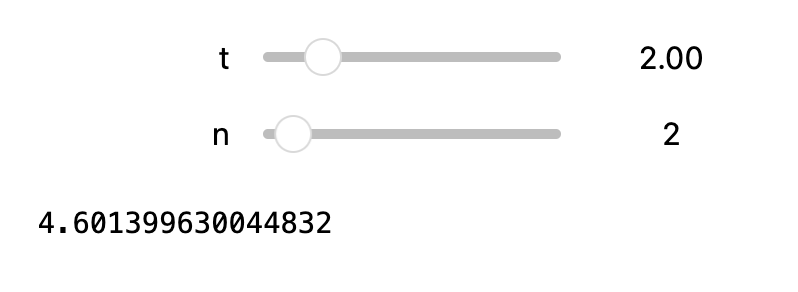
\includegraphics{screenshots/classes_1.png}
\caption{Widget screenshot}
\end{figure}

    \subsection*{1.5.2 Табуляція многочленів
Лаґерра}\label{ux442ux430ux431ux443ux43bux44fux446ux456ux44f-ux43cux43dux43eux433ux43eux447ux43bux435ux43dux456ux432-ux43bux430ux491ux435ux440ux440ux430}

Функція, що табулює многочлен Лаґерра порядку n від 0 до t\_max

    \begin{tcolorbox}[breakable, size=fbox, boxrule=1pt, pad at break*=1mm,colback=cellbackground, colframe=cellborder]
\prompt{In}{incolor}{12}{\boxspacing}
\begin{Verbatim}[commandchars=\\\{\}]
\PY{n}{ui}\PY{o}{.}\PY{n}{interactive\PYZus{}tabulate\PYZus{}polynomial}\PY{p}{(}\PY{p}{)}
\end{Verbatim}
\end{tcolorbox}

    
    \begin{Verbatim}[commandchars=\\\{\}]
interactive(children=(IntSlider(value=2, description='n', max=20), FloatSlider(value=5.0, description='Макс. t…
    \end{Verbatim}

    
            \begin{tcolorbox}[breakable, size=fbox, boxrule=.5pt, pad at break*=1mm, opacityfill=0]
\prompt{Out}{outcolor}{12}{\boxspacing}
\begin{Verbatim}[commandchars=\\\{\}]
<function ipywidgets.widgets.interaction.\_InteractFactory.\_\_call\_\_.<locals>.<lam
bda>(*args, **kwargs)>
\end{Verbatim}
\end{tcolorbox}
        
    \begin{figure}
\centering
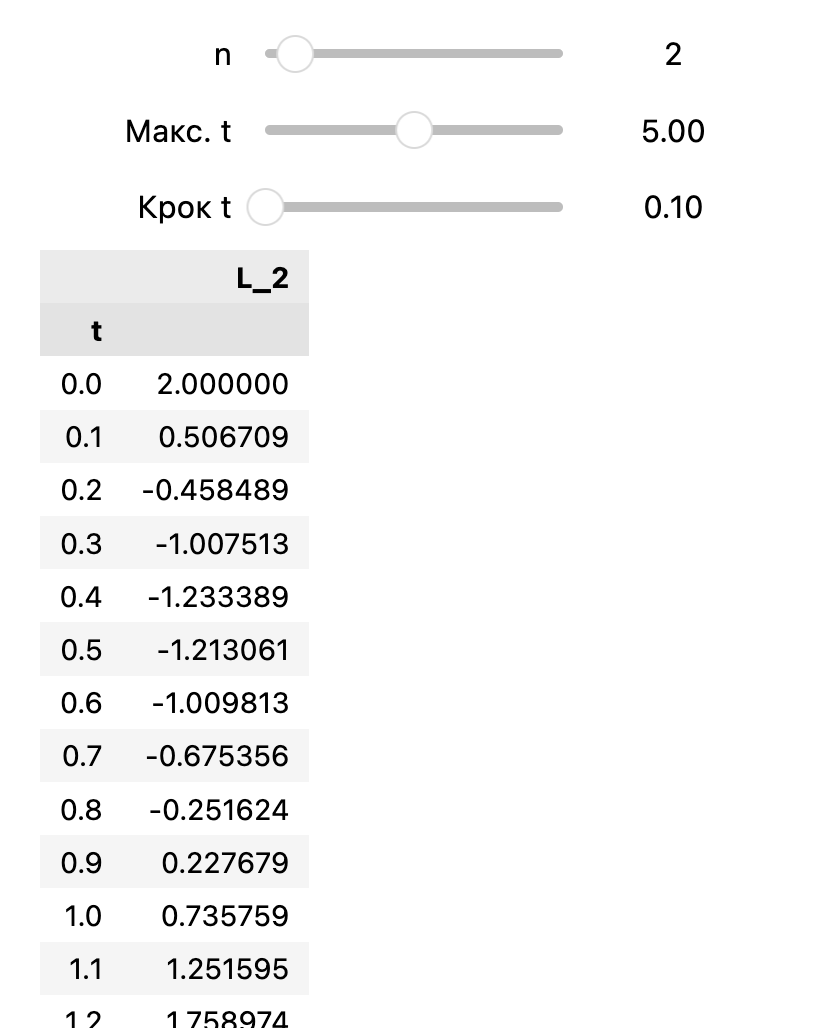
\includegraphics{screenshots/classes_2.png}
\caption{Widget screenshot}
\end{figure}

    \subsection*{1.5.3 Обчислювальний
експеримент}\label{ux43eux431ux447ux438ux441ux43bux44eux432ux430ux43bux44cux43dux438ux439-ux435ux43aux441ux43fux435ux440ux438ux43cux435ux43dux442}

Функція, що визначає найменше значення аргументу t, при якому всі
поліноми Лаґерра порядку від 0 до n\_max --- менші за epsilon

    \begin{tcolorbox}[breakable, size=fbox, boxrule=1pt, pad at break*=1mm,colback=cellbackground, colframe=cellborder]
\prompt{In}{incolor}{13}{\boxspacing}
\begin{Verbatim}[commandchars=\\\{\}]
\PY{n}{t}\PY{p}{,} \PY{n}{df} \PY{o}{=} \PY{n}{solver}\PY{o}{.}\PY{n}{find\PYZus{}optimal\PYZus{}t}\PY{p}{(}\PY{p}{)}

\PY{n+nb}{print}\PY{p}{(}\PY{l+s+sa}{f}\PY{l+s+s1}{\PYZsq{}}\PY{l+s+s1}{Оптимальне значення t: }\PY{l+s+si}{\PYZob{}}\PY{n}{t}\PY{l+s+si}{\PYZcb{}}\PY{l+s+s1}{\PYZsq{}}\PY{p}{)}
\PY{n}{df}
\end{Verbatim}
\end{tcolorbox}

    \begin{Verbatim}[commandchars=\\\{\}]
Оптимальне значення t: 79.07907907907908
    \end{Verbatim}

            \begin{tcolorbox}[breakable, size=fbox, boxrule=.5pt, pad at break*=1mm, opacityfill=0]
\prompt{Out}{outcolor}{13}{\boxspacing}
\begin{Verbatim}[commandchars=\\\{\}]
             L\_n
n
0   9.066138e-35
1  -2.858701e-32
2   4.478343e-30
3  -4.647081e-28
4   3.593209e-26
5  -2.208132e-24
6   1.123332e-22
7  -4.865604e-21
8   1.831625e-19
9  -6.087176e-18
10  1.808168e-16
11 -4.848845e-15
12  1.183547e-13
13 -2.647728e-12
14  5.460659e-11
15 -1.043487e-09
16  1.855654e-08
17 -3.082750e-07
18  4.800407e-06
19 -7.027805e-05
20  9.699021e-04
\end{Verbatim}
\end{tcolorbox}
        
    \subsection*{1.5.4 Обчислення значень
інтегралів}\label{ux43eux431ux447ux438ux441ux43bux435ux43dux43dux44f-ux437ux43dux430ux447ux435ux43dux44c-ux456ux43dux442ux435ux433ux440ux430ux43bux456ux432}

Функція для обчислення прямого перетворення Лаґерра за допомогою
апроксимації інтегралу методом прямокутників

    \begin{tcolorbox}[breakable, size=fbox, boxrule=1pt, pad at break*=1mm,colback=cellbackground, colframe=cellborder]
\prompt{In}{incolor}{14}{\boxspacing}
\begin{Verbatim}[commandchars=\\\{\}]
\PY{n}{ui}\PY{o}{.}\PY{n}{interactive\PYZus{}solve\PYZus{}laguerre\PYZus{}transform}\PY{p}{(}\PY{k}{lambda} \PY{n}{t}\PY{p}{:} \PY{n}{np}\PY{o}{.}\PY{n}{exp}\PY{p}{(}\PY{o}{\PYZhy{}}\PY{n}{t} \PY{o}{*}\PY{o}{*} \PY{l+m+mi}{2}\PY{p}{)}\PY{p}{)}
\end{Verbatim}
\end{tcolorbox}

    
    \begin{Verbatim}[commandchars=\\\{\}]
interactive(children=(IntSlider(value=20, description='Макс. n', max=20), IntSlider(value=10000, description='…
    \end{Verbatim}

    
            \begin{tcolorbox}[breakable, size=fbox, boxrule=.5pt, pad at break*=1mm, opacityfill=0]
\prompt{Out}{outcolor}{14}{\boxspacing}
\begin{Verbatim}[commandchars=\\\{\}]
<function ipywidgets.widgets.interaction.\_InteractFactory.\_\_call\_\_.<locals>.<lam
bda>(*args, **kwargs)>
\end{Verbatim}
\end{tcolorbox}
        
    \begin{figure}
\centering
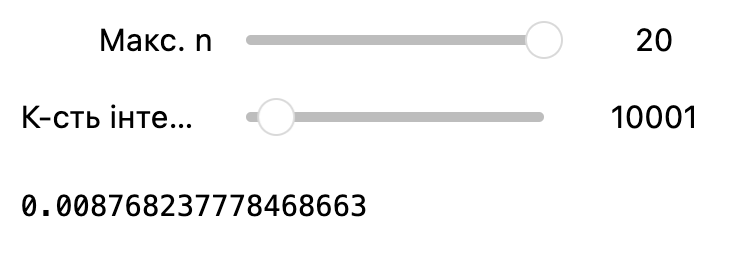
\includegraphics{screenshots/classes_3.png}
\caption{Widget screenshot}
\end{figure}

    \subsection*{1.5.5 Перетворення
Лаґерра}\label{ux43fux435ux440ux435ux442ux432ux43eux440ux435ux43dux43dux44f-ux43bux430ux491ux435ux440ux440ux430}

Функція для табулювання прямого перетворення Лаґерра порядку від 0 до
n\_max

    \begin{tcolorbox}[breakable, size=fbox, boxrule=1pt, pad at break*=1mm,colback=cellbackground, colframe=cellborder]
\prompt{In}{incolor}{15}{\boxspacing}
\begin{Verbatim}[commandchars=\\\{\}]
\PY{c+c1}{\PYZsh{} Табулювання}
\PY{n}{ui}\PY{o}{.}\PY{n}{interactive\PYZus{}tabulate\PYZus{}laguerre\PYZus{}transform}\PY{p}{(}\PY{n}{f\PYZus{}1}\PY{p}{)}
\end{Verbatim}
\end{tcolorbox}

    
    \begin{Verbatim}[commandchars=\\\{\}]
interactive(children=(IntSlider(value=20, description='Макс. n', max=20), IntSlider(value=10000, description='…
    \end{Verbatim}

    
            \begin{tcolorbox}[breakable, size=fbox, boxrule=.5pt, pad at break*=1mm, opacityfill=0]
\prompt{Out}{outcolor}{15}{\boxspacing}
\begin{Verbatim}[commandchars=\\\{\}]
<function ipywidgets.widgets.interaction.\_InteractFactory.\_\_call\_\_.<locals>.<lam
bda>(*args, **kwargs)>
\end{Verbatim}
\end{tcolorbox}
        
    \begin{figure}
\centering
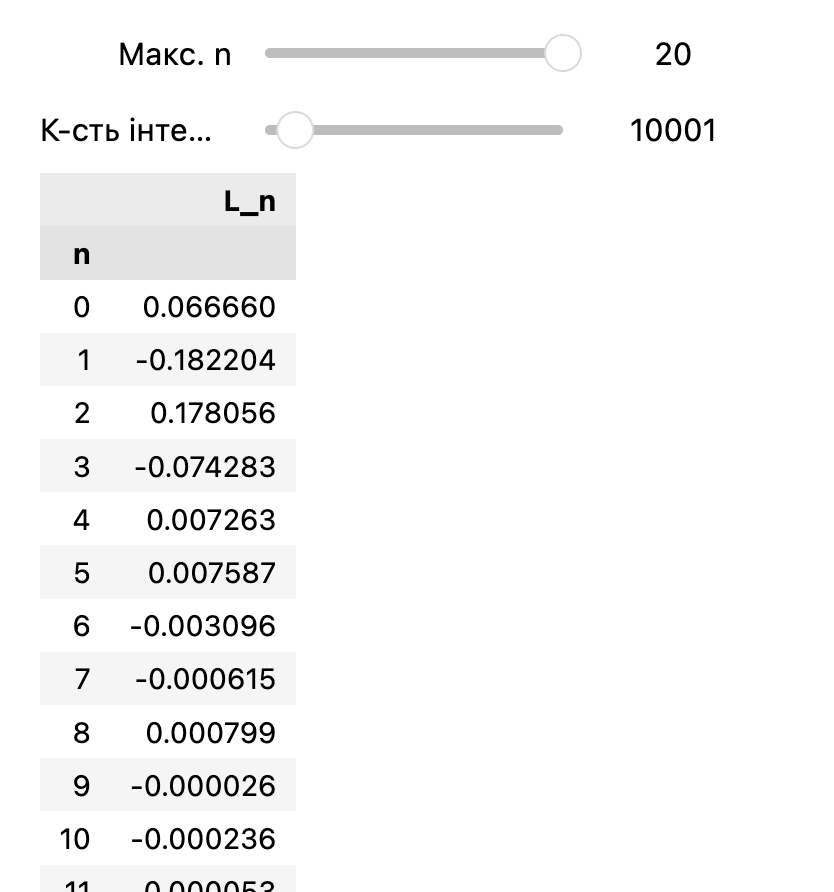
\includegraphics{screenshots/classes_4.png}
\caption{Widget screenshot}
\end{figure}

    \subsection*{1.5.6 Обернене перетворення
Лаґерра}\label{ux43eux431ux435ux440ux43dux435ux43dux435-ux43fux435ux440ux435ux442ux432ux43eux440ux435ux43dux43dux44f-ux43bux430ux491ux435ux440ux440ux430}

Функція для обчислення оберненого перетворення Лаґерра. Приймає
послідовність коєфіцієнтів h, які можна отримати з табуляції
перетворення Лаґерра

    \begin{tcolorbox}[breakable, size=fbox, boxrule=1pt, pad at break*=1mm,colback=cellbackground, colframe=cellborder]
\prompt{In}{incolor}{16}{\boxspacing}
\begin{Verbatim}[commandchars=\\\{\}]
\PY{c+c1}{\PYZsh{} Отримуємо послідовність h з табуляції перетворення Лаґерра}
\PY{n}{h} \PY{o}{=} \PY{n}{solver}\PY{o}{.}\PY{n}{tabulate\PYZus{}laguerre\PYZus{}transform}\PY{p}{(}
    \PY{n}{f}\PY{o}{=}\PY{n}{f\PYZus{}1}\PY{p}{,}
    \PY{n}{n\PYZus{}max}\PY{o}{=}\PY{l+m+mi}{20}\PY{p}{,}
    \PY{n}{int\PYZus{}points}\PY{o}{=}\PY{l+m+mi}{10000}
\PY{p}{)}\PY{p}{[}\PY{l+s+s1}{\PYZsq{}}\PY{l+s+s1}{L\PYZus{}n}\PY{l+s+s1}{\PYZsq{}}\PY{p}{]}\PY{o}{.}\PY{n}{tolist}\PY{p}{(}\PY{p}{)}

\PY{n}{ui}\PY{o}{.}\PY{n}{interactive\PYZus{}solve\PYZus{}inverse\PYZus{}laguerre\PYZus{}transform}\PY{p}{(}\PY{n}{h}\PY{p}{)}
\end{Verbatim}
\end{tcolorbox}

    
    \begin{Verbatim}[commandchars=\\\{\}]
interactive(children=(FloatSlider(value=2.0, description='t', max=10.0), Output()), \_dom\_classes=('widget-inte…
    \end{Verbatim}

    
            \begin{tcolorbox}[breakable, size=fbox, boxrule=.5pt, pad at break*=1mm, opacityfill=0]
\prompt{Out}{outcolor}{16}{\boxspacing}
\begin{Verbatim}[commandchars=\\\{\}]
<function ipywidgets.widgets.interaction.\_InteractFactory.\_\_call\_\_.<locals>.<lam
bda>(*args, **kwargs)>
\end{Verbatim}
\end{tcolorbox}
        
    \begin{figure}
\centering
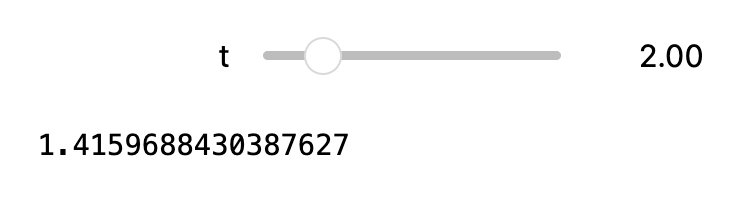
\includegraphics{screenshots/classes_5.png}
\caption{Widget screenshot}
\end{figure}

    \subsection*{1.5.7 Графік функції
Лаґерра}\label{ux433ux440ux430ux444ux456ux43a-ux444ux443ux43dux43aux446ux456ux457-ux43bux430ux491ux435ux440ux440ux430}

Функція для побудови графіку многочленів Лаґерра порядку від 0 до n\_max

    \begin{tcolorbox}[breakable, size=fbox, boxrule=1pt, pad at break*=1mm,colback=cellbackground, colframe=cellborder]
\prompt{In}{incolor}{17}{\boxspacing}
\begin{Verbatim}[commandchars=\\\{\}]
\PY{n}{ui}\PY{o}{.}\PY{n}{interactive\PYZus{}plot\PYZus{}laguerre\PYZus{}polynomials}\PY{p}{(}\PY{p}{)}
\end{Verbatim}
\end{tcolorbox}

    
    \begin{Verbatim}[commandchars=\\\{\}]
interactive(children=(FloatSlider(value=10.0, description='Макс. t', max=20.0), IntSlider(value=20, descriptio…
    \end{Verbatim}

    
            \begin{tcolorbox}[breakable, size=fbox, boxrule=.5pt, pad at break*=1mm, opacityfill=0]
\prompt{Out}{outcolor}{17}{\boxspacing}
\begin{Verbatim}[commandchars=\\\{\}]
<function ipywidgets.widgets.interaction.\_InteractFactory.\_\_call\_\_.<locals>.<lam
bda>(*args, **kwargs)>
\end{Verbatim}
\end{tcolorbox}
        
    \begin{figure}
\centering
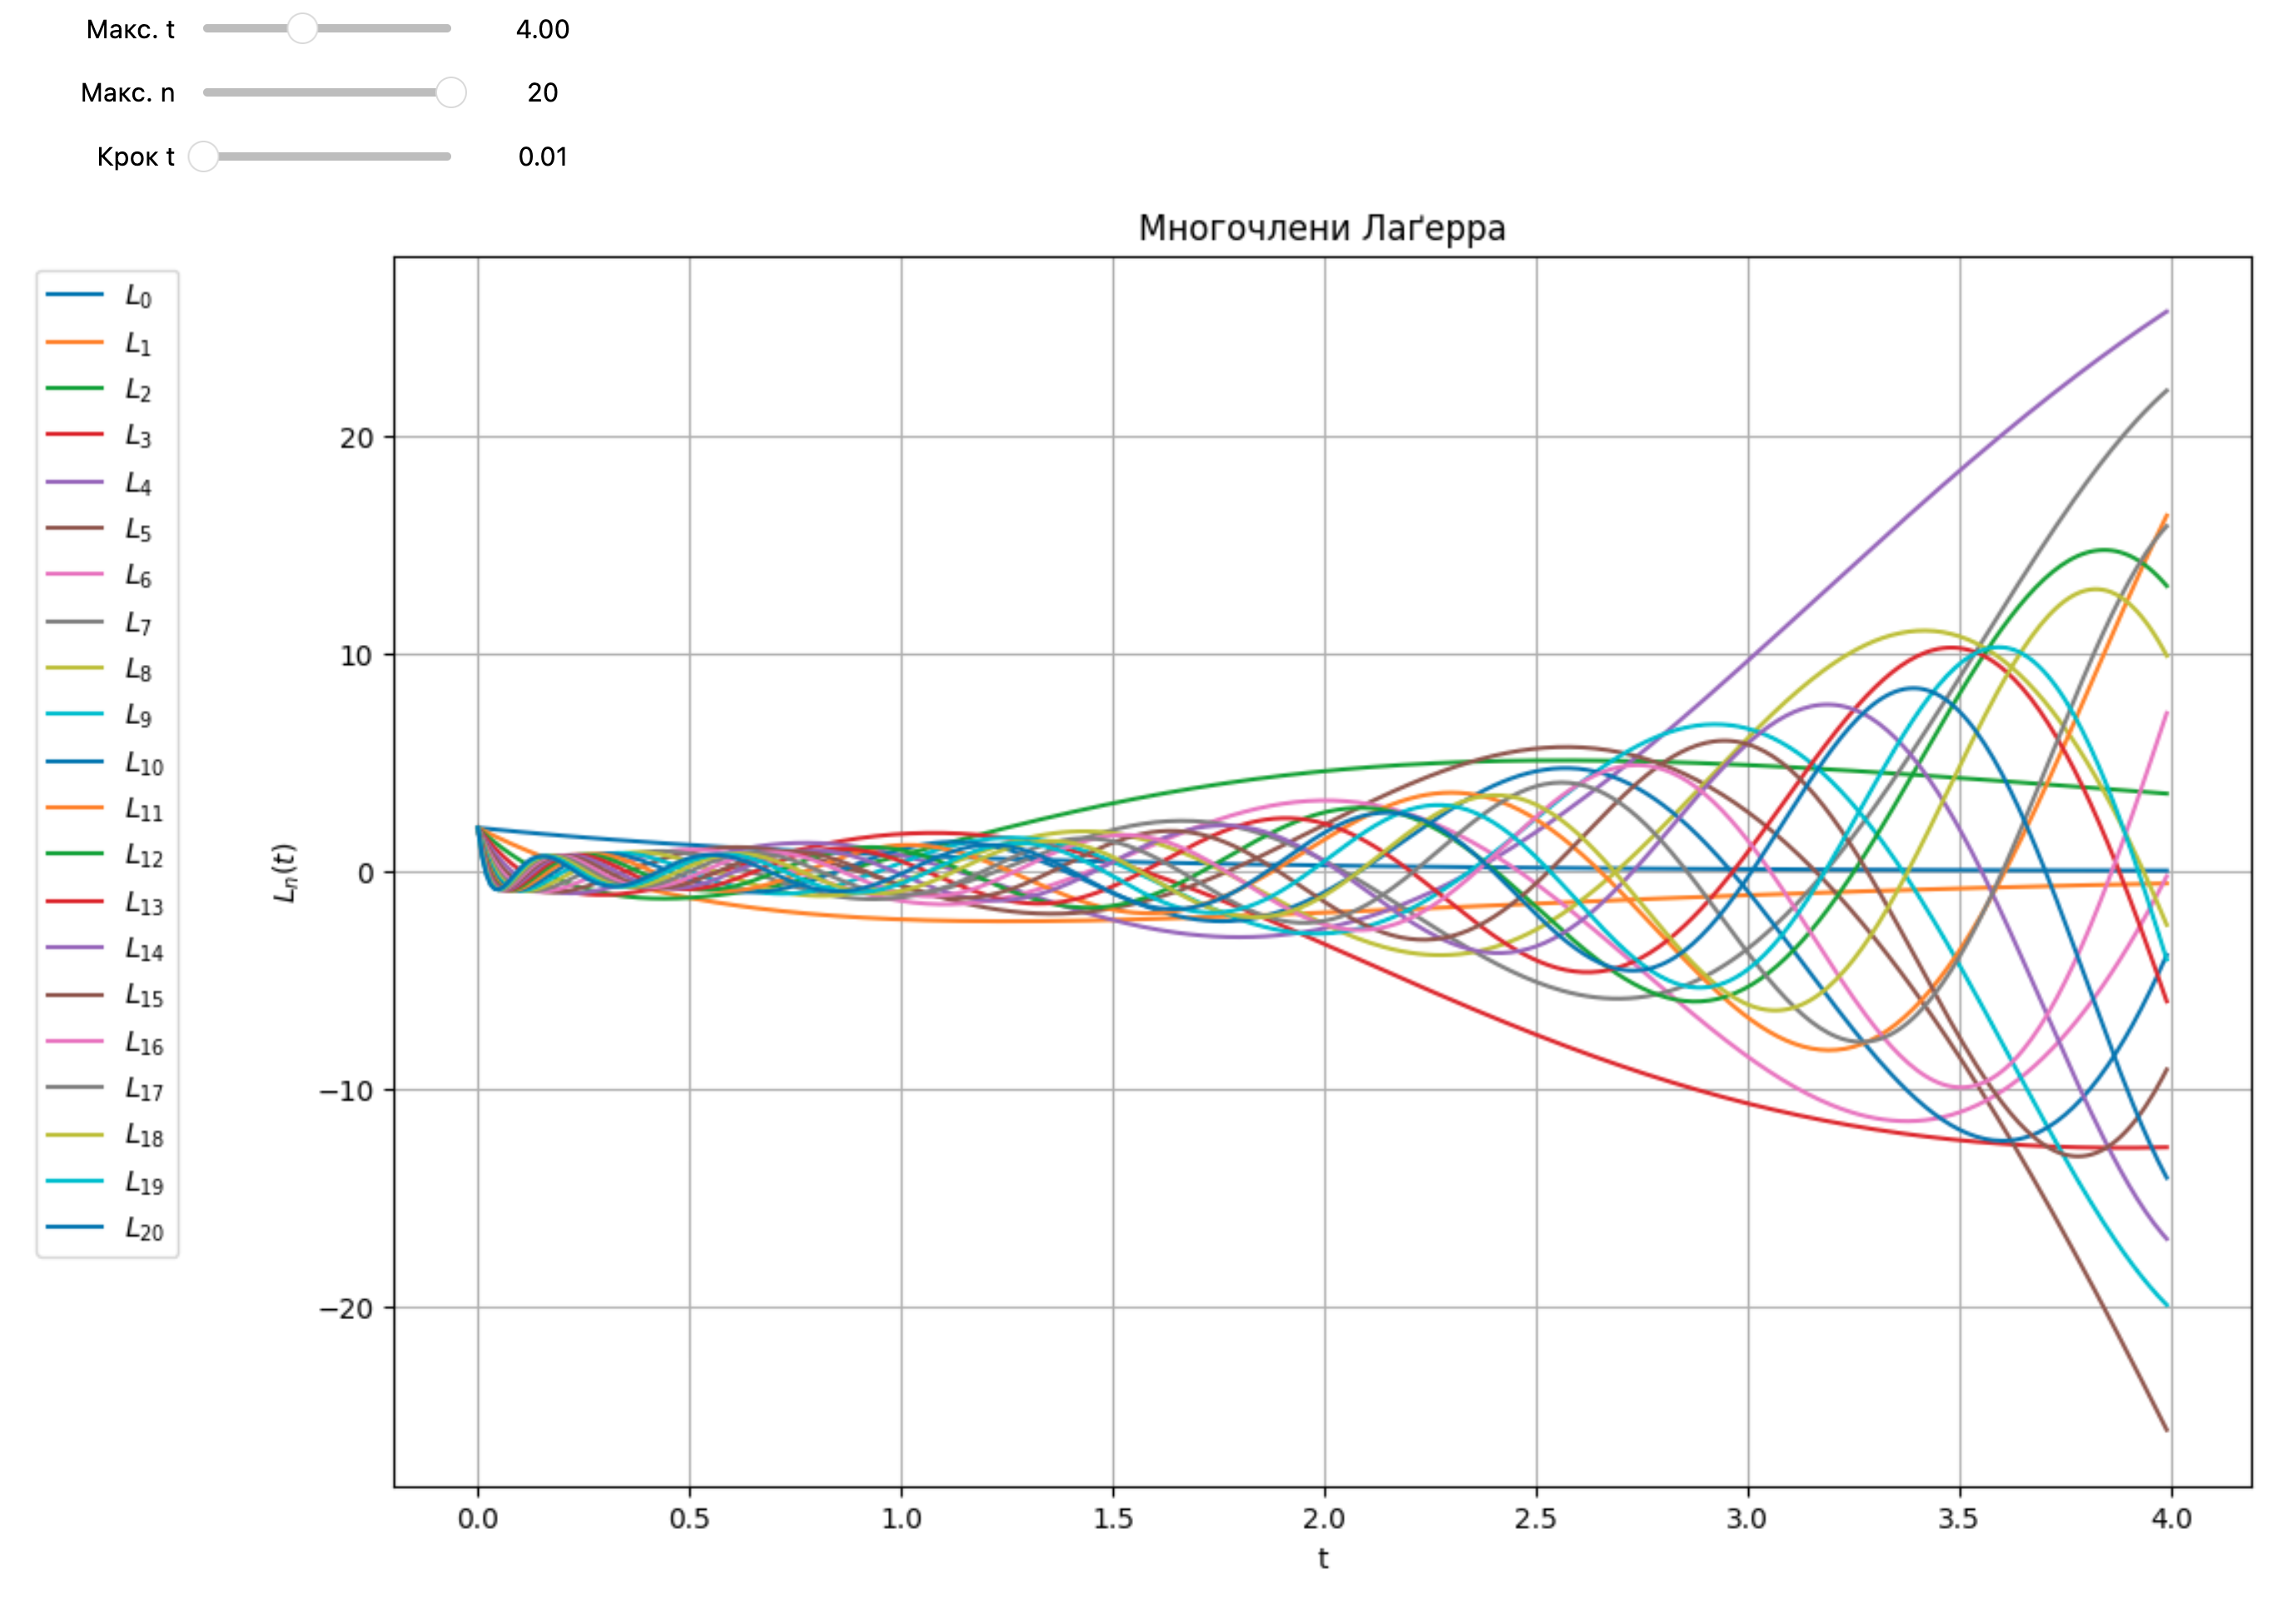
\includegraphics{screenshots/classes_6.png}
\caption{Widget screenshot}
\end{figure}

    \subsection*{\texorpdfstring{1.5.8 Графік
\(\widetilde{f_1}^N(t)\)}{1.5.8 Графік \textbackslash widetilde\{f\_1\}\^{}N(t)}}\label{ux433ux440ux430ux444ux456ux43a-widetildef_1nt}

    \begin{tcolorbox}[breakable, size=fbox, boxrule=1pt, pad at break*=1mm,colback=cellbackground, colframe=cellborder]
\prompt{In}{incolor}{18}{\boxspacing}
\begin{Verbatim}[commandchars=\\\{\}]
\PY{n}{ui}\PY{o}{.}\PY{n}{interactive\PYZus{}plot\PYZus{}laguerre\PYZus{}transform}\PY{p}{(}\PY{n}{f\PYZus{}1}\PY{p}{)}
\end{Verbatim}
\end{tcolorbox}

    
    \begin{Verbatim}[commandchars=\\\{\}]
interactive(children=(IntSlider(value=20, description='Макс. n', max=20), FloatSlider(value=10.0, description=…
    \end{Verbatim}

    
            \begin{tcolorbox}[breakable, size=fbox, boxrule=.5pt, pad at break*=1mm, opacityfill=0]
\prompt{Out}{outcolor}{18}{\boxspacing}
\begin{Verbatim}[commandchars=\\\{\}]
<function ipywidgets.widgets.interaction.\_InteractFactory.\_\_call\_\_.<locals>.<lam
bda>(*args, **kwargs)>
\end{Verbatim}
\end{tcolorbox}
        
    \begin{figure}
\centering
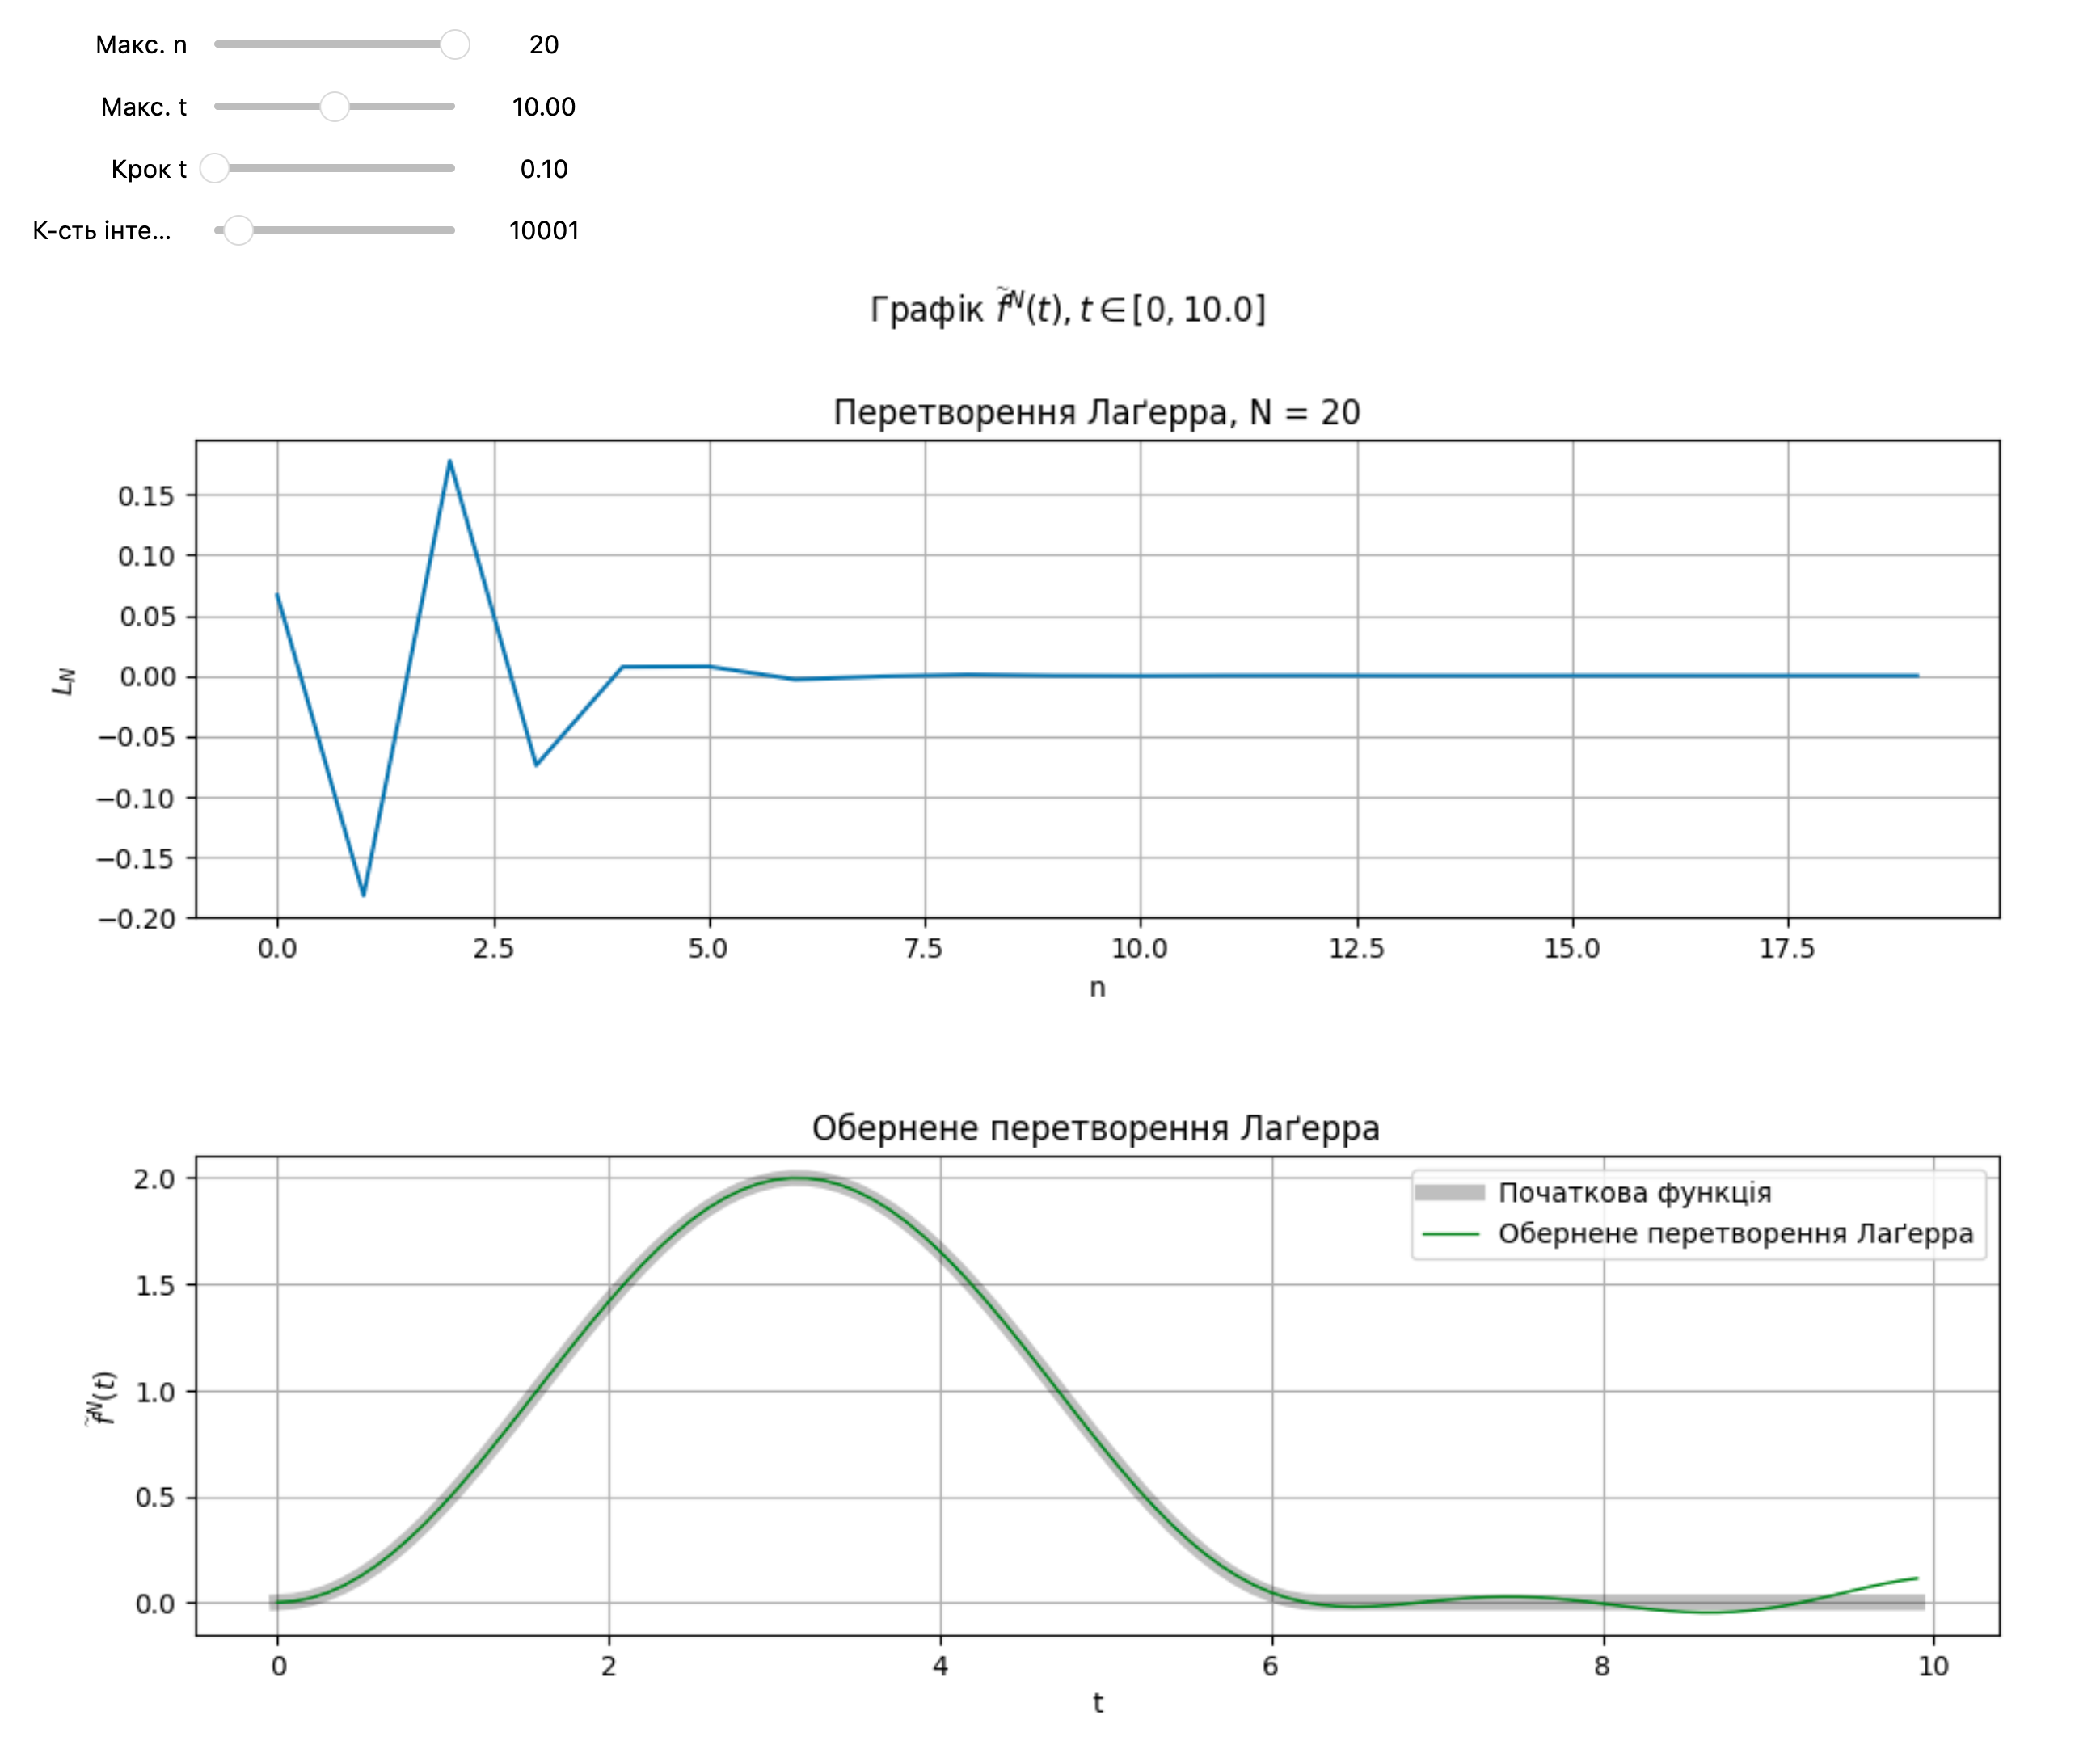
\includegraphics{screenshots/classes_7.png}
\caption{Widget screenshot}
\end{figure}

    \subsection*{\texorpdfstring{Графік
\(\widetilde{f_2}^N(t)\)}{Графік \textbackslash widetilde\{f\_2\}\^{}N(t)}}\label{ux433ux440ux430ux444ux456ux43a-widetildef_2nt}

    \begin{tcolorbox}[breakable, size=fbox, boxrule=1pt, pad at break*=1mm,colback=cellbackground, colframe=cellborder]
\prompt{In}{incolor}{19}{\boxspacing}
\begin{Verbatim}[commandchars=\\\{\}]
\PY{n}{ui}\PY{o}{.}\PY{n}{interactive\PYZus{}plot\PYZus{}laguerre\PYZus{}transform}\PY{p}{(}\PY{n}{f\PYZus{}2}\PY{p}{)}
\end{Verbatim}
\end{tcolorbox}

    
    \begin{Verbatim}[commandchars=\\\{\}]
interactive(children=(IntSlider(value=20, description='Макс. n', max=20), FloatSlider(value=10.0, description=…
    \end{Verbatim}

    
            \begin{tcolorbox}[breakable, size=fbox, boxrule=.5pt, pad at break*=1mm, opacityfill=0]
\prompt{Out}{outcolor}{19}{\boxspacing}
\begin{Verbatim}[commandchars=\\\{\}]
<function ipywidgets.widgets.interaction.\_InteractFactory.\_\_call\_\_.<locals>.<lam
bda>(*args, **kwargs)>
\end{Verbatim}
\end{tcolorbox}
        
    \begin{figure}
\centering
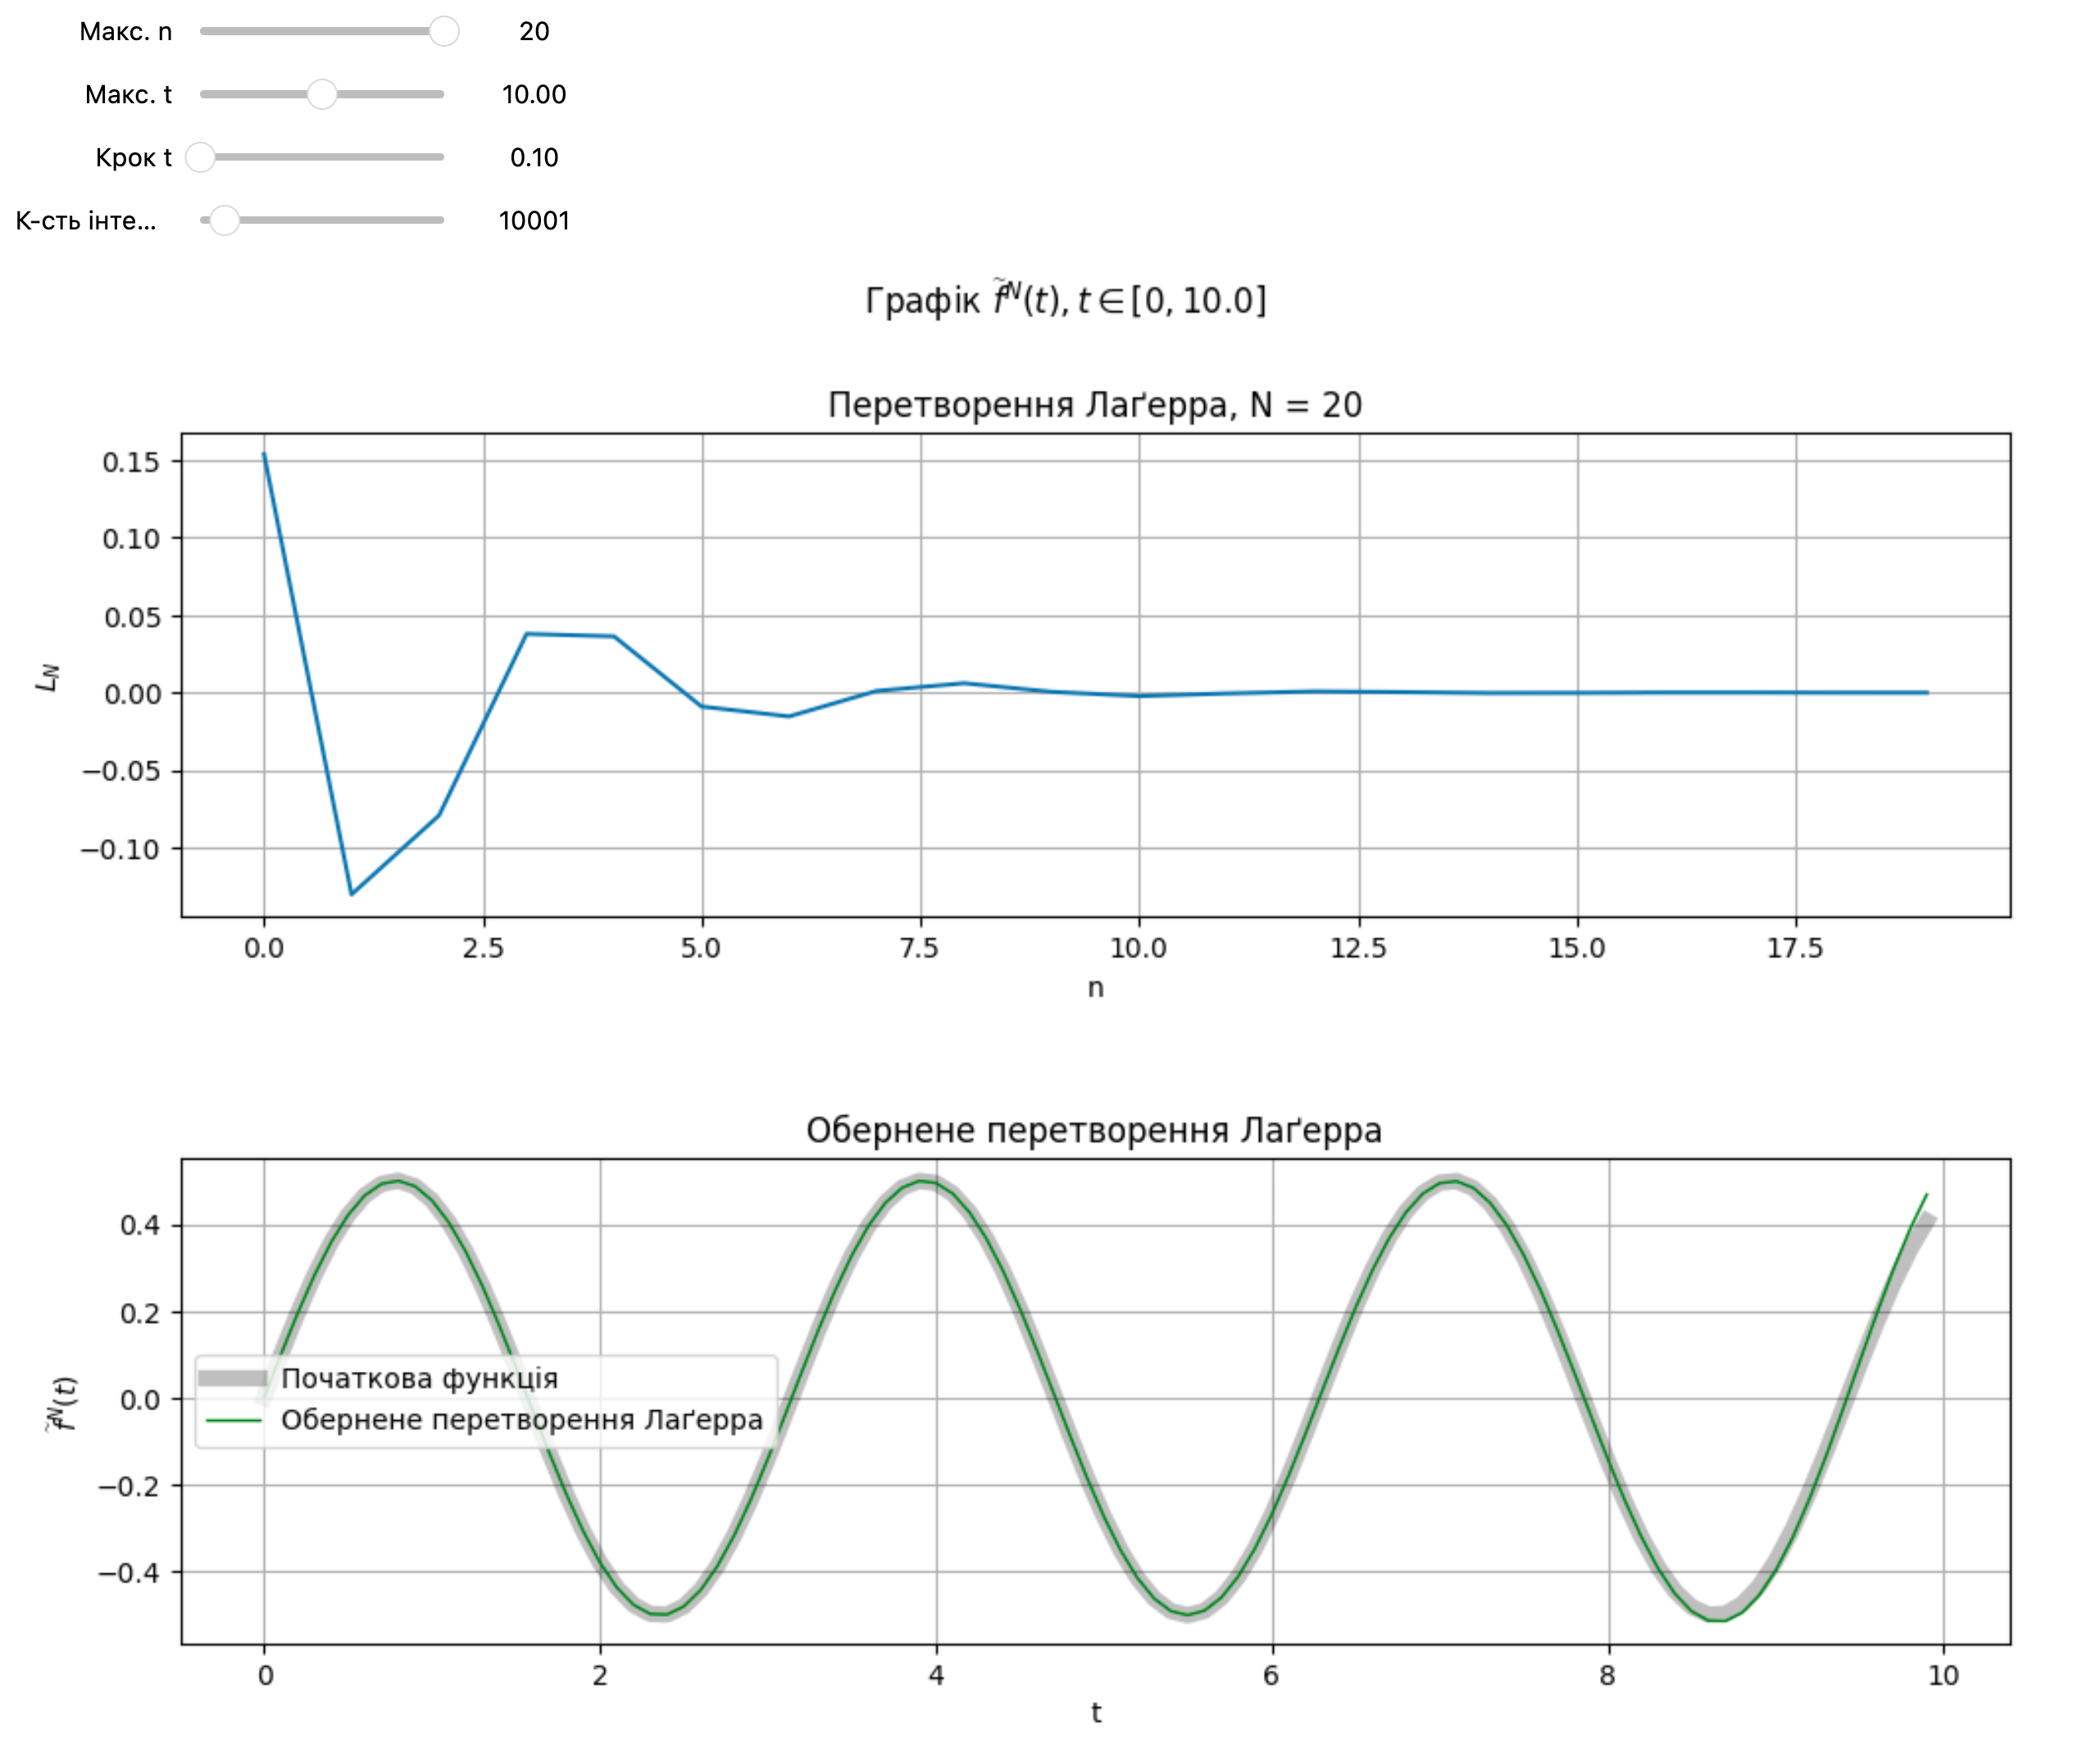
\includegraphics{screenshots/classes_8.png}
\caption{Widget screenshot}
\end{figure}

    \subsection*{\texorpdfstring{Графік
\(\widetilde{f_3}^N(t)\)}{Графік \textbackslash widetilde\{f\_3\}\^{}N(t)}}\label{ux433ux440ux430ux444ux456ux43a-widetildef_3nt}

    \begin{tcolorbox}[breakable, size=fbox, boxrule=1pt, pad at break*=1mm,colback=cellbackground, colframe=cellborder]
\prompt{In}{incolor}{20}{\boxspacing}
\begin{Verbatim}[commandchars=\\\{\}]
\PY{n}{ui}\PY{o}{.}\PY{n}{interactive\PYZus{}plot\PYZus{}laguerre\PYZus{}transform}\PY{p}{(}\PY{n}{f\PYZus{}3}\PY{p}{)}
\end{Verbatim}
\end{tcolorbox}

    
    \begin{Verbatim}[commandchars=\\\{\}]
interactive(children=(IntSlider(value=20, description='Макс. n', max=20), FloatSlider(value=10.0, description=…
    \end{Verbatim}

    
            \begin{tcolorbox}[breakable, size=fbox, boxrule=.5pt, pad at break*=1mm, opacityfill=0]
\prompt{Out}{outcolor}{20}{\boxspacing}
\begin{Verbatim}[commandchars=\\\{\}]
<function ipywidgets.widgets.interaction.\_InteractFactory.\_\_call\_\_.<locals>.<lam
bda>(*args, **kwargs)>
\end{Verbatim}
\end{tcolorbox}
        
    \begin{figure}
\centering
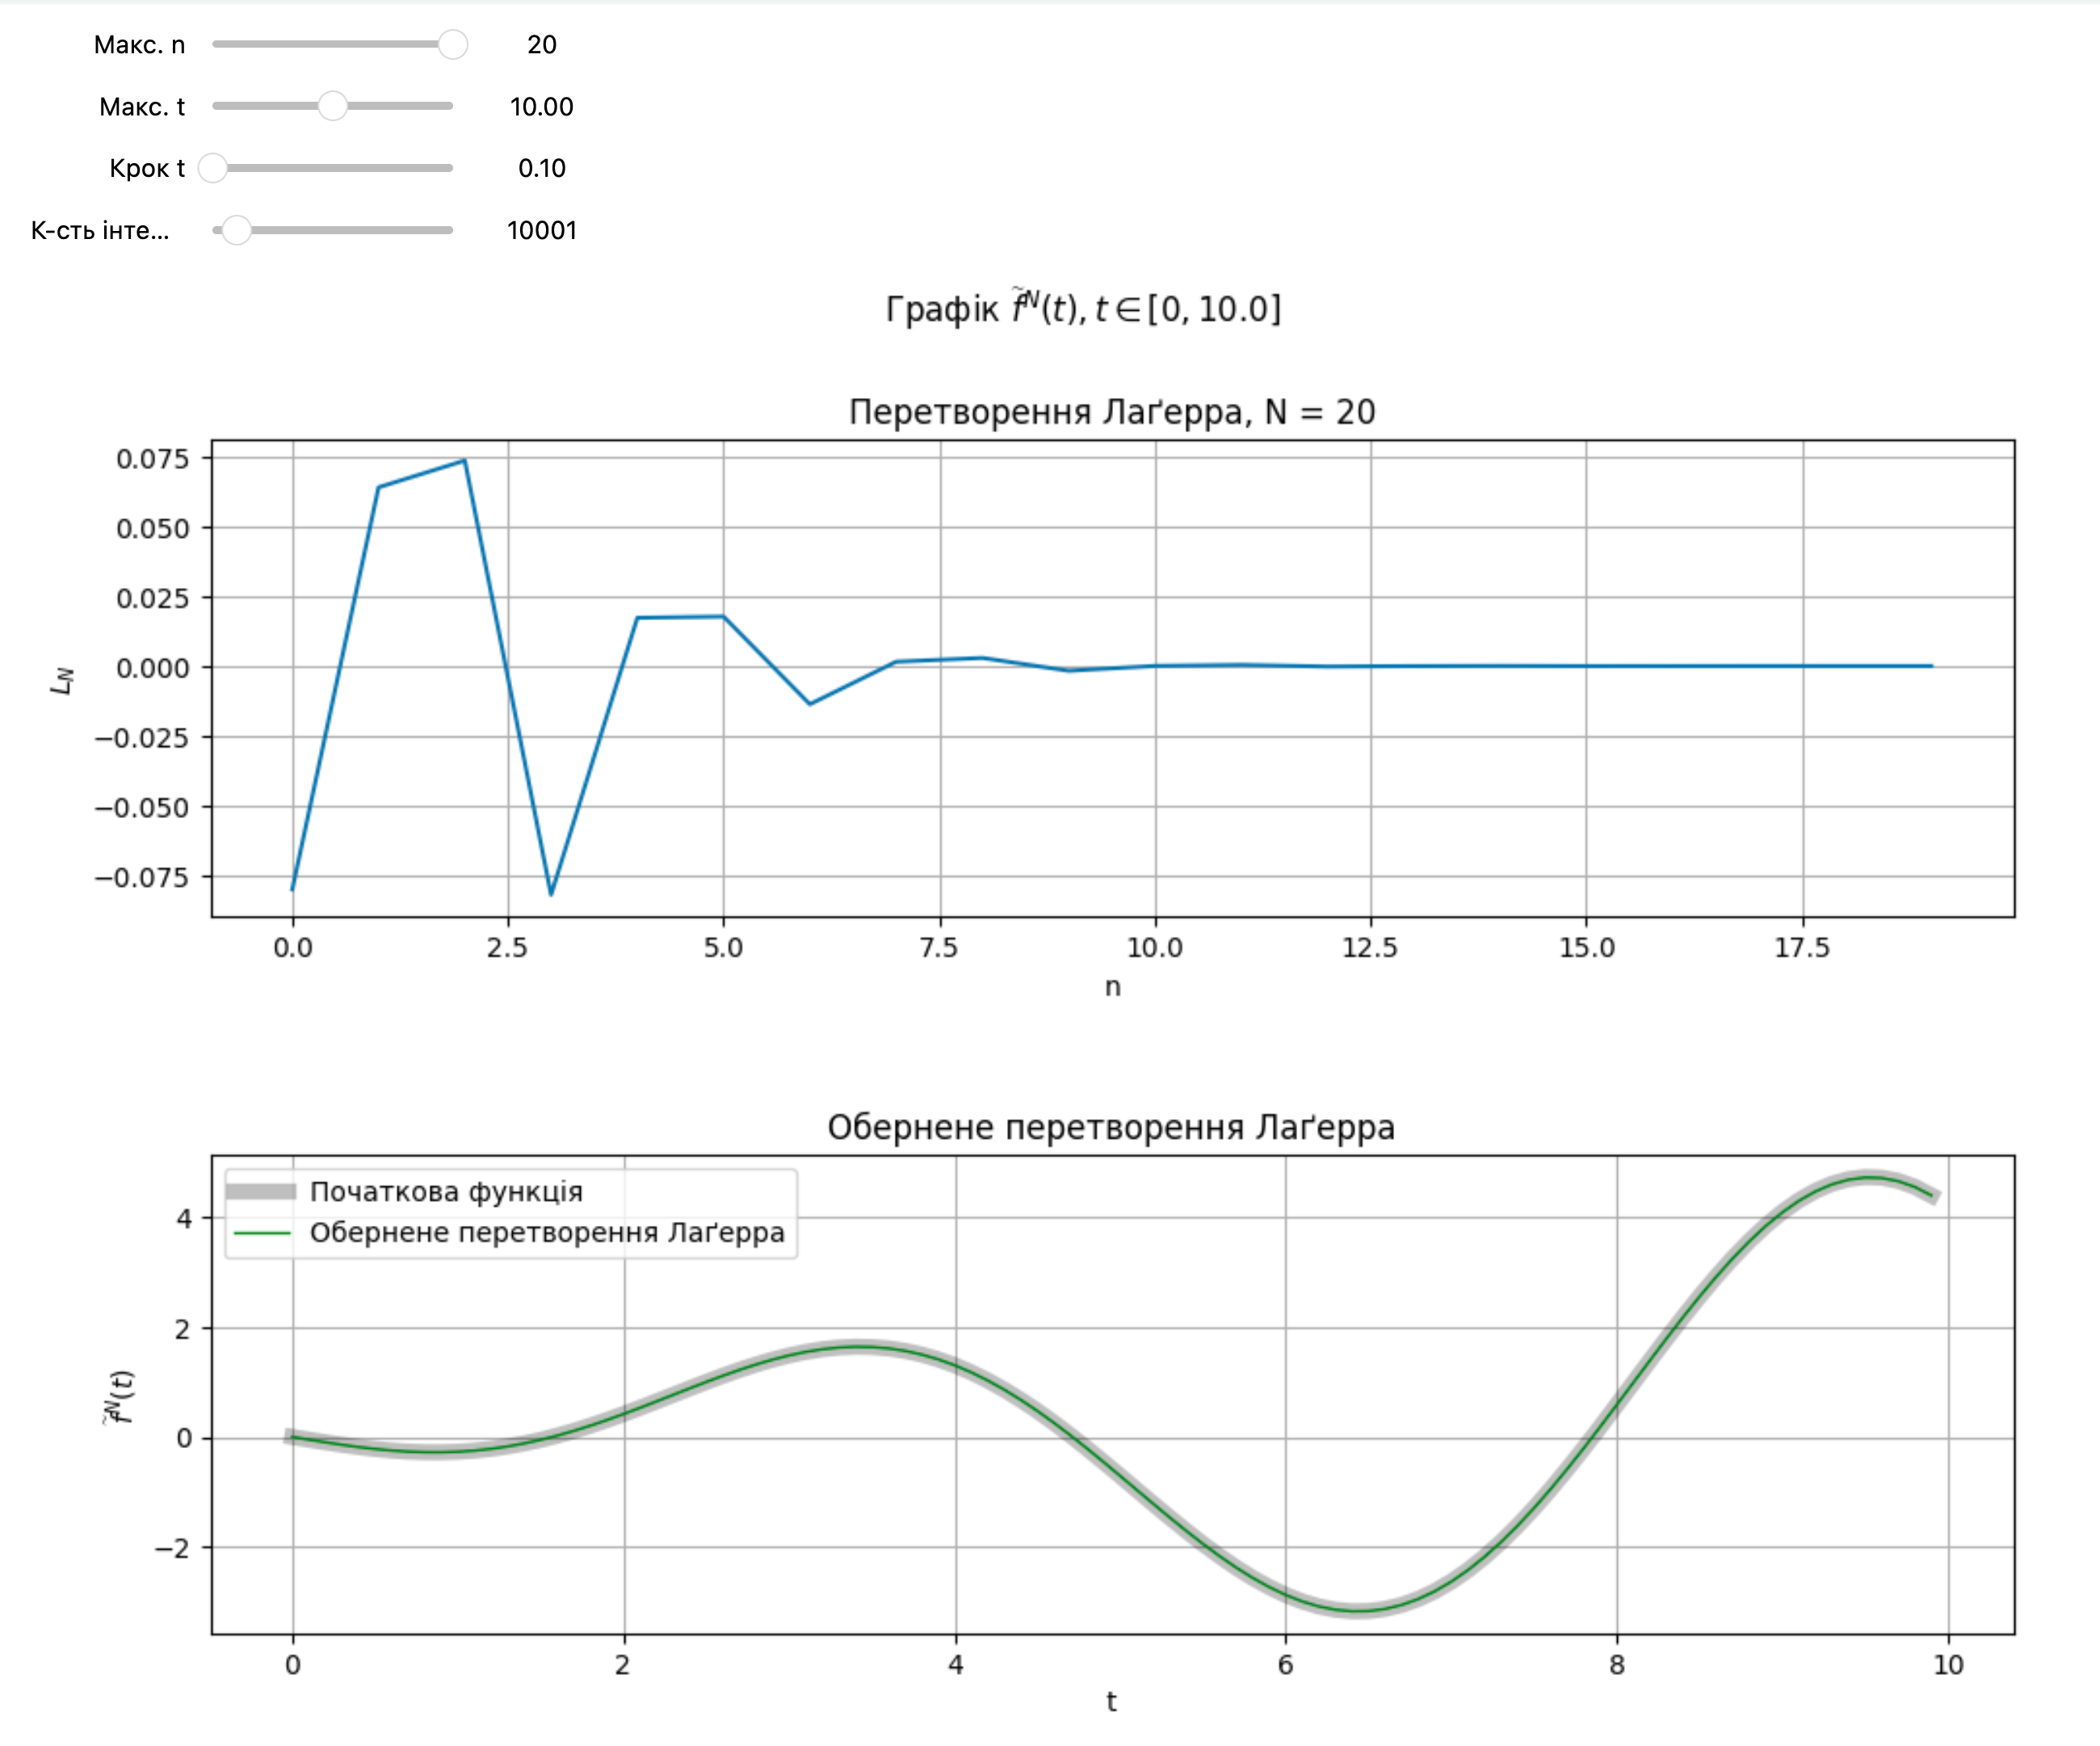
\includegraphics{screenshots/classes_9.png}
\caption{Widget screenshot}
\end{figure}

    \subsection*{\texorpdfstring{Графік
\(\widetilde{f_4}^N(t)\)}{Графік \textbackslash widetilde\{f\_4\}\^{}N(t)}}\label{ux433ux440ux430ux444ux456ux43a-widetildef_4nt}

    \begin{tcolorbox}[breakable, size=fbox, boxrule=1pt, pad at break*=1mm,colback=cellbackground, colframe=cellborder]
\prompt{In}{incolor}{21}{\boxspacing}
\begin{Verbatim}[commandchars=\\\{\}]
\PY{n}{ui}\PY{o}{.}\PY{n}{interactive\PYZus{}plot\PYZus{}laguerre\PYZus{}transform}\PY{p}{(}\PY{n}{f\PYZus{}4}\PY{p}{)}
\end{Verbatim}
\end{tcolorbox}

    
    \begin{Verbatim}[commandchars=\\\{\}]
interactive(children=(IntSlider(value=20, description='Макс. n', max=20), FloatSlider(value=10.0, description=…
    \end{Verbatim}

    
            \begin{tcolorbox}[breakable, size=fbox, boxrule=.5pt, pad at break*=1mm, opacityfill=0]
\prompt{Out}{outcolor}{21}{\boxspacing}
\begin{Verbatim}[commandchars=\\\{\}]
<function ipywidgets.widgets.interaction.\_InteractFactory.\_\_call\_\_.<locals>.<lam
bda>(*args, **kwargs)>
\end{Verbatim}
\end{tcolorbox}
        
    \begin{figure}
\centering
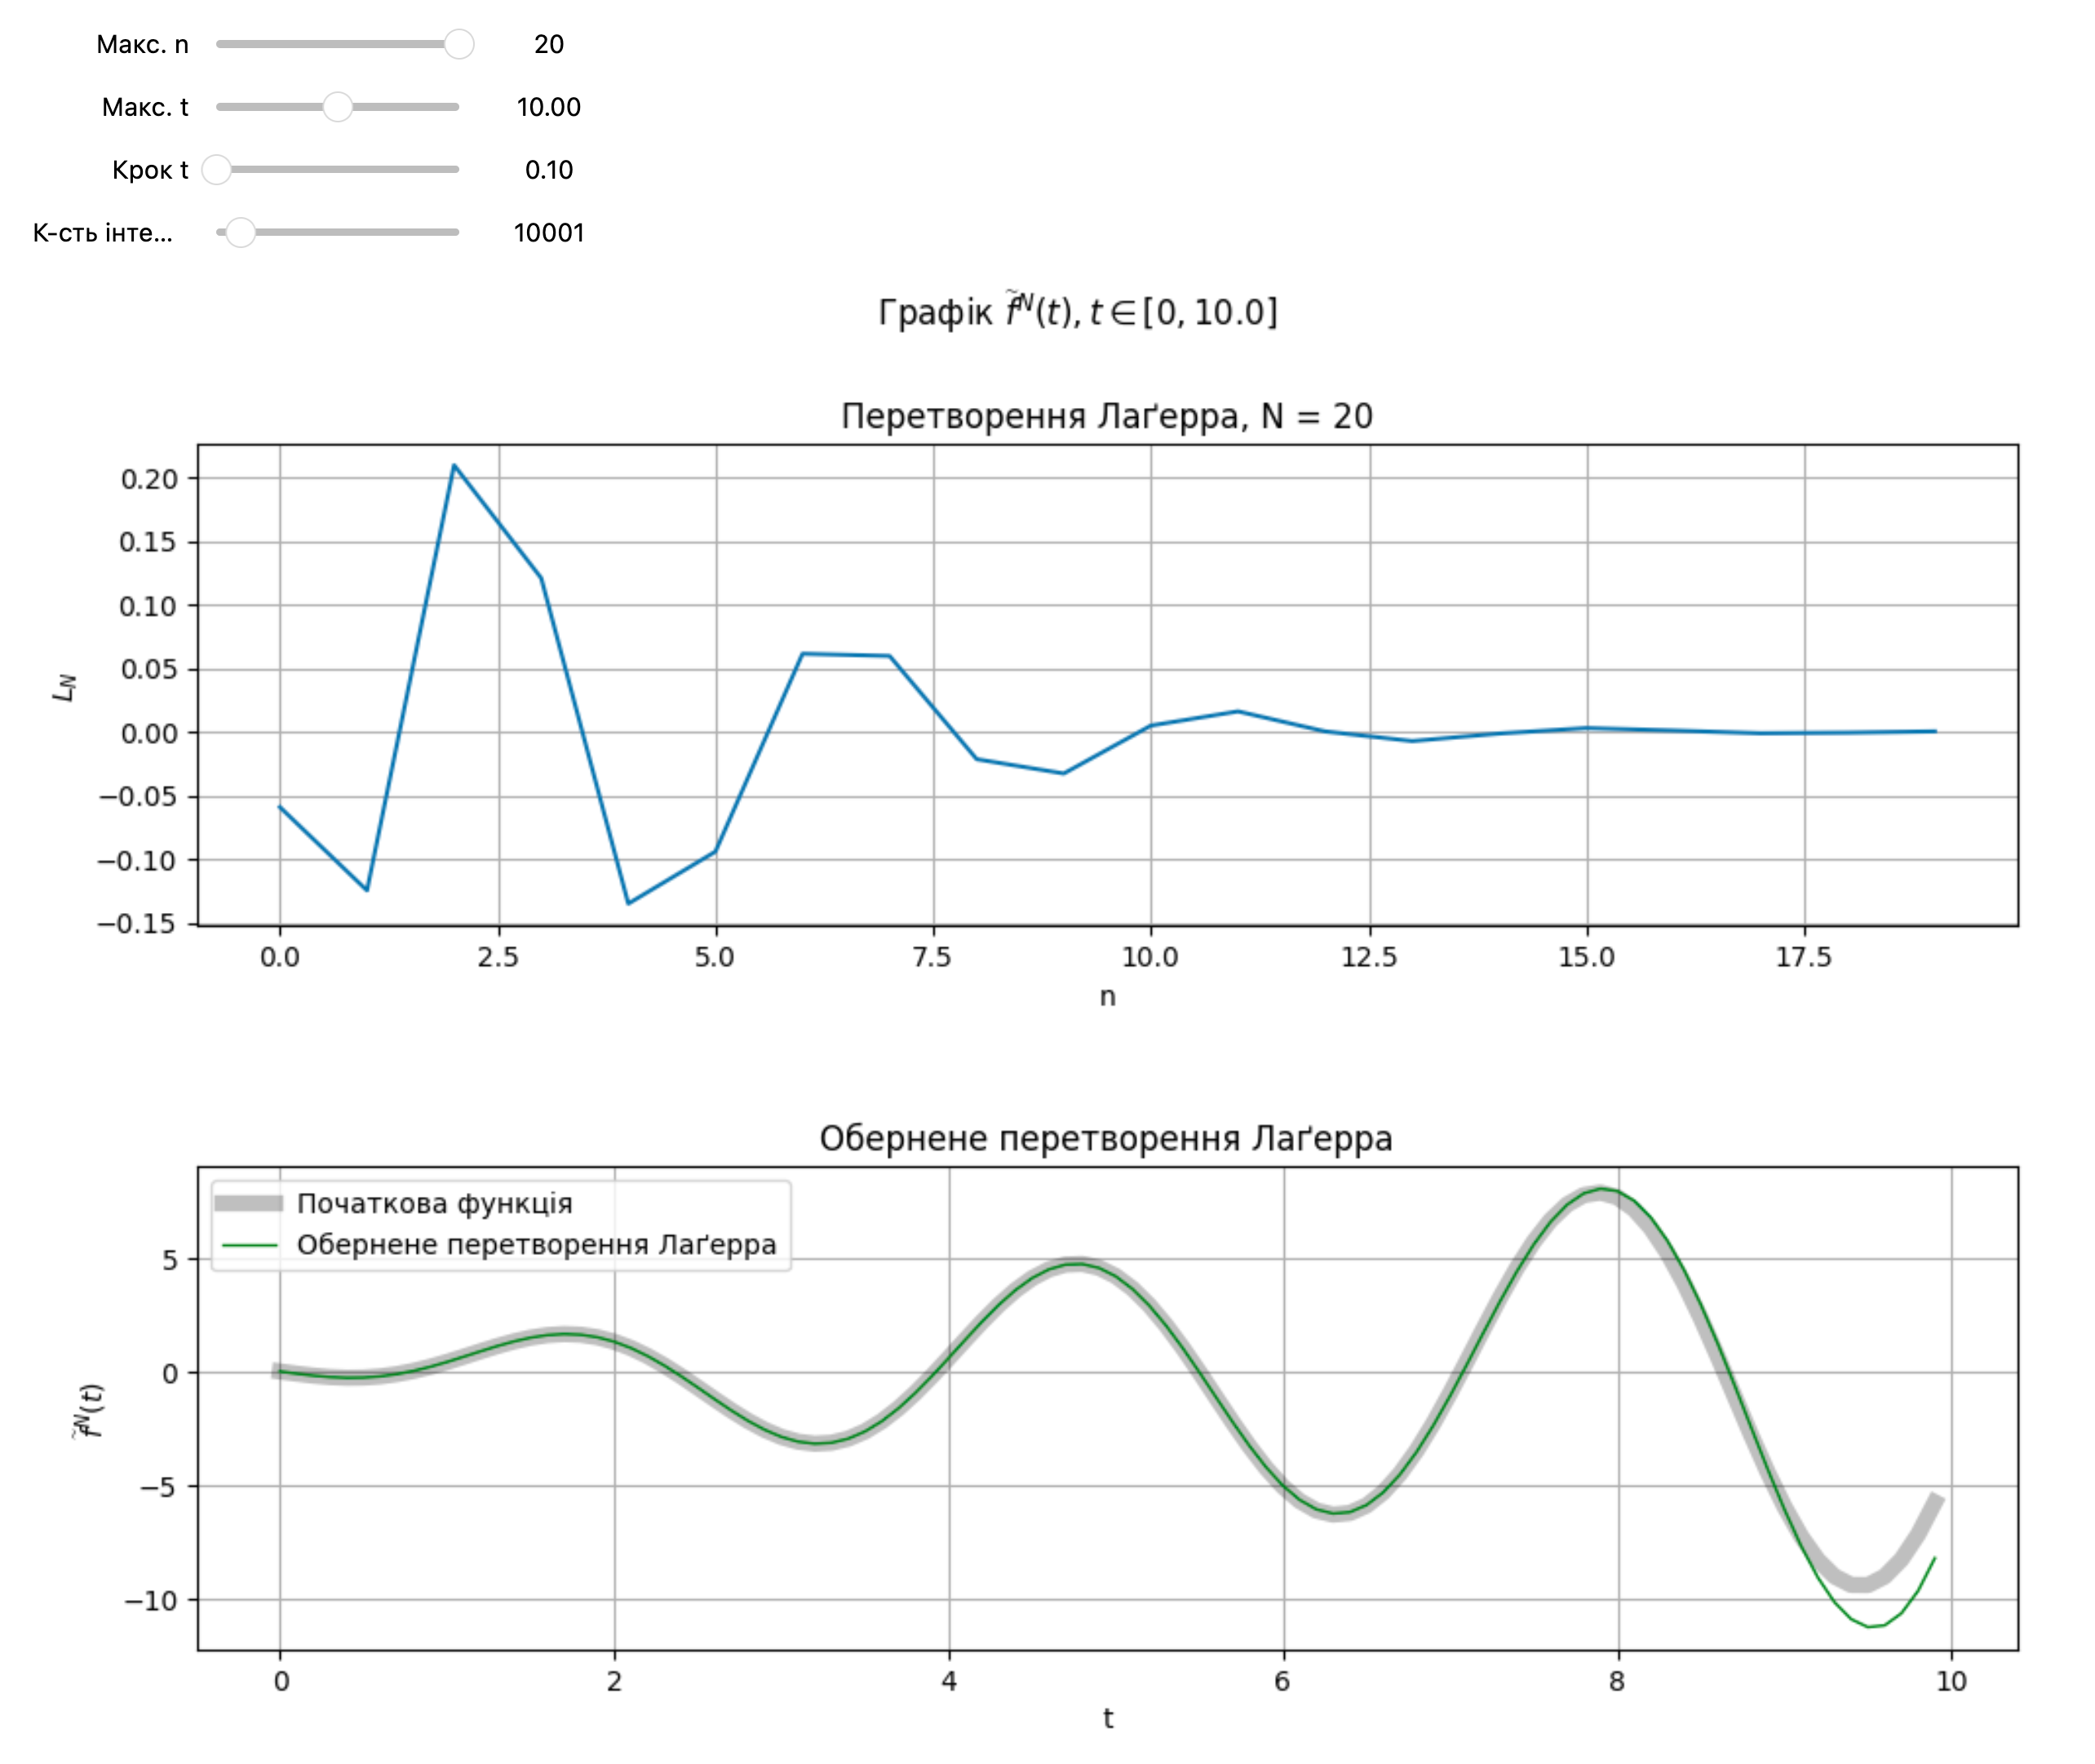
\includegraphics{screenshots/classes_10.png}
\caption{Widget screenshot}
\end{figure}

    \subsection*{Висновок}\label{ux432ux438ux441ux43dux43eux432ux43eux43a}

У лабораторній роботі було розглянуто використання многочленів Лаґерра у
контексті обчислення їхнього прямого та оберненого перетворення. Були
реалізовані функції для обчислення многочленів, їхньої табуляції,
проведення обчислювального експерименту для знаходження оптимального
значення аргументу t та обчислення перетворень.

В результаті роботи було показано, як можна використовувати многочлени
Лаґерра для перетворення функцій та як здійснювати обернене перетворення
для відновлення початкових функцій. Проведено аналіз та вивчення
залежностей між параметрами многочленів Лаґерра та їхніми властивостями.

Окремий акцент був зроблений на побудові графіків многочленів Лаґерра
для різних значень степенів. Це дозволило візуально спостерігати їхні
властивості та залежність від параметрів.

Також було проведено аналіз чотирьох функцій. Для них було побудовано
графіки перетворення Лаґерра та оберненого перетворення, що дозволило
візуально спостерігати схожість графіку оберненого перетворення та
початкової функції.

Отже, лабораторна робота надала можливість здобути практичні навички
використання многочленів Лаґерра, використовуючи об'єктно-орієнтований
підхід розробки програмного забезпечення.


    % Add a bibliography block to the postdoc
    
    
    
\end{document}
